% =====================================================================
%  Óbudai Egyetem – 64. Tudományos Diákköri Konferencia (2026. ősz)
%  TDK dolgozat: MIMIR – ellenőrizhető, adatvédelmet biztosító
%  vizsgakérdés-generálás lokális nyelvi modellekkel
%
%  Fordítás:  latexmk -pdf main.tex      (pdflatex + biber)
%  vagy:      pdflatex main && biber main && pdflatex main && pdflatex main
% =====================================================================
\documentclass[12pt,a4paper,oneside]{report}

% ---------------------------------------------------------------------
%  Kódolás, nyelv, betűkészlet
% ---------------------------------------------------------------------
\usepackage[utf8]{inputenc}
\usepackage[T1]{fontenc}
\def\magyarOptions{defaults=hu-min,postdescription=unchanged}
\usepackage[english,magyar]{babel}
\usepackage{mathptmx}                 % Times jellegű szövegtörzs
\usepackage[scaled=0.92]{helvet}
\usepackage{courier}
\usepackage{microtype}

% ---------------------------------------------------------------------
%  Oldalkép: A4, 2,5 cm margó, másfeles sorköz
% ---------------------------------------------------------------------
\usepackage[a4paper,top=2.5cm,bottom=2.5cm,left=2.5cm,right=2.5cm,headheight=15pt]{geometry}
\usepackage{setspace}
\onehalfspacing
\usepackage{fancyhdr}
\usepackage{titlesec}
\usepackage{enumitem}
\setlist{itemsep=2pt,topsep=4pt,parsep=0pt}

% ---------------------------------------------------------------------
%  Matematika, ábrák, táblázatok, algoritmusok
% ---------------------------------------------------------------------
\usepackage{amsmath,amssymb,amsthm}
\usepackage{bm}
\usepackage{graphicx}
\usepackage{booktabs}
\usepackage{array}
\usepackage{tabularx}
\usepackage{multirow}
\usepackage{makecell}
\usepackage{longtable}
\usepackage{float}
\usepackage[table]{xcolor}
\usepackage{caption}
\usepackage{subcaption}
\usepackage{siunitx}
\sisetup{output-decimal-marker={,},group-separator={\,},group-minimum-digits=4}
\usepackage{tikz}
\usetikzlibrary{arrows.meta,positioning,fit,backgrounds,shapes.geometric,calc,shadows}
\usepackage{pgfplots}
\pgfplotsset{compat=1.18}
\usepackage[ruled,vlined,linesnumbered,algochapter]{algorithm2e}
\usepackage{listings}
\usepackage{csquotes}

% ---------------------------------------------------------------------
%  Irodalomjegyzék (biblatex + biber, numerikus, megjelenési sorrend)
% ---------------------------------------------------------------------
\usepackage[backend=biber,style=numeric-comp,sorting=none,maxbibnames=6,minbibnames=3,
            giveninits=true,url=false,doi=true,isbn=false,eprint=true]{biblatex}
\addbibresource{references.bib}
\DeclareFieldFormat{titlecase}{#1}

% ---------------------------------------------------------------------
%  Hiperhivatkozások (utolsóként)
% ---------------------------------------------------------------------
\usepackage[hidelinks,unicode,bookmarksnumbered]{hyperref}
\usepackage{xurl}
\hypersetup{pdftitle={MIMIR: ellenőrizhető, adatvédelmet biztosító vizsgakérdés-generálás lokális nyelvi modellekkel},
            pdfsubject={TDK dolgozat, Óbudai Egyetem, 2026},
            pdfkeywords={kérdésgenerálás, RAG, kis nyelvi modellek, verifikáció, LLM-bíró}}

% ---------------------------------------------------------------------
%  Címlap adatai – KITÖLTENDŐ
% ---------------------------------------------------------------------
\newcommand{\Kar}{[Kar neve, pl. Neumann János Informatikai Kar]}
\newcommand{\Intezet}{[Intézet neve]}
\newcommand{\SzerzoA}{[Szerző 1 neve]}
\newcommand{\SzerzoAszak}{[szak, évfolyam]}
\newcommand{\SzerzoB}{[Szerző 2 neve]}
\newcommand{\SzerzoBszak}{[szak, évfolyam]}
\newcommand{\Konzulens}{[Konzulens neve]}
\newcommand{\KonzulensBeosztas}{[beosztás, intézet]}
\newcommand{\Ev}{2026}

\newcommand{\DolgozatCim}{Ellenőrizhető, adatvédelmet biztosító vizsgakérdés-generálás fogyasztói GPU-n futó kis nyelvi modellekkel}
\newcommand{\DolgozatAlcim}{A \textsc{Mimir} tervezésvezérelt, forráshivatkozásos RAG-módszere és többkarú kísérleti kiértékelése}

% ---------------------------------------------------------------------
%  Saját makrók
% ---------------------------------------------------------------------
\newcommand{\Mimir}{\textsc{Mimir}}
\newcommand{\tbd}[1]{\textcolor{red}{#1}}                   % csak a fő vizsgálat adatai
\newcommand{\code}[1]{\texttt{\small #1}}
\newcommand{\arm}[1]{\textsf{#1}}
\newcommand{\R}{\mathbb{R}}
\newcommand{\E}{\mathbb{E}}
\newcommand{\1}{\mathbb{1}}
\newcommand{\Doc}{\mathcal{D}}
\newcommand{\Chunks}{\mathcal{C}}
\newcommand{\Exam}{\mathcal{X}}
\newcommand{\argmax}{\operatorname*{arg\,max}}
\newcommand{\argmin}{\operatorname*{arg\,min}}
\DeclareMathOperator{\simop}{sim}

\theoremstyle{definition}
\newtheorem{definicio}{Definíció}[chapter]
\newtheorem{hipotezis}{Hipotézis}
\newtheorem{allitas}{Állítás}[chapter]
\theoremstyle{remark}
\newtheorem*{megjegyzes}{Megjegyzés}

% algorithm2e magyarítás
\SetAlgorithmName{Algoritmus}{algoritmus}{Algoritmusok jegyzéke}
\SetKwInput{KwIn}{Bemenet}
\SetKwInput{KwOut}{Kimenet}
\SetKwInput{KwParam}{Paraméterek}
\SetKw{KwRet}{visszatér}
\SetKwFor{ForEach}{minden}{elemre}{vége}
\SetKwFor{For}{ciklus}{:}{vége}
\SetKwFor{While}{amíg}{:}{vége}
\SetKwIF{If}{ElseIf}{Else}{ha}{akkor}{különben ha}{különben}{vége}
\SetAlFnt{\small}
\SetAlCapFnt{\small\bfseries}
\SetAlCapNameFnt{\small}

% listings – prompt- és konfigurációrészletek
\lstset{basicstyle=\ttfamily\scriptsize,breaklines=true,columns=fullflexible,frame=single,
        framerule=0.3pt,rulecolor=\color{gray!60},backgroundcolor=\color{gray!4},
        literate={á}{{\'a}}1 {é}{{\'e}}1 {í}{{\'i}}1 {ó}{{\'o}}1 {ö}{{\"o}}1 {ő}{{\H{o}}}1
                 {ú}{{\'u}}1 {ü}{{\"u}}1 {ű}{{\H{u}}}1 {Á}{{\'A}}1 {É}{{\'E}}1 {Í}{{\'I}}1
                 {Ó}{{\'O}}1 {Ö}{{\"O}}1 {Ő}{{\H{O}}}1 {Ú}{{\'U}}1 {Ü}{{\"U}}1 {Ű}{{\H{U}}}1
                 {–}{{--}}1 {„}{{,,}}1 {”}{{''}}1 {…}{{\ldots}}1}

% Fejezetcímek
\makeatletter
\newcommand\MimirChapterHeads{%
  \def\@makechapterhead##1{{\vspace*{-12pt}\normalfont\Large\bfseries
    \ifnum\c@secnumdepth>\m@ne\thechapter.\hspace{0.6em}\fi ##1\par\nobreak\vspace{16pt}}}%
  \def\@makeschapterhead##1{{\vspace*{-12pt}\normalfont\Large\bfseries ##1\par\nobreak\vspace{16pt}}}}
\addto\extrasmagyar{\MimirChapterHeads}
\AtBeginDocument{\MimirChapterHeads}
\makeatother
\titleformat{\section}{\normalfont\large\bfseries}{\thesection.}{0.5em}{}
\titleformat{\subsection}{\normalfont\normalsize\bfseries}{\thesubsection.}{0.5em}{}
\titleformat{\paragraph}[runin]{\normalfont\normalsize\bfseries}{\theparagraph}{0pt}{}
\titlespacing*{\paragraph}{0pt}{1.2ex plus .5ex minus .2ex}{0.6em}

% Élőfej / élőláb
\pagestyle{fancy}
\fancyhf{}
\fancyhead[L]{\small\itshape\Mimir{} -- ellenőrizhető vizsgakérdés-generálás}
\fancyhead[R]{\small\itshape\nouppercase{\leftmark}}
\fancyfoot[C]{\thepage}
\renewcommand{\headrulewidth}{0.4pt}
\fancypagestyle{plain}{\fancyhf{}\fancyfoot[C]{\thepage}\renewcommand{\headrulewidth}{0pt}}

\captionsetup{font=small,labelfont=bf,labelsep=period}
\setlength{\textfloatsep}{10pt plus 2pt minus 4pt}
\setlength{\floatsep}{8pt plus 2pt minus 2pt}
\setlength{\intextsep}{8pt plus 2pt minus 2pt}
\renewcommand{\topfraction}{0.85}
\renewcommand{\bottomfraction}{0.6}
\renewcommand{\textfraction}{0.12}
\renewcommand{\floatpagefraction}{0.75}
\makeatletter
\setlength{\@fptop}{0pt}
\setlength{\@fpsep}{16pt plus 4pt}
\setlength{\@fpbot}{0pt plus 1fil}
\makeatother
\renewcommand{\arraystretch}{1.12}

% =====================================================================
\begin{document}

% ------------------------------- CÍMLAP ------------------------------
\begin{titlepage}
\begin{center}
\begin{singlespace}
{\Large\bfseries ÓBUDAI EGYETEM\par}
\vspace{2mm}
{\large \Kar\par}
{\normalsize \Intezet\par}
\vspace{2mm}
\rule{\textwidth}{0.6pt}\par
\vspace{2.8cm}
{\LARGE\bfseries TUDOMÁNYOS DIÁKKÖRI DOLGOZAT\par}
\vspace{2.2cm}
{\Large\bfseries \DolgozatCim\par}
\vspace{6mm}
{\large\itshape \DolgozatAlcim\par}
\vfill
\begin{tabular}{@{}p{0.47\textwidth}p{0.47\textwidth}@{}}
\textbf{Szerzők:} & \textbf{Konzulens:}\\[1mm]
\SzerzoA & \Konzulens\\
\small\SzerzoAszak & \small\KonzulensBeosztas\\[3mm]
\SzerzoB & \\
\small\SzerzoBszak & \\
\end{tabular}
\vspace{2.4cm}

{\large Budapest, \Ev\par}
\vspace{2mm}
{\small 64. Tudományos Diákköri Konferencia -- \Ev.\ őszi félév\par}
\end{singlespace}
\end{center}
\end{titlepage}

% ------------------------- ELŐLAPOK (római számozás) -----------------
\pagenumbering{roman}
\setcounter{page}{2}
% ---------------------------------------------------------------------
%  Tartalmi összefoglaló (magyar) és Abstract (angol)
% ---------------------------------------------------------------------
\chapter*{Tartalmi összefoglaló}
\addcontentsline{toc}{chapter}{Tartalmi összefoglaló}
\thispagestyle{plain}

A feleletválasztós vizsgakérdések írása lassú és hibalehetőségekkel teli szakmai munka: a kérdésnek
egyértelműnek kell lennie, pontosan egy válaszlehetőségnek kell a tananyag szerint helyesnek lennie, a
disztraktoroknak pedig hihetőnek, de igazolhatóan hibásnak. A nagy nyelvi modellek (LLM) megjelenésével
a legelterjedtebb gyakorlat az lett, hogy az oktató feltölti a jegyzetét egy felhőben futó csevegő
asszisztensbe, és „tíz feleletválasztós kérdést” kér. Ez kényelmes, de négy lényeges hiányossága van:
(P1) semmi sem ellenőrzi, hogy a megjelölt helyes válasz valóban következik-e a dokumentumból;
(P2) a kérdések száma, típusa és nehézsége csak kérés, a hosszú bemenetet a modellek egyenetlenül
használják, így a kérdések néhány szakaszra tömörülnek; (P3) a tananyag egy harmadik félhez kerül;
(P4) a módszer nagy, távoli modellekre és hosszú kontextusra támaszkodik.

Dolgozatunkban bemutatjuk a \Mimir{} rendszert, amely a fenti egyetlen promptot explicit, ellenőrizhető
\emph{módszerrel} váltja fel, és egyetlen fogyasztói GPU-n futó, 7 milliárd paraméteres, 4 bitre kvantált
nyelvi modellel működik. A módszer lépései: szemantikus darabolás ablakozott mondatbeágyazással;
lefedettségvezérelt \emph{vizsgaterv} (blueprint), amely a fogalmakat, a kérdéstípusokat és a Bloom-szinteket
a legnagyobb maradék elvén osztja ki a slotokra; slotonkénti visszakeresés (sűrű vagy BM25\,+\,sűrű,
reciprok rangfúzióval); egyenként generált, forrásrészletekre hivatkozó kérdések; valamint a legolcsóbbtól
a legdrágábbig rendezett ellenőrző lánc (forma, meta-hivatkozás, hivatkozás, alátámasztottság és
disztraktorok, vak megoldhatóság, válaszszivárgás, duplikátum), amely hiba esetén visszacsatolással
újrapróbálkozik. Egy fogalomgráf-alapú változat (GraphRAG-lite) a tervezőt, a disztraktorjavaslatokat
és a kontextust gazdagítja. A rendszer mikroszolgáltatás-architektúrája zéró adatmegőrzést valósít meg:
a feltöltött tartalom csak a feladat idejére létezik, a naplóban csak kriptográfiai ujjlenyomatok maradnak.

Második hozzájárulásunk egy reprodukálható, nyílt kiértékelési \emph{módszertan}: tizenöt, egyszerre
egy tényezőt változtató kísérleti kar; 39 magyar és angol dokumentumból, 326 referenciakérdésből álló
adatkészlet; a generátoroktól eltérő modellcsaládba tartozó LLM-bíró; formálisan definiált mutatók
(formai megfelelés, alátámasztottság, vak megoldhatóság, disztraktor-validitás, lefedettség, szivárgás);
valamint dokumentumszintű statisztika (bootstrap konfidenciaintervallum, páros Wilcoxon-próba
Holm-korrekcióval, rangbiszeriális hatásméret, Krippendorff-$\alpha$).

Egy magyar dokumentumon végzett pilot (tíz kar, három ismétlés, 300 kérdés) szerint a helyi modell a
GPU-memóriából 5,4--5,9\,GB-ot foglal, tehát 8\,GB-os kártyán is fut. A pilot két, korábbi méréseket
érvénytelenítő mérési hibát és egy új hibamódot is feltárt: az ellenőrző visszacsatolási hurka a helyes
választ a kérdés szövegébe szivárogtatta, amit a bíró sem büntetett. A javított csővezetékkel végzett fő
vizsgálat (14 kar, kilenc magyar és angol dokumentum, karonként hat, 1\,670 kérdés) szerint a helyi 7B
modellel futó, tervezett és ellenőrzött csővezeték érte el a legmagasabb minőségi indexet (0,96; 95\,\%-os
CI: 0,93--0,98), szemben a naiv RAG (0,64), a teljes dokumentumot egy promptban kapó helyi modell (0,83) és
a teljes dokumentumot kapó nagy szervermodell (0,95) értékével. A tervezés 0,24-dal, az ellenőrzés -- a
pilottal ellentétben -- mind a hat dokumentumon 0,08-dal javított; a más modellcsaládba tartozó ellenőrző és
a fogalomgráf nem javított; a szivárgási szabályok a szivárgást 0--3\,\%-ra csökkentették; ugyanaz a
csővezeték a szervermodellel 0,99-et ért el. Az ellenőrző ítélete a bíróéval csak gyengén egyezik
(Cohen-$\kappa\le0{,}22$), a naiv RAG minőségét pedig a darabolás apró részletei is meghatározták. Hat
dokumentumon a különbségek a Holm-korrekció után nem szignifikánsak; a teljes, 39 dokumentumos futás és a
bíró oktatói validálása a következő lépés.

\medskip
\noindent\textbf{Kulcsszavak:} automatikus kérdésgenerálás, visszakereséssel kiegészített generálás (RAG),
kis nyelvi modellek, verifikáció, LLM-bíró, adatvédelem, oktatástechnológia, magyar nyelv

% ---------------------------------------------------------------------
\chapter*{Abstract}
\addcontentsline{toc}{chapter}{Abstract}
\thispagestyle{plain}

\begin{otherlanguage}{english}
The most common way to obtain an exam from teaching material today is to upload the document to a
hosted chat-based large language model (LLM) and ask for a test. This offers no evidence that the keyed
answers are supported by the document, no control over which parts of the material are covered, and it
discloses the material to a third party. We present \Mimir{}, an open system that generates
multiple-choice exams from a teacher's own documents with a 4-bit, 7-billion-parameter model running on a
single consumer GPU. \Mimir{} replaces the single prompt by an explicit method: semantic chunking with
windowed sentence encoding, a coverage-driven exam \emph{blueprint} that allocates concepts, question
types and Bloom levels to slots by the largest-remainder rule, per-slot dense or hybrid (BM25 + dense,
reciprocal rank fusion) retrieval, per-question generation with chunk citations, and a cheapest-first
verifier chain with feedback-driven retries, optionally enriched by a session-scoped concept graph. The
microservice architecture retains no uploaded content beyond the lifetime of a job.

We also contribute an evaluation methodology and open harness: fifteen single-factor experiment arms, a
39-document Hungarian--English dataset with 326 reference questions, a cross-family LLM judge, formally
defined measures and document-level statistics. A pilot on one Hungarian document (ten arms, three seeds,
300 questions) showed that the local model occupies 5.4--5.9\,GB of GPU memory, exposed two measurement
defects, and revealed an answer-leakage failure mode that inflates both automatic and LLM-judge scores. In
the main study with the corrected pipeline (14 arms, nine Hungarian and English documents, six per arm,
1,670 questions), the planned and verified pipeline on the local 7B model reached the highest quality index
(0.96, 95\,\% CI 0.93--0.98), against 0.64 for naive RAG, 0.83 for the whole document in one prompt to the
same model and 0.95 for the whole document to a large server model. Planning added 0.24; verification,
unlike in the pilot, added 0.08 on all six documents; a verifier from another model family and the concept
graph did not help; leakage rules cut leakage to 0--3\,\%; and the same pipeline on the server model reached
0.99. The verifier agrees only weakly with the judge (Cohen's $\kappa\le0.22$), and naive RAG proved fragile
to chunking details. With six documents no difference survives Holm correction; the full 39-document run and
the teachers' validation of the judge are the next step.

\medskip
\noindent\textbf{Keywords:} automatic question generation, retrieval-augmented generation, small language
models, verification, LLM-as-a-judge, privacy, educational technology, Hungarian
\end{otherlanguage}


\cleardoublepage
\phantomsection
\addcontentsline{toc}{chapter}{Tartalomjegyzék}
\begin{singlespace}
\tableofcontents
\end{singlespace}

% ---------------------------------------------------------------------
%  Rövidítések és jelölések
% ---------------------------------------------------------------------
\chapter*{Rövidítések és jelölések}
\addcontentsline{toc}{chapter}{Rövidítések és jelölések}
\thispagestyle{plain}

\begin{singlespace}
\subsection*{Rövidítések}
\begin{longtable}{@{}p{3.4cm}p{11.4cm}@{}}
AQG & \emph{Automatic Question Generation}, automatikus kérdésgenerálás\\
BM25 & \emph{Best Matching 25}, valószínűségi relevanciakeretre épülő lexikális rangsoroló függvény\\
CI & \emph{Confidence Interval}, konfidenciaintervallum\\
E5 & \emph{EmbEddings from bidirEctional Encoder rEpresentations}, kontrasztív szövegbeágyazó modellcsalád\\
GGUF & a \texttt{llama.cpp} kvantált modellformátuma\\
GQA & \emph{Grouped-Query Attention}, csoportosított lekérdezésű figyelem\\
GPU & \emph{Graphics Processing Unit}, grafikus feldolgozóegység\\
GDPR & az EU 2016/679 általános adatvédelmi rendelete\\
KV & \emph{key--value} (kulcs--érték) gyorsítótár a transzformer dekódolásakor\\
LLM & \emph{Large Language Model}, nagy nyelvi modell\\
MCQ & \emph{Multiple-Choice Question}, feleletválasztós kérdés\\
MRR & \emph{Mean Reciprocal Rank}, átlagos reciprok rang\\
Q4\_K\_M & 4 bites, csoportos K-kvantálás közepes változata (\texttt{llama.cpp})\\
RAG & \emph{Retrieval-Augmented Generation}, visszakereséssel kiegészített generálás\\
RQ & \emph{Research Question}, kutatási kérdés\\
RRF & \emph{Reciprocal Rank Fusion}, reciprok rangfúzió\\
SLM & \emph{Small Language Model}, kis nyelvi modell (itt: $\le$\,8 milliárd paraméter)\\
VRAM & a GPU dedikált memóriája\\
\end{longtable}

\subsection*{Fontosabb jelölések}
\begin{longtable}{@{}p{3.4cm}p{11.4cm}@{}}
$\Doc$ & a forrásdokumentum (karaktersorozat)\\
$S=(s_1,\dots,s_m)$ & a dokumentum mondatai\\
$\Chunks=(c_1,\dots,c_K)$ & a dokumentum darabjai (\emph{chunk}), $K=|\Chunks|$\\
$\phi(\cdot)\in\R^{d}$ & egységnyi normájú szövegbeágyazás ($d=768$, multilingual-E5-base)\\
$\delta_i$ & a szomszédos mondatok koszinusz-távolsága, $\delta_i = 1-\langle \phi(s_i),\phi(s_{i+1})\rangle$\\
$\tau$ & a darabolási alapküszöb (percentilis vagy $\mu+k\sigma$)\\
$\sigma=(n,T,\lambda,\ell)$ & vizsgaspecifikáció: kérdésszám, típusok, nehézség, nyelv\\
$q=(t,O,o^\star,R)$ & kérdés: törzs, válaszlehetőségek, kulcs, hivatkozott darabok\\
$\Exam=(q_1,\dots,q_n)$ & a generált vizsga\\
$\mathcal{B}=\{(\kappa_j,T_j,b_j)\}$ & a vizsgaterv slotjai: fogalom, típus, Bloom-szint\\
$G(q),\,A(q),\,V(q)$ & alátámasztottság, vak megoldhatóság, disztraktor-validitás (bírói ítéletek)\\
$F(\Exam)$ & formai megfelelés indikátora\\
$\mathrm{Cov}(\Exam)$ & darablefedettség\\
$Q(\Exam)$ & minőségi index, a négy ráta átlaga\\
$L(q)$ & válaszszivárgás indikátora (kulcs a törzsben)\\
$\kappa$ & Cohen-féle egyezési együttható (a szövegkörnyezetből egyértelmű, hogy nem fogalom)\\
$\alpha$ & Krippendorff-féle megbízhatósági együttható\\
$r_{rb}$ & páros rangbiszeriális hatásméret\\
\end{longtable}
\end{singlespace}


% ----------------------------- FŐSZÖVEG ------------------------------
\cleardoublepage
\pagenumbering{arabic}
\setcounter{page}{1}

% =====================================================================
\chapter{Bevezetés}
\label{ch:bevezetes}
% =====================================================================

\section{Motiváció}

A felsőoktatásban és a középiskolában a feleletválasztós kérdés (\emph{multiple-choice question}, MCQ)
a tudásmérés egyik legszélesebb körben használt eszköze: gépi úton javítható, nagy létszámú kurzusokon is
skálázható, és jól illeszkedik a tanulásmenedzsment-rendszerek (pl.\ Moodle) kvízmoduljaihoz. Előállítása
azonban drága. A pszichometriai szakirodalom szerint egy jó kérdés törzse önmagában is érthető és
egyértelmű, pontosan egy válaszlehetősége helyes a tananyag szerint, a disztraktorok pedig azonos
témájúak, formailag hasonlóak és egy felkészületlen hallgató számára hihetők, ám igazolhatóan
hibásak~\cite{haladyna2002review,gierl2017distractors}. Egy tapasztalt oktató egy-egy ilyen kérdésen
perceket, egy teljes vizsgán órákat dolgozik, és a disztraktorok megírása a munka legnehezebb része.

A nagy nyelvi modellek (\emph{large language model}, LLM) megjelenése~\cite{brown2020gpt3} gyökeresen
átalakította ezt a munkafolyamatot. Az oktatástechnológiai irodalom egyszerre hangsúlyozza a lehetőségeket
és a kockázatokat~\cite{kasneci2023chatgpt}: a modellek képesek kérdéseket és disztraktorokat
fogalmazni~\cite{kurdi2020systematic,alhazmi2024distractor}, ugyanakkor hajlamosak folyékony, de a forrás
által nem alátámasztott állításokat generálni~\cite{ji2023hallucination}. A gyakorlatban a
legelterjedtebb használati mód a legegyszerűbb: az oktató feltölti az előadásjegyzetét egy felhőben futó
csevegő asszisztensbe, és „tíz feleletválasztós kérdést” kér. Ezt a munkafolyamatot a továbbiakban
\emph{status quo}-nak vagy \emph{közvetlen megközelítésnek} nevezzük.

\section{Problémafelvetés}

A közvetlen megközelítés kényelmes, de az iskolai alkalmazás szempontjából négy, egymástól független
gyengesége van. Ezek adják dolgozatunk kiindulópontját.

\begin{description}[leftmargin=1.1cm,labelwidth=0.9cm,style=sameline,format=\normalfont\bfseries]
\item[(P1)] \textbf{A helyesség nincs ellenőrizve.} Semmi sem garantálja, hogy a megjelölt kulcsot a
dokumentum alátámasztja, és hogy a disztraktorok valóban hamisak. Az LLM-ek hihető, de alá nem támasztott
állításokat állítanak elő~\cite{ji2023hallucination}; az önellenőrzés ezt csökkentheti, de nem
szünteti meg~\cite{madaan2023selfrefine,dhuliawala2024cove,huang2024selfcorrect}.
\item[(P2)] \textbf{A szerkezet és a lefedettség nincs kontrollálva.} A kért darabszám, típus és nehézség
csak kérés a promptban. A hosszú bemenetet a modellek egyenetlenül használják: a kontextus elejére és
végére jobban figyelnek, mint a közepére~\cite{liu2024lost}, a névleges kontextushossznál jóval rövidebb
az a hossz, amelyen még megbízhatóan dolgoznak~\cite{hsieh2024ruler}. Ennek következménye, hogy a kérdések
a dokumentum néhány szakaszára tömörülnek.
\item[(P3)] \textbf{Adatvédelem.} A tananyag személyes adatot (pl.\ esettanulmányban szereplő neveket,
hallgatói munkákat) is tartalmazhat; a felhőszolgáltatás az adatkezelés címzettjévé
válik~\cite{gdpr2016}, az intézmény pedig elveszíti a kontrollt a tartalom sorsa felett.
\item[(P4)] \textbf{Függés a nagy, távoli modellektől.} A teljes dokumentum egyetlen promptban hosszú
kontextust és nagy modellt igényel. Az iskola által saját hardveren futtatható kis modellek (néhány
milliárd paraméter, 8\,GB videomemória) kontextusa és memóriája korlátos.
\end{description}

Fontos látni, hogy a négy probléma nem oldható meg egyszerűen „jobb prompttal”. A P1 és a P2 a
\emph{módszer} hiányából fakad: ha a vizsga szerkezete, a kérdések forrása és az ellenőrzés nem explicit
lépések, akkor nem is mérhetők és nem is kényszeríthetők ki. A P3 és a P4 pedig egymást erősítik: a
helyi futtatás megoldaná az adatvédelmi problémát, de a helyben futtatható kis modellek éppen a hosszú
kontextusú, egylépéses feladatban a leggyengébbek. Kutatásunk alapgondolata ezért az, hogy a
feladatot rövid, jól specifikált, egyenként ellenőrizhető lépésekre bontva egy kis, helyben futó modell
is képes lehet megbízható vizsgát előállítani, és ez a felbontás egyben a P1 és P2 problémát is kezeli.

\section{Kutatási kérdések és hipotézisek}

A fenti problémák alapján három kutatási kérdést fogalmaztunk meg.

\begin{description}[leftmargin=1.3cm,labelwidth=1.1cm,style=sameline,format=\normalfont\bfseries]
\item[RQ1] A strukturált generálás -- tervezés, kérdésenkénti forráshoz kötés és ellenőrzés -- érvényesebb
és jobban lefedő vizsgát eredményez-e, mint ha a modellnek a dokumentumot (vagy annak visszakeresett
részleteit) egyetlen promptban adjuk át?
\item[RQ2] Mennyivel járul hozzá a minőséghez az egyes komponens (tervező, ellenőrző, fogalomgráf,
hibrid visszakeresés, darabolási stratégia), és mennyibe kerül futási időben, modellhívásban és
tokenben?
\item[RQ3] Mennyire közelíti meg egy 8\,GB-os fogyasztói GPU-n futó, 4 bitre kvantált 7B modell egy
nagy, szerveren futó modell teljesítményét?
\end{description}

A kutatási kérdésekhez a következő hipotéziseket rendeljük. Értékelésüket a pilot és a fő vizsgálat
alapján \az{\ref{sec:hipotezis-ertekeles}}.~szakasz adja.

\begin{hipotezis}[Tervezés]\label{h:terv}
Azonos generátormodell mellett a vizsgaterv (\arm{E1}) a naiv RAG alapvonalhoz (\arm{E0}) képest
növeli a kérdések alátámasztottságát és a vizsga darablefedettségét, a formai megfelelés romlása nélkül.
\end{hipotezis}

\begin{hipotezis}[Ellenőrzés]\label{h:verif}
Az ellenőrző lánc (\arm{E2}) a tervezéshez (\arm{E1}) képest tovább növeli az alátámasztottságot és a
vak megoldhatóságot; az ellenőrző ítélete pozitívan egyezik a független bíró ítéletével ($\kappa>0$).
\end{hipotezis}

\begin{hipotezis}[Lefedettség]\label{h:lefed}
A teljes dokumentumot egyetlen promptban kapó alapvonal (\arm{B-doc}) lefedettsége -- modellmérettől
függetlenül -- alacsonyabb, mint a tervezett változatoké.
\end{hipotezis}

\begin{hipotezis}[Helyi vs.\ szerver]\label{h:helyi}
A helyi 7B modell a tervezett és ellenőrzött csővezetékben a szervermodell naiv változatának
minőségi indexét megközelíti (különbség $<0{,}1$), miközben a GPU-memóriaigénye 8\,GB alatt marad.
\end{hipotezis}

\begin{hipotezis}[Mérés]\label{h:meres}
A generátoroktól eltérő modellcsaládba tartozó LLM-bíró ítéletei az oktatói értékelésekkel legalább
elfogadható megbízhatósággal egyeznek (Krippendorff-$\alpha\ge 0{,}667$).
\end{hipotezis}

\section{Hozzájárulások}

Dolgozatunk négy, egymásra épülő hozzájárulást tartalmaz.

\begin{enumerate}[label=(\arabic*)]
\item \textbf{A \Mimir{} generálási módszer} (\ref{ch:modszer}.~fejezet): ablakozott mondatbeágyazáson
alapuló szemantikus darabolás, lefedettségvezérelt vizsgaterv a legnagyobb maradék elvén kiosztott
Bloom-szintekkel, slotonkénti sűrű vagy hibrid visszakeresés, forrásrészletekre hivatkozó egyenkénti
kérdésgenerálás, legolcsóbbtól a legdrágábbig rendezett ellenőrző lánc visszacsatolással és
tartalékfogalmakkal, valamint egy munkamenet-hatókörű fogalomgráf (GraphRAG-lite). A módszert formálisan
is megfogalmazzuk (\ref{ch:formalizmus}.~fejezet), és algoritmikusan leírjuk.
\item \textbf{Adatvédelmet biztosító helyi architektúra} (\ref{ch:architektura}.~fejezet): lazán
csatolt mikroszolgáltatások, PostgreSQL-alapú zárolásmentes feladatsor, zéró adatmegőrzés és
ujjlenyomat-alapú audit, valamint a GPU-memóriaigény analitikus modellje, amelyet mérésekkel
validálunk.
\item \textbf{Kiértékelési módszertan és nyílt keretrendszer} (\ref{ch:kiertekeles}.~fejezet): tizenöt
egytényezős kísérleti kar, kétnyelvű adatkészlet referenciakérdésekkel, formálisan definiált mutatók,
modellcsaládon kívüli LLM-bíró, oktatói értékelési protokoll és dokumentumszintű statisztika.
\item \textbf{Empirikus eredmények} (\ref{ch:eredmenyek}.~fejezet): egy pilot vizsgálat, amely két
korábbi méréseket érvénytelenítő mérési hibát, a válaszszivárgást mint új hibamódot és a futásról futásra
jelentkező zajt tárta fel, valamint egy 14 karos, kilenc dokumentumos fő vizsgálat, amely szerint a helyi
7B modellel futó tervezett és ellenőrzött csővezeték a közös dokumentumokon a naiv RAG-ot ($0{,}64$) és a
teljes dokumentumos promptot ($0{,}83$) is felülmúlta ($0{,}96$), és elérte a teljes dokumentumot kapó
szervermodellt ($0{,}95$).
\end{enumerate}

\section{A dolgozat felépítése}

\Az{\ref{ch:szakirodalom}}.~fejezet áttekinti az automatikus kérdésgenerálás, a visszakereséssel
kiegészített generálás, az ellenőrzés és a nyelvimodell-alapú kiértékelés szakirodalmát, és
azonosítja a kutatási rést. \Az{\ref{ch:formalizmus}}.~fejezet a feladatot formálisan definiálja,
bevezeti a minőségi predikátumokat és a célfüggvényt. \Az{\ref{ch:architektura}}.~fejezet a rendszer
architektúráját, adatvédelmi mechanizmusait és erőforrás-modelljét mutatja be. \Az{\ref{ch:modszer}}.~fejezet a generálási módszer algoritmusait és azok költségelemzését tárgyalja.
\Az{\ref{ch:kiertekeles}}.~fejezet a kiértékelési módszertant, \az{\ref{ch:eredmenyek}}.~fejezet a pilot és a fő
vizsgálat eredményeit ismerteti. \Az{\ref{ch:diszkusszio}}.~fejezet az eredmények értelmezését és az érvényességet
veszélyeztető tényezőket, \az{\ref{ch:osszefoglalas}}.~fejezet az összefoglalást és a további munkát
tartalmazza. A függelék a promptokat, a konfigurációkat és a reprodukálás lépéseit közli.

% =====================================================================
\chapter{Szakirodalmi áttekintés}
\label{ch:szakirodalom}
% =====================================================================

Ebben a fejezetben azokat a kutatási irányokat tekintjük át, amelyekre a \Mimir{} módszere és
kiértékelése épül: az automatikus kérdés- és disztraktorgenerálást, a visszakereséssel kiegészített
generálást, a hosszú kontextus problémáit, az ellenőrzést és önjavítást, a kis és kvantált modelleket,
valamint a nyelvi modellekkel végzett kiértékelést. A fejezet végén összevetjük a meglévő
megközelítéseket, és megfogalmazzuk a kutatási rést.

\section{Automatikus kérdésgenerálás}

Az automatikus kérdésgenerálás (\emph{automatic question generation}, AQG) több évtizedes múltra
tekint vissza. Kurdi és munkatársai szisztematikus irodalmi áttekintése~\cite{kurdi2020systematic}
93 oktatási célú AQG-rendszert elemzett, és három generációt különített el. Az \emph{első} generáció
szabály- és sablonalapú: szintaktikai elemzéssel azonosítja a kérdezhető mondatrészeket, és
transzformációs szabályokkal kérdő mondattá alakítja őket. Mitkov és Ha rendszere~\cite{mitkov2003computer}
például főnévi csoportokat választ ki kulcsként, és a kulcshoz szemantikusan közeli fogalmakat
(WordNet-szomszédokat) javasol disztraktornak. Heilman és Smith~\cite{heilman2010good} a túlgenerálás és
rangsorolás elvét vezette be: a szabályok sok jelöltet állítanak elő, amelyeket egy statisztikai modell
rangsorol. A \emph{második} generáció neurális szekvencia--szekvencia modelleket használ; Du és
munkatársai~\cite{du2017learning} figyelemmechanizmusos kódoló--dekódoló hálózattal olvasásértési
kérdéseket generáltak. A \emph{harmadik} generációt az előtanított transzformerek~\cite{vaswani2017attention,devlin2019bert}
és a nagy nyelvi modellek~\cite{brown2020gpt3} jelentik, amelyek utasításkövetéssel, finomhangolás nélkül
is képesek kérdés--válasz párokat írni.

Az áttekintések visszatérő megállapítása, hogy a kiértékelés a terület gyenge pontja. Mulla és
Gharpure~\cite{mulla2023aqg} szerint a rendszerek jelentős részét referencia-átfedésen alapuló
metrikákkal (BLEU~\cite{papineni2002bleu}, ROUGE~\cite{lin2004rouge}) mérik, amelyek egy referenciakérdéshez
való lexikális hasonlóságot jutalmaznak. Egy vizsgakérdés azonban akkor is kiváló lehet, ha egyetlen
szava sem egyezik a referenciával, és akkor is használhatatlan, ha a kulcsa hibás. A humán értékelések jellemzően kis mintán, nem vakon
történnek, és ritkán ellenőrzik a kulcs helyességét~\cite{kurdi2020systematic}. Munkánkban ezért a referenciakérdéseket nem célként, hanem csak a visszakeresés és a
tematikus hasonlóság mérésére használjuk, a helyességet pedig explicit, forrásalapú predikátumokkal mérjük.

\section{Disztraktorgenerálás és tesztelméleti követelmények}

A feleletválasztós kérdés minőségét döntően a disztraktorok határozzák meg. Haladyna, Downing és
Rodriguez~\cite{haladyna2002review} 31 kérdésírási irányelvet összegző munkája szerint a disztraktoroknak
hihetőnek, egymást kölcsönösen kizárónak, a kulccsal azonos hosszúságúnak és nyelvtani formájúnak kell
lenniük, és kerülni kell a „mindegyik fenti” típusú opciókat. Gierl és munkatársai~\cite{gierl2017distractors}
áttekintése a disztraktorok kidolgozásának, elemzésének és felhasználásának gyakorlatát foglalja össze,
és rámutat, hogy a nem funkcionáló (senki által nem választott) disztraktor gyakorlatilag csökkenti az
opciók számát, így növeli a találgatás esélyét.

Alhazmi és munkatársai~\cite{alhazmi2024distractor} a disztraktorgenerálás módszereit három csoportba
sorolják: tudásbázis- és ontológiaalapú (hasonló fogalmak lexikai adatbázisból), korpuszalapú (disztribúciós
hasonlóság) és generatív (neurális vagy LLM-alapú) módszerekre. Megállapításuk szerint a generatív
módszerek a legfolyékonyabb disztraktorokat adják, ám gyakran előfordul, hogy egy disztraktor valójában
szintén helyes, vagy nyilvánvalóan abszurd. A \Mimir{} ezt két ponton kezeli: a fogalomgráf-alapú változat
a dokumentumból kinyert \emph{testvérfogalmakat} (azonos szülőfogalom alá tartozó fogalmakat) ajánlja
disztraktor-ötletként, az ellenőrző pedig minden disztraktorra külön ítéletet kér arról, hogy a forrás
szerint hamis-e.

\section{A kognitív szint: Bloom taxonómiája}

A kérdések nehézségének szabályozására a legelterjedtebb keret Bloom taxonómiája~\cite{bloom1956taxonomy}
és annak Anderson és Krathwohl által átdolgozott változata~\cite{anderson2001bloom}. A revideált taxonómia
kognitív dimenziója hat, egymásra épülő szintet különít el: emlékezés, megértés, alkalmazás, elemzés,
értékelés és alkotás. A feleletválasztós formátum az első öt szint mérésére alkalmas; az alkotás
jellemzően nyitott feladatot igényel. A \Mimir{} a kért nehézséghez egy Bloom-szinteloszlást rendel
(\ref{sec:blueprint}.~szakasz), és ezt az eloszlást a legnagyobb maradék elvén diszkretizálja a
vizsga slotjaira, így a nehézség a promptban tett kérés helyett a terv szerkezeti tulajdonsága lesz.

\section{Visszakereséssel kiegészített generálás}

A visszakereséssel kiegészített generálás (RAG) Lewis és munkatársai~\cite{lewis2020rag} munkájában
jelent meg: egy sűrű visszakereső (DPR~\cite{karpukhin2020dpr}) a kérdéshez releváns szövegrészleteket
keres egy külső korpuszból, és a generátor ezekre támaszkodva válaszol. Azóta a RAG a nyelvi modellek
tényszerűségének növelésére szolgáló legelterjedtebb technikává vált; Gao és munkatársai
áttekintése~\cite{gao2023ragsurvey} a „naiv”, a „fejlett” és a „moduláris” RAG paradigmáit különíti el.
A naiv RAG egyetlen visszakeresést és egyetlen generálást végez; a fejlett RAG a visszakeresés előtt
és után optimalizál (lekérdezés-átírás, újrarangsorolás); a moduláris RAG pedig tetszőleges sorrendben
kombinálja a visszakeresési, generálási és ellenőrzési modulokat. A \Mimir{} tervezett csővezetéke
ebben a terminológiában moduláris RAG: a visszakeresés a terv minden slotjára külön fut, és az ellenőrzés
eredménye visszacsatol a visszakeresésre.

\paragraph{Sűrű és lexikális visszakeresés.} A sűrű visszakeresés a szövegeket egy közös vektortérbe
képezi. A mondatbeágyazások Sentence-BERT óta~\cite{reimers2019sbert} sziámi hálózatokkal, kontrasztív
tanítással készülnek; az E5 modellcsalád~\cite{wang2022e5} gyengén felügyelt kontrasztív előtanítással
készült, többnyelvű változata~\cite{wang2024me5} a magyart is támogatja. A lexikális visszakeresés
klasszikus módszere a BM25~\cite{robertson2009bm25}, amely a kifejezésgyakoriságot telítő függvénnyel és
dokumentumhossz-normalizálással súlyozza. A két módszer hibái eltérnek: a sűrű visszakeresés a
szinonimákat és parafrázisokat kezeli jól, a lexikális a ritka szakkifejezéseket és tulajdonneveket. Az
eredmények egyesítésére a reciprok rangfúzió (RRF)~\cite{cormack2009rrf} egyszerű és robusztus
módszer, amely csak a rangokat használja, így nem igényli a heterogén pontszámok kalibrálását.

\paragraph{Darabolás.} A visszakeresés egysége a darab (\emph{chunk}). A rögzített méretű ablakok
egyszerűek, de mondatok és gondolatmenetek közepén vágnak. A szemantikus darabolás a szomszédos mondatok
beágyazásainak távolságát figyeli, és ott vág, ahol a téma megváltozik. Qu, Tu és Bao~\cite{qu2024chunking}
szisztematikusan vizsgálták, megéri-e a szemantikus darabolás számítási többletköltsége, és azt találták,
hogy előnye adatkészletfüggő, és gyakran kisebb, mint várnánk. Ez indokolja, hogy a darabolási stratégiát
mi is külön kísérleti karokkal (\arm{E5a--c}) vizsgáljuk, ahelyett hogy eleve jobbnak tekintenénk.

\paragraph{Gráfalapú RAG.} Edge és munkatársai GraphRAG módszere~\cite{edge2024graphrag} a korpuszból
nyelvi modellel entitás- és relációgráfot épít, a gráfot közösségekre bontja, és a közösségek
összefoglalóival válaszol a korpusz egészére vonatkozó („globális”) kérdésekre. A módszer drága: a teljes
korpuszt többször fel kell dolgozni. A \Mimir{} ennek egy könnyített, munkamenet-hatókörű változatát
használja: a fogalomgráf egyetlen dokumentumra, kötegenként egy hívással készül, és csak a vizsga
élettartamáig létezik.

\section{Hosszú kontextus: az egylépéses alternatíva korlátai}

A RAG alternatívája az, hogy a teljes dokumentumot egyetlen promptban adjuk át a modellnek -- ez
felel meg az oktatók napi gyakorlatának. Liu és munkatársai~\cite{liu2024lost} kimutatták, hogy a
modellek teljesítménye U alakú függvénye a releváns információ pozíciójának: a kontextus elején és végén
elhelyezett információt jobban használják, mint a közepén lévőt („lost in the middle”). Hsieh és
munkatársai RULER benchmarkja~\cite{hsieh2024ruler} szerint a legtöbb modell „tényleges” kontextushossza
jóval rövidebb a névlegesnél. Vizsgagenerálásra vetítve ez azt jelenti, hogy a teljes dokumentumot kapó
modell kérdései várhatóan a dokumentum elejére és végére tömörülnek, ami a lefedettség mérésével
közvetlenül tesztelhető (\ref{h:lefed}.~hipotézis).

\section{Hallucináció, ellenőrzés és önjavítás}

Ji és munkatársai~\cite{ji2023hallucination} a hallucinációt úgy definiálják, mint a forrással
ellentmondó (\emph{intrinzikus}) vagy abból nem igazolható (\emph{extrinzikus}) generált tartalmat. A
kérdésgenerálásban mindkettő előfordul: a kulcs ellentmondhat a forrásnak, vagy olyan tényen alapulhat,
amely a forrásban nem szerepel.

A hallucináció csökkentésére az irodalom két nagy stratégiát javasol. Az \emph{önjavító} módszerek
(Self-Refine~\cite{madaan2023selfrefine}) a modell saját visszajelzésére építve iteratívan javítják a
kimenetet; a Chain-of-Verification~\cite{dhuliawala2024cove} ellenőrző kérdéseket generál, ezekre
egymástól függetlenül válaszol, majd a válaszok alapján módosítja az eredeti kimenetet. A SelfCheckGPT~\cite{manakul2023selfcheck}
mintavételezett válaszok konzisztenciájából becsüli a hallucinációt, a FActScore~\cite{min2023factscore}
pedig atomi tényekre bontja a szöveget, és ezeket egyenként ellenőrzi egy tudásforrással szemben.
Huang és munkatársai~\cite{huang2024selfcorrect} ugyanakkor kimutatták, hogy külső visszajelzés nélkül a
modellek önjavítása érvelési feladatokban nem javít, sőt ronthat is. Snell és
munkatársai~\cite{snell2025scaling} azt mutatták meg, hogy a következtetési időben elköltött számítás
(több minta, ellenőrzés) bizonyos feladatokban helyettesítheti a modellméretet -- ez adja az elméleti
alapját annak, hogy egy kis modell ellenőrző lánccal megközelítheti egy nagy modell minőségét.

A \Mimir{} ellenőrző lánca e két irány metszetében helyezkedik el: külső, determinisztikus szabályokat
(forma, meta-hivatkozás, hivatkozás, szivárgás, duplikátum) kombinál a forrással szembeni, nyelvi
modellel végzett ítéletekkel (alátámasztottság, disztraktorok, vak megoldás). Pilot eredményeink
(\ref{sec:verifier-eredmeny}.~szakasz) Huang és munkatársai megállapításával összhangban azt mutatják,
hogy a generátorral azonos kis modellel végzett ítélet nem hordoz érdemi információt.

\section{Kis nyelvi modellek és kvantálás}

A helyi futtatás kulcskérdése a memória. Egy $P$ paraméteres modell súlyai 16 bites lebegőpontos
ábrázolásban $2P$ bájtot foglalnak, ami 7 milliárd paraméternél 14\,GB -- ez nem fér el egy fogyasztói
kártyán. A kvantálás a súlyokat alacsonyabb bitszámon tárolja: az LLM.int8()~\cite{dettmers2022int8}
8 bites, a GPTQ~\cite{frantar2023gptq} 3--4 bites utólagos kvantálást vezetett be. A \texttt{llama.cpp}
projekt~\cite{gerganov2023llamacpp} GGUF formátuma és csoportos K-kvantálása (pl.\ Q4\_K\_M) a helyi
futtatás de facto szabványa lett; erre épül az általunk használt Ollama futtatókörnyezet~\cite{ollama2024}.
Átfogó kiértékelések szerint a 4 bites súlykvantálás általános benchmarkokon csak kis
pontosságvesztést okoz~\cite{li2024evalquant,kurtic2025bf16,kurt2026quant}. A memóriaigény másik összetevője a kulcs--érték (KV) gyorsítótár, amely a kontextushosszal
lineárisan nő; a csoportosított lekérdezésű figyelem (GQA)~\cite{ainslie2023gqa} a KV-fejek számának
csökkentésével ezt jelentősen mérsékli, a PagedAttention~\cite{kwon2023vllm} pedig a töredezettséget
szünteti meg; a helyi futtatás energiaigényét fogyasztói hardveren Zähl és Hennig mérte~\cite{zahl2026energy}.

Az oktatási kérdésgenerálásban Fawzi és munkatársai~\cite{fawzi2023small,fawzi2024towards} kimutatták,
hogy kis modellek további előtanítással és finomhangolással a nagy modellekhez mérhető kérdéseket
állíthatnak elő, Jaldi és munkatársai~\cite{jaldi2026small} pedig kis, privát modelleket hasonlítottak
össze nagy modellekkel Bloom-szintekhez igazított értékelés tervezésében. A mi megközelítésünk ezektől
abban tér el, hogy finomhangolás nélküli, általános célú modellt használunk, és a minőséget a
\emph{módszer} szerkezetével (terv, forráshoz kötés, ellenőrzés) igyekszünk biztosítani.

\begin{table}[tbp]
\centering
\caption{A kérdésgenerálási megközelítések összevetése a P1--P4 problémák szempontjából
(\checkmark: megoldott, $\circ$: részben, --: nem kezelt).}
\label{tab:irodalom-osszevetes}
\small
\setlength{\tabcolsep}{4pt}
\resizebox{\textwidth}{!}{%
\begin{tabular}{@{}lcccccc@{}}
\toprule
Megközelítés & \makecell{Kulcs\\ellenőrzése} & \makecell{Szerkezet,\\lefedettség} & \makecell{Helyi\\futás} & \makecell{Kis\\modell} & \makecell{Forrás-\\hivatkozás} & \makecell{Kulcs-\\validálás mérése}\\
\midrule
Szabály/sablon alapú~\cite{mitkov2003computer,heilman2010good} & $\circ$ & -- & \checkmark & \checkmark & $\circ$ & -- \\
Neurális seq2seq~\cite{du2017learning} & -- & -- & \checkmark & \checkmark & -- & -- \\
Dokumentum $\to$ csevegő LLM (status quo) & -- & -- & -- & -- & -- & -- \\
Naiv RAG~\cite{lewis2020rag} & -- & -- & $\circ$ & $\circ$ & $\circ$ & -- \\
Finomhangolt kis modell~\cite{fawzi2023small,fawzi2024towards} & -- & -- & \checkmark & \checkmark & -- & $\circ$ \\
Önjavítás / CoVe~\cite{madaan2023selfrefine,dhuliawala2024cove} & $\circ$ & -- & -- & -- & -- & -- \\
GraphRAG~\cite{edge2024graphrag} & -- & $\circ$ & -- & -- & $\circ$ & -- \\
\midrule
\textbf{\Mimir{} (jelen munka)} & \checkmark & \checkmark & \checkmark & \checkmark & \checkmark & \checkmark \\
\bottomrule
\end{tabular}}
\end{table}

\section{Nyelvi modell mint bíró}

A generált szöveg minőségének skálázható mérésére egyre elterjedtebb az erős nyelvi modell bíróként
való alkalmazása (\emph{LLM-as-a-judge}). Zheng és munkatársai~\cite{zheng2023judge} szerint a GPT-4
bíró ítéletei az emberi preferenciákkal közel akkora mértékben egyeznek, mint az emberek egymással;
a G-Eval~\cite{liu2023geval} gondolatmenet-alapú, űrlapkitöltő értékeléssel javította az emberi
egyezést. A bírók torzításai ugyanakkor jól dokumentáltak: pozíciós torzítás (az első vagy második
válasz preferálása)~\cite{wang2024fair}, a hosszabb válaszok előnyben részesítése, és az
\emph{önpreferencia}: Panickssery és munkatársai~\cite{panickssery2024selfpref} kimutatták, hogy a modellek
felismerik és előnyben részesítik saját generálásaikat. Ebből két tervezési döntésünk következik: a
bíró más modellcsaládba tartozik, mint bármelyik generátor (gpt-oss~\cite{gptoss2025} a Qwen- és
Llama-generátorokkal szemben), a vak megoldási próbában pedig a válaszlehetőségek sorrendjét
véletlenszerűen permutáljuk. A RAG-rendszerek referenciamentes kiértékelésére a RAGAS~\cite{es2024ragas}
hasonló, nyelvi modellel számolt hűség- és relevanciamutatókat javasol; mi ezeket a vizsgakérdés
speciális szerkezetéhez (kulcs, disztraktorok, vak megoldás) igazítottuk.

\section{Magyar nyelvi erőforrások és szabályozási környezet}

A magyar nyelv agglutináló morfológiája és viszonylag kis erőforrás-háttere külön kihívás. A HuLU
benchmark~\cite{ligetinagy2024hulu} a magyar nyelvértési feladatok egységes kiértékelési keretét adja, a
MILQA~\cite{novak2023milqa} pedig magyar Wikipédia-cikkekre épülő kérdés--válasz adatbázis, amelyet a
referenciakérdések egyik forrásaként használunk. Tudomásunk szerint magyar nyelvű vizsgakérdés-generálásra
még nem publikáltak rendszerszintű, szisztematikus kiértékelést.

A tananyag felhőszolgáltatónak való átadása a GDPR~\cite{gdpr2016} értelmében adattovábbítás; az AI
Act~\cite{aiact2024} az oktatási MI-rendszerek egy részét magas kockázatúnak minősíti, és emberi felügyeletet,
valamint az MI-tartalom átláthatóságát várja el.

\section{Összegzés és a kutatási rés}

A P1--P4 szempontok szerinti összevetésből (\ref{tab:irodalom-osszevetes}.~táblázat) három hiányosság
rajzolódik ki: (i) nincs olyan nyílt rendszer, amely a
kérdésgenerálást explicit tervvel, forráshivatkozással és ellenőrzéssel, fogyasztói GPU-n futó kis modellel
végezné; (ii) a kiértékelés ritkán méri a kulcs helyességét és a lefedettséget, és hiányoznak az egytényezős
(ablációs) tervek; (iii) a magyar nyelvű vizsgagenerálás kiértékelése feltáratlan. Ezekre rendre \az{\ref{ch:modszer}}., \az{\ref{ch:kiertekeles}}.\ és \az{\ref{ch:eredmenyek}}.~fejezet ad választ.

% =====================================================================
\chapter{A feladat formális modellje}
\label{ch:formalizmus}
% =====================================================================

A vizsgagenerálás minőségéről csak akkor lehet szigorúan beszélni, ha a „jó vizsga” fogalmát mérhető
predikátumokra bontjuk. Ebben a fejezetben bevezetjük a dokumentum, a darabolás, a vizsgaspecifikáció
és a kérdés formális modelljét, definiáljuk a minőségi predikátumokat és az ezekből képzett mutatókat,
majd a módszer két szerkezeti tulajdonságát bizonyítjuk. A definíciók egyúttal \az{\ref{ch:kiertekeles}}.~fejezet mutatóinak pontos specifikációi is: a kiértékelő keretrendszer
(\code{tests/eval/mimir\_eval}) ezeket valósítja meg.

\section{Dokumentum, mondatok és darabok}

\begin{definicio}[Dokumentum és mondatfelbontás]
A \emph{dokumentum} egy $\Doc\in\Sigma^{*}$ karaktersorozat. A mondatfelbontás a dokumentumot
diszjunkt, egymást követő intervallumokra bontja: $S=(s_1,\dots,s_m)$, ahol minden $s_i$ egy
$[a_i,b_i)$ karakterintervallumhoz tartozik és $b_i\le a_{i+1}$.
\end{definicio}

\begin{definicio}[Darabolás]
A \emph{darabolás} a mondatsorozat egy összefüggő partíciója: $\Chunks=(c_1,\dots,c_K)$, ahol
$c_k=(s_{j_{k-1}+1},\dots,s_{j_k})$ és $0=j_0<j_1<\dots<j_K=m$. A darabolást a vágási pontok
$J=\{j_1,\dots,j_{K-1}\}$ halmaza egyértelműen meghatározza.
\end{definicio}

Legyen $\phi:\Sigma^{*}\to\mathbb{S}^{d-1}$ egységnyi normájú beágyazás, és jelölje
$\langle\cdot,\cdot\rangle$ a skaláris szorzatot, így a koszinusz-hasonlóság egységvektorokra
$\cos(u,v)=\langle u,v\rangle$. A szomszédos mondatok \emph{szemantikus távolsága}
\begin{equation}
\delta_i = 1-\cos\bigl(\phi(s_i),\phi(s_{i+1})\bigr),\qquad i=1,\dots,m-1.
\label{eq:delta}
\end{equation}
A szemantikus darabolás alapgondolata, hogy a témaváltásoknál $\delta_i$ nagy. A pontos vágási
szabályt (küszöb és méretfüggő érzékenység) \az{\ref{sec:darabolas}}.~szakaszban adjuk meg.

\section{Vizsgaspecifikáció és kérdés}

\begin{definicio}[Vizsgaspecifikáció]
A \emph{vizsgaspecifikáció} egy $\sigma=(n,T,\lambda,\ell)$ négyes, ahol $n\in\mathbb{N}^{+}$ a
kérdések száma, $T\subseteq\{\textsf{mcq},\textsf{tf},\textsf{open}\}$ a megengedett típusok
sorozata, $\lambda$ a nehézség (könnyű, közepes vagy nehéz), $\ell$ pedig a nyelv.
\end{definicio}

\begin{definicio}[Kérdés]
Egy \emph{kérdés} a $q=(\theta,t,O,R,b)$ ötös, ahol $\theta\in T$ a típus, $t$ a kérdés törzse,
$O=(o_1,\dots,o_{|O|})$ a válaszlehetőségek sorozata, amelyek közül a $\kappa(o)\in\{0,1\}$ címke jelöli a
helyeseket, $R\subseteq\{1,\dots,K\}$ a kérdés által hivatkozott darabok indexhalmaza, $b$ pedig a
tervezett Bloom-szint. Egyetlen helyes lehetőség esetén ezt \emph{kulcsnak} nevezzük és $o^{\star}$-gal
jelöljük; a többi lehetőség a \emph{disztraktorok} halmaza: $O^{-}=\{o\in O:\kappa(o)=0\}$.
\end{definicio}

A típusonként elvárt opciószámot $m_{\textsf{mcq}}=4$, $m_{\textsf{tf}}=2$, $m_{\textsf{open}}=1$ jelöli.

\begin{definicio}[Formai helyesség]
A $q$ kérdés \emph{formailag helyes}, ha
\begin{equation}
\mathrm{Shape}(q)=\1\Bigl[\,|O|=m_{\theta}\;\wedge\;\textstyle\sum_{o\in O}\kappa(o)=1\Bigr]
\qquad(\theta\in\{\textsf{mcq},\textsf{tf}\}),
\end{equation}
nyitott kérdésnél pedig $\mathrm{Shape}(q)=\1[\,\exists o\in O:\kappa(o)=1 \wedge o\ne\varepsilon\,]$.
Az $\Exam=(q_1,\dots,q_N)$ vizsga \emph{formai megfelelése}
\begin{equation}
F(\Exam)=\1\Bigl[\,N=n\;\wedge\;\forall i:\mathrm{Shape}(q_i)=1\;\wedge\;\forall i:\theta_i\in T\Bigr].
\label{eq:format}
\end{equation}
\end{definicio}

\section{Forrásalapú minőségi predikátumok}

A kérdés tartalmi helyessége a forráshoz viszonyított fogalom. Jelölje $\mathrm{Src}(q)\subseteq\Doc$
azt a szövegrészt, amelyből a kérdés készült (a hivatkozott vagy a kontextusként átadott darabok
konkatenációja), és $\models$ a természetes nyelvi következményrelációt: $X\models y$, ha egy
figyelmes olvasó $X$ alapján $y$-t igaznak fogadja el. A $\models$ reláció nem számítható ki pontosan;
a kiértékelésben egy független bíró (\ref{sec:biro}.~szakasz) közelíti, az oktatói értékelés pedig ezt
a közelítést validálja.

\begin{definicio}[Alátámasztottság]
A $q$ kérdés \emph{alátámasztott}, ha a forrás igazolja a kulcsot:
$G(q)=\1\bigl[\mathrm{Src}(q)\models o^{\star}\text{ mint } t \text{ válasza}\bigr]$.
\end{definicio}

\begin{definicio}[Disztraktor-validitás]
A $q$ kérdés disztraktor-validitása a forrás szerint hamis \emph{és} témába vágó disztraktorok aránya:
\begin{equation}
V(q)=\frac{1}{|O^{-}|}\sum_{o\in O^{-}}\1\bigl[\mathrm{Src}(q)\models\neg o\bigr]\cdot\1\bigl[\mathrm{onTopic}(o,t)\bigr].
\end{equation}
\end{definicio}

\begin{definicio}[Vak megoldhatóság]
Legyen $\pi$ az opciók egyenletes eloszlású véletlen permutációja, és $\mathcal{J}(t,\pi(O),\mathrm{Src})$
egy megoldó választása, amely a kulcs ismerete nélkül, csak a forrás alapján dönt. A kérdés \emph{vakon
megoldható}, ha $A(q)=\1\bigl[\mathcal{J}(t,\pi(O),\mathrm{Src}(q))=o^{\star}\bigr]$.
\end{definicio}

A vak megoldhatóság a kulcs helyességének és a kérdés egyértelműségének együttes, viselkedési mércéje:
ha két opció is védhető, vagy a kulcs hibás, a megoldó várhatóan más opciót választ. A permutáció a
bíró pozíciós torzítását~\cite{wang2024fair} semlegesíti. Ha a megoldó nem ad értelmezhető választ,
a kérdést a vak megoldhatóság átlagából kihagyjuk (nem nullának számítjuk).

\section{Vizsgaszintű mutatók}

\begin{definicio}[Minőségi index]
Egy vizsga \emph{minőségi indexe} a formai megfelelés és a három kérdésszintű ráta átlaga:
\begin{equation}
Q(\Exam)=\frac14\Bigl(F(\Exam)+\overline{G}(\Exam)+\overline{A}(\Exam)+\overline{V}(\Exam)\Bigr),
\qquad \overline{X}(\Exam)=\frac{1}{|\Exam_X|}\sum_{q\in\Exam_X}X(q),
\label{eq:qindex}
\end{equation}
ahol $\Exam_X\subseteq\Exam$ azon kérdések halmaza, amelyekre az $X$ predikátum értelmezett.
\end{definicio}

A $Q$ index szándékosan egyszerű, súlyozatlan átlag: minden komponense $[0,1]$-beli, a nagyobb érték
jobb, és a formai megfelelés súlya egyenlő a tartalmi mutatókéval. Ennek következménye, hogy egyetlen
hibás formájú kérdés egy tízkérdéses vizsgában a $Q$-t $0{,}25$-tel csökkenti -- a pilotban pontosan ez
történt az ellenőrző karok egy-egy vizsgájában (\ref{sec:fallback}.~szakasz).

\begin{definicio}[Lefedettség]
Legyen $\nu(q)=\argmax_{k}\cos\bigl(\phi(t\oplus o^{\star}),\phi(c_k)\bigr)$ a kérdéshez (törzs és kulcs
összefűzéséhez) legközelebbi darab. A vizsga \emph{lefedettsége}
\begin{equation}
\mathrm{Cov}(\Exam)=\frac{\bigl|\{\nu(q):q\in\Exam\}\bigr|}{K}.
\label{eq:cov}
\end{equation}
\end{definicio}

A lefedettség felső korlátja $\min(n,K)/K$; egy tízkérdéses vizsga egy négydarabos dokumentumon elvben
teljes lefedettséget érhet el. A lefedettség nem minőségi, hanem \emph{szerkezeti} mutató: azt méri,
mennyire oszlik el a vizsga a tananyagon, ezért a $Q$ indexbe nem számítjuk be, hanem mellette
közöljük (a P2 probléma közvetlen mérőszáma).

\begin{definicio}[Válaszszivárgás és nem-kérdés törzs]
Jelölje $W(x)$ az $x$ szöveg szótokenjeinek halmazát. A kérdés \emph{szivárogtatja a kulcsot}, ha
\begin{equation}
L(q)=\1\Bigl[\,|W(o^{\star})|\ge 3\;\wedge\;\frac{|W(o^{\star})\cap W(t)|}{|W(o^{\star})|}\ge 0{,}8\Bigr],
\label{eq:leak}
\end{equation}
és a törzs \emph{nem kérdés}, ha feleletválasztós kérdésnél sem kérdőjelre, sem kettőspontra nem végződik:
$N(q)=\1[\,t \text{ utolsó írásjele}\notin\{\text{?},\,\text{:}\}\,]$ (a záró idézőjeleket figyelmen kívül hagyva).
\end{definicio}

A háromszavas alsó korlát a rövid, egyszavas kulcsok (pl.\ „Arabica”) téves pozitív jelzését zárja ki:
egy tulajdonnév természetesen szerepelhet a törzsben. Az $L$ és $N$ predikátumokat a pilot során feltárt
hibamód (\ref{sec:szivargas}.~szakasz) motiválta; azóta mind mutatóként, mind az ellenőrző lánc
szabályaként használjuk őket.

\begin{definicio}[Duplikátumráta]
A vizsga duplikátumrátája azon kérdéspárok aránya, amelyek beágyazásainak koszinusz-hasonlósága
meghaladja a $0{,}9$ küszöböt:
\begin{equation*}
\mathrm{Dup}(\Exam)=\binom{N}{2}^{-1}\sum_{i<j}\1\bigl[\cos(\phi(q_i),\phi(q_j))>0{,}9\bigr].
\end{equation*}
\end{definicio}

\section{A tervezési probléma}

A fenti fogalmakkal a vizsgagenerálás egy korlátos optimalizálási feladatként írható fel. Jelölje
$\Pi$ a csővezetékek (módszerek) terét, $\Exam_\pi(\Doc,\sigma;\omega)$ a $\pi$ csővezeték által
$\omega$ véletlenmaggal előállított vizsgát, $C(\pi)$ a modellhívások számát, $\tau(\pi)$ a futási időt,
$M(\pi)$ pedig a csúcs GPU-memóriát. A cél
\begin{equation}
\max_{\pi\in\Pi}\;\E_{\Doc,\omega}\Bigl[Q\bigl(\Exam_\pi\bigr)\Bigr]
\quad\text{f.h.}\quad
\E\bigl[F(\Exam_\pi)\bigr]=1,\;\;
M(\pi)\le M_{\max},\;\;
\E\bigl[\tau(\pi)\bigr]\le\tau_{\max},
\label{eq:objective}
\end{equation}
másodlagos célként pedig a lefedettség, $\E[\mathrm{Cov}(\Exam_\pi)]$ maximalizálása. A \Mimir{}
esetében $M_{\max}=8$\,GB (egy fogyasztói kártya, amelyen az asztali környezet is fut), $\tau_{\max}$ pedig
egy oktató számára elfogadható várakozási idő (néhány perc egy tízkérdéses vizsgára).

A kísérleti karok (\ref{sec:karok}.~szakasz) a $\Pi$ tér egy-egy pontjai, amelyek egyszerre egy
tényezőben különböznek. \Az{\eqref{eq:objective}} feladat \emph{nem} oldható meg analitikusan, mert $Q$
csak mintavétellel becsülhető; a kiértékelési módszertan éppen ennek a becslésnek a torzítatlanságát és
pontosságát biztosítja.

\section{A vizsgaterv szerkezeti tulajdonságai}
\label{sec:terv-tulajdonsagok}

A tervezett csővezeték két fontos tulajdonsága már a konstrukcióból következik, mérés nélkül is.

\begin{allitas}[Bloom-kvóta]\label{all:kvota}
Legyen $p:\mathcal{L}\to[0,1]$ a nehézséghez rendelt Bloom-eloszlás ($\sum_b p_b=1$), és legyen $c_b$ a
legnagyobb maradék módszerével kapott darabszám: $c_b=\lfloor np_b\rfloor+\1[b\in\mathcal{T}]$, ahol
$\mathcal{T}$ a $\{np_b-\lfloor np_b\rfloor\}$ törtrészek szerint csökkenő sorrendben első
$n-\sum_b\lfloor np_b\rfloor$ szint. Ekkor $\sum_b c_b=n$ és minden $b$-re $|c_b-np_b|<1$.
\end{allitas}

\begin{proof}
A $\lfloor np_b\rfloor$ értékek összege $n-r$, ahol $r=\sum_b(np_b-\lfloor np_b\rfloor)$ egész, mert
$\sum_b np_b=n$; továbbá $0\le r<|\mathcal{L}|$. Pontosan $r$ szint kap $+1$-et, így az összeg $n$.
Ha $b\in\mathcal{T}$, akkor $c_b-np_b=1-(np_b-\lfloor np_b\rfloor)\in(0,1]$, és az egyenlőség csak
egész $np_b$ esetén állna fenn, amikor a törtrész $0$ -- ilyen szint azonban csak akkor kerülhet
$\mathcal{T}$-be, ha minden törtrész $0$, ekkor viszont $r=0$ és $\mathcal{T}=\emptyset$. Ha
$b\notin\mathcal{T}$, akkor $c_b-np_b=-(np_b-\lfloor np_b\rfloor)\in(-1,0]$.
\end{proof}

Az állítás a választási matematikából ismert Hamilton-módszer kvótatulajdonsága~\cite{balinski2001fair}.
Példaként közepes nehézségnél ($p=(0{,}4;\,0{,}4;\,0{,}2)$ a megértés, alkalmazás, elemzés szintekre) és
$n=10$ esetén a kiosztás pontosan $(4,4,2)$; $n=7$ esetén $(2{,}8;\,2{,}8;\,1{,}4)\to(3,3,1)$. A
nehézség így nem kérés, hanem \emph{garantált} szerkezeti tulajdonság.

\begin{allitas}[Tervezett lefedettség]\label{all:lefed}
Legyen $\mathcal{K}=\{\kappa_1,\dots,\kappa_P\}$ a tervező által javasolt fogalmak halmaza, $D(\kappa)\subseteq\{1,\dots,K\}$
a fogalmat alátámasztó darabok halmaza és $U=\bigcup_{\kappa\in\mathcal{K}}D(\kappa)$. A mohó slotkiosztás
(\ref{alg:blueprint}.~algoritmus), amely minden lépésben olyan fogalmat választ, amely legalább egy
még le nem fedett darabot érint, ha van ilyen, $n\le P$ slot után legalább $\min(n,|U|)$ különböző darabot
fed le.
\end{allitas}

\begin{proof}
Jelölje $H_s$ az első $s$ kiválasztott fogalom által lefedett darabok halmazát. Az $(s+1)$-edik lépésben
két eset lehetséges. Ha van olyan megmaradt $\kappa$, amelyre $D(\kappa)\setminus H_s\ne\emptyset$,
akkor az algoritmus ilyet választ, így $|H_{s+1}|\ge|H_s|+1$. Ha nincs ilyen, akkor minden megmaradt fogalom
darabjai már $H_s$-ben vannak, és a már kiválasztottaké definíció szerint is, így $H_s\supseteq U$, azaz
$|H_s|=|U|$. Indukcióval $|H_n|\ge\min(n,|U|)$.
\end{proof}

Megjegyezzük, hogy a klasszikus maximális lefedési feladatra a határhaszon szerinti mohó algoritmus
$(1-1/e)$-approximációt ad~\cite{nemhauser1978}. A \Mimir{} kiosztása ettől szándékosan eltér: a
választás lexikografikus kulcsa (\emph{új darabot érint-e}, \emph{fontosság}), vagyis az újdonság csak
bináris feltétel, és azon belül a tervező által becsült fontosság dönt. Ezzel az approximációs garanciát a
tartalmi relevanciáért cseréljük, \az{\ref{all:lefed}}.~állítás alsó korlátja azonban megmarad. A tervezett
lefedettség (a kontextusként felhasznált darabok halmaza) és \az{\eqref{eq:cov}} szerint mért lefedettség
nem azonos: az utóbbi azt méri, miről szól ténylegesen a kész kérdés.

\section{A modellhívások számának korlátai}
\label{sec:hivasszam}

A tervezett csővezeték költségét elsősorban a nyelvimodell-hívások száma határozza meg. Legyen $r$ a
slotonkénti újrapróbálkozások maximális száma, és tegyük fel, hogy minden hívás legfeljebb egyszer
ismétlődik értelmezhetetlen JSON miatt. Egy \emph{kísérlet} legfeljebb három sikeres hívásból áll
(generálás, alátámasztottság-ellenőrzés, vak megoldás), egy slot legfeljebb $r+1$ kísérletből, sikertelenség
esetén pedig egy tartalékfogalommal újabb legfeljebb $r+1$ kísérletből és egy javító hívásból. Így az
ellenőrzött csővezeték hívásszámára
\begin{equation}
1+3n\;\le\;C_{\textsf{E2}}\;\le\;2+n\bigl(2\cdot 2\cdot 3\,(r+1)+2\bigr),
\label{eq:callbounds}
\end{equation}
ahol a felső korlátban a tényezők rendre a tartalékfogalmat, a JSON-ismétlést és a kísérletenkénti
három hívást, a $+2$ a javító hívást, a konstans $2$ pedig a (legfeljebb egyszer ismételt) tervezőhívást
jelöli; az alsó korlát az az eset, amikor minden kérdés elsőre átmegy (egy tervezőhívás, majd
slotonként három hívás). Ha egy kísérlet $p$ valószínűséggel megy át, függetlenül a többitől, akkor a
slotonkénti kísérletek várható száma a csonkolt geometriai eloszlás várható értéke:
\begin{equation}
\E[a]=\sum_{j=0}^{r}(1-p)^{j}=\frac{1-(1-p)^{r+1}}{p}.
\label{eq:expattempts}
\end{equation}
Az egyhívásos karok (\arm{E0}, \arm{E5a--c}, \arm{B-doc}) hívásszáma 1, az ellenőrzés
nélküli \arm{E1} kar alsó korlátja $1+n$, az \arm{E2f} karé $1+2n$, a gráfalapú \arm{E3} karé pedig
$G+3n$, ahol $G=\lceil|\Doc|/3000\rceil$ a gráfkötegek száma. A pilotban ($n=10$, $r=2$) az \arm{E2} kar átlagosan 75 hívást igényelt, ami slotonként 7,4 hívásnak
felel meg -- ez messze az alsó korlát (3) felett van, és jelzi, hogy a kis modell ellenőrző lánca a
kérdések jelentős részét elutasította (\ref{sec:koltseg}.~szakasz). A naiv alapvonal ezzel szemben
$C_{\textsf{E0}}=1$ hívással dolgozik; a két módszer közötti költségkülönbség tehát két nagyságrend,
amelyet a minőségi nyereségnek kell igazolnia.

% =====================================================================
\chapter{Rendszerarchitektúra és helyi üzemeltetés}
\label{ch:architektura}
% =====================================================================

Ebben a fejezetben a \Mimir{} rendszer felépítését mutatjuk be abból a szempontból, amely a
kutatási kérdések szempontjából releváns: hogyan valósítja meg a rendszer a helyi futtatást (P4), a
zéró adatmegőrzést (P3) és a mérhetőséget. A felhasználói felület és az exportálók részleteit csak a
teljesség kedvéért érintjük.

\section{Tervezési célok}

A P1--P4 problémákból és az AI Act emberi felügyeletre vonatkozó elvárásából~\cite{aiact2024} öt
tervezési célt vezettünk le. \Az{\ref{tab:celok}}.~táblázat ezeket a közvetlen megközelítéssel veti össze.

\begin{table}[htbp]
\centering
\caption{Tervezési célok: a dokumentum csevegő LLM-nek való átadása és a \Mimir{} összevetése.}
\label{tab:celok}
\small
\begin{tabularx}{\textwidth}{@{}>{\raggedright\arraybackslash}p{2.6cm}>{\raggedright\arraybackslash}X>{\raggedright\arraybackslash}X@{}}
\toprule
Cél & Dokumentum $\to$ csevegő LLM & \Mimir{} \\
\midrule
G1 Ellenőrizhető & A kulcs nincs ellenőrizve, nincs forráshivatkozás & Minden kérdés darabokra hivatkozik; alátámasztottsági és vak megoldási ellenőrzés; az ellenőrzésen át nem jutott kérdés megjelölve \\
G2 Kontrollált & Darabszám, típus, nehézség csak kérés & A terv rögzíti a darabszámot, típusokat, Bloom-szinteket; lefedettségvezérelt fogalomválasztás \\
G3 Adatvédő & Az anyag a szolgáltatóhoz kerül & Helyi modell; a tartalom a feladat végén törlődik; kapcsolható kizárólag helyi mód \\
G4 Megvalósítható & Hosszú kontextus, nagy modell & Rövid hívások 8\,192--16\,384 tokenes kontextusban; 7B modell 8\,GB-on \\
G5 Felügyelt & A kimenet változtatás nélkül használható & Kötelező oktatói jóváhagyás szerkesztőben, a hivatkozott forrással; MI-közreműködés jelölése az exportban \\
\bottomrule
\end{tabularx}
\end{table}

\section{Mikroszolgáltatás-architektúra}

A rendszer lazán csatolt, konténerizált szolgáltatásokból áll, amelyeket egy Nginx-alapú API-átjáró
fog össze (\ref{fig:architektura}.~ábra). A szolgáltatások az északi mitológia tudással kapcsolatos
alakjairól kapták nevüket; feladatukat \az{\ref{tab:szolgaltatasok}}.~táblázat foglalja össze. Minden
szolgáltatás FastAPI-alapú Python-alkalmazás, egységes \code{/health} végponttal és verziózott
\code{/api/v1} felülettel, így a kiértékelő keretrendszer ugyanazokat a végpontokat hívja, mint az
éles frontend.

\begin{figure}[htbp]
\centering
\resizebox{\textwidth}{!}{%
\begin{tikzpicture}[
  svc/.style={draw, rounded corners=2pt, align=center, font=\footnotesize, minimum height=11mm, text width=25mm, fill=blue!6, draw=blue!50!black},
  ui/.style={svc, fill=white, draw=black},
  store/.style={draw, cylinder, shape border rotate=90, aspect=0.18, align=center, font=\footnotesize, minimum height=11mm, text width=19mm, fill=gray!10},
  ext/.style={svc, dashed, fill=orange!8, draw=orange!70!black},
  gpu/.style={svc, fill=green!8, draw=green!45!black, thick},
  arr/.style={-{Stealth[length=1.6mm]}, semithick},
  darr/.style={{Stealth[length=1.6mm]}-{Stealth[length=1.6mm]}, semithick}]
% sor 0
\node[ui]  (fe)    at (0,0)    {Webes felület\\(React, TypeScript)};
\node[ui]  (gw)    at (3.4,0)  {API-átjáró\\(Nginx, TLS)};
\node[svc] (bif)   at (6.8,0)  {\textbf{Bifrost}\\RAG-karmester,\\feladatkezelés};
\node[svc] (heim)  at (10.2,0) {\textbf{Heimdall}\\séma- és\\minőségszűrés};
\node[ext] (genai) at (12.6,2.0) {Egyetemi GenAI-\\szerver\\(opcionális)};
% sor +1
\node[svc] (well)  at (5.1,2.0) {\textbf{Wellspring}\\szövegkinyerés\\(PDF, DOCX, OCR)};
\node[svc] (rune)  at (8.5,2.0) {\textbf{RuneCarver}\\szemantikus\\darabolás (E5)};
% sor -1
\node[svc]   (skald) at (0,-2.0)   {\textbf{Skald}\\export: JSON,\\Moodle XML, PDF};
\node[svc]   (forge) at (3.4,-2.0) {\textbf{The Forge}\\feladatsor,\\audit napló};
\node[gpu]   (oll)   at (6.8,-2.0) {\textbf{Ollama}\\Qwen2.5-7B Q4\_K\_M\\(egyetlen GPU)};
\node[store] (qd)    at (10.2,-2.0) {Qdrant\\(memóriában)};
% sor -2
\node[store] (minio) at (0,-3.9)   {MinIO (S3)};
\node[store] (pg)    at (3.4,-3.9) {PostgreSQL};
% élek
\draw[arr]  (fe) -- (gw);
\draw[arr]  (gw) -- (bif);
\draw[darr] (bif) -- (well);
\draw[darr] (bif) -- (rune);
\draw[darr] (bif) -- (heim);
\draw[darr] (bif) -- (oll);
\draw[darr] (bif.south east) -- (qd.north west);
\draw[arr]  (gw.south west) -- (skald.north east);
\draw[arr]  (bif.south west) -- (forge.north east);
\draw[darr] (forge) -- (pg);
\draw[darr] (skald) -- (minio);
\draw[arr, dashed, orange!70!black] (bif.north east) -- node[above, sloped, font=\scriptsize, pos=0.55]{ha nincs LOCAL\_ONLY} (genai.west);
\begin{scope}[on background layer]
\node[draw=gray!60, dashed, rounded corners, fit=(well)(rune)(bif)(heim)(oll)(qd), inner sep=2.5mm,
  label={[font=\scriptsize, text=gray!70!black]below:feladat-hatókörű tartalom (zéró megőrzés)}] {};
\end{scope}
\end{tikzpicture}}
\caption{A \Mimir{} szolgáltatásai és adatfolyama. A szaggatott keretben lévő komponensek a
feltöltött tartalmat kizárólag a feladat élettartama alatt, memóriában tartják; a nyelvi modell
az egyetlen GPU-t használó összetevő.}
\label{fig:architektura}
\end{figure}

\begin{table}[htbp]
\centering
\caption{A \Mimir{} szolgáltatásai és kutatási szempontból releváns felelősségeik.}
\label{tab:szolgaltatasok}
\small
\begin{tabularx}{\textwidth}{@{}>{\raggedright\arraybackslash}p{2.4cm}>{\raggedright\arraybackslash}X@{}}
\toprule
Szolgáltatás & Felelősség \\
\midrule
Wellspring & Szövegkinyerés PDF-ből (PyMuPDF), DOCX-ből és szövegfájlból. Oldalanként olvashatósági arányt
számol (értelmes karakterek aránya a nem szóköz karakterek között); $0{,}85$ alatt az oldalt képként
dolgozza fel: helyi módban Tesseract OCR-rel, egyébként látás--nyelvi modellel. \\
RuneCarver & Mondatfelbontás, ablakozott mondatbeágyazás (multilingual-E5-base), szemantikus
darabolás méretfüggő küszöbbel (\ref{sec:darabolas}.~szakasz). \\
Bifrost & A generálás karmestere: aszinkron feladatkezelés lejárati idővel, indexelés a vektortárba,
visszakeresés, promptépítés, modellválasztás (helyi vagy szerver), audit metaadatok küldése. \\
Heimdall & A modellválaszok JSON-sémájának és koherenciájának szűrése; a szervermodell
elérhetetlensége esetén helyi tartalék. \\
The Forge & PostgreSQL-alapú feladatsor zárolásmentes kiosztással; audit napló kizárólag
metaadatokkal és SHA-256 ujjlenyomatokkal; megőrzési idő utáni automatikus törlés. \\
Skald & Exportálás JSON, Moodle XML (CDATA, MathJax) és nyomtatható PDF formátumba; az MI-közreműködés
és a modell nevének feltüntetése. \\
\bottomrule
\end{tabularx}
\end{table}

\subsection{Feladatkezelés és párhuzamosság}

A generálás percekig tarthat (\ref{ch:eredmenyek}.~fejezet), ezért a Bifrost aszinkron feladatmodellt
használ: a \code{POST /api/v1/generate} kérés azonnal egy feladatazonosítót ad vissza, az állapot
pedig a \code{GET /api/v1/status/\{job\_id\}} végponton kérdezhető le, amely a haladást és a becsült
hátralévő időt is közli. A feladatok egy memóriabeli tárban élnek, amely minden hozzáféréskor törli a
lejárati időn ($\mathrm{TTL}=3600$\,s) túli bejegyzéseket.

A CPU- és GPU-igényes háttérmunkát a The Forge osztja ki a munkásoknak egy PostgreSQL-táblán alapuló
sorral. A kiosztás a \code{SELECT \dots{} FOR UPDATE SKIP LOCKED} záradékra~\cite{postgres2024skiplocked}
épül: minden munkás egy tranzakcióban kiválasztja a legrégebbi, még nem zárolt, várakozó feladatot,
zárolja, állapotát \emph{feldolgozás alatt}-ra állítja, majd a befejezés után \emph{kész}-re. A
\code{SKIP LOCKED} miatt a párhuzamos munkások nem várnak egymás zárjaira, és egy feladatot pontosan egy
munkás kap meg, külön üzenetközvetítő (pl.\ RabbitMQ) nélkül. Mivel a GPU egyetlen modellt futtat, a
generálási feladatok párhuzamossága szándékosan egy; a párhuzamos munkások a CPU-igényes kinyerést és
darabolást gyorsítják.

\section{Adatvédelem: zéró megőrzés}
\label{sec:zero}

A G3 cél megvalósítása az adatminimalizálás és a tárolási korlátozás GDPR-elvein~\cite{gdpr2016}
alapul. \Az{\ref{tab:eletciklus}}.~táblázat a feldolgozás során keletkező összes adatfajta életciklusát
összegzi.

\begin{table}[htbp]
\centering
\caption{Adatfajták életciklusa a \Mimir{} rendszerben.}
\label{tab:eletciklus}
\small
\begin{tabularx}{\textwidth}{@{}>{\raggedright\arraybackslash}p{3.4cm}>{\raggedright\arraybackslash}p{3.0cm}>{\raggedright\arraybackslash}X@{}}
\toprule
Adat & Tárolás helye & Élettartam \\
\midrule
Feltöltött fájl bájtjai & szolgáltatás memóriája & a kinyerési kérés végéig \\
Kinyert szöveg, darabok & szolgáltatás memóriája & a feladat végéig \\
Beágyazások & Qdrant, memóriában & a következő feladat indexelése előtt a gyűjtemény törlődik \\
Promptok, kontextus & szolgáltatás memóriája & a modellhívás végéig \\
Generált vizsga (vázlat) & feladattár & $\mathrm{TTL}=60$ perc, majd automatikus törlés \\
Jóváhagyott, mentett vizsga & MinIO/SQLite & beállítható megőrzési idő, oktatói törlés \\
Audit napló & PostgreSQL & csak metaadatok és ujjlenyomatok; megőrzési idő után törlés \\
\bottomrule
\end{tabularx}
\end{table}

Az audit napló kulcsszerepet játszik a reprodukálhatóságban és az elszámoltathatóságban, ugyanakkor
nem tartalmazhat tananyagot. Ezért a napló egy bejegyzése a
\begin{equation}
a=\bigl(\textit{job\_id},\;\textit{modell},\;\textit{promptverzió},\;\textit{minőségi pontszám},\;
h(u),\;h(p),\;h(x),\;|u|,\;|x|\bigr)
\end{equation}
rekord, ahol $u$ a felhasználói kérés, $p$ a teljes prompt, $x$ a visszakeresett kontextus, $h$ a SHA-256
lenyomatfüggvény, $|\cdot|$ pedig a karakterhossz. A lenyomat alapján utólag igazolható, hogy két futás
ugyanazzal a kontextussal és prompttal dolgozott-e, a tartalom azonban nem állítható vissza belőle. A
rendszer induláskor a korábbi, még tartalmat is tároló naplósorok szöveges mezőit kiüríti, és óránként
törli a megőrzési időn túli sorokat.

A \code{LOCAL\_ONLY} kapcsoló minden külső modellhívást letilt: ilyenkor a látás--nyelvi modell helyett
Tesseract OCR, a szervermodell helyett a helyi Ollama fut, a modellválasztó végpont pedig csak helyi
modellt kínál. Kapcsoló nélkül a feltöltési képernyő megnevezi, hol történik a feldolgozás, és az oktató
választhatja a helyi modellt.

\section{Erőforrás-modell: a GPU-memória költségvetése}
\label{sec:vram}

A G4 cél kvantitatív kérdés: befér-e a generátor egy 8\,GB-os kártyára úgy, hogy mellette az asztali
környezet is fut? A dekódolás közbeni memóriaigényt három tag határozza meg:
\begin{equation}
M(\mathrm{ctx}) \;=\; W \;+\; \mathrm{ctx}\cdot \underbrace{2\,L\,H_{kv}\,d_h\,\beta}_{\textstyle m_{kv}} \;+\; M_0,
\label{eq:vram}
\end{equation}
ahol $W$ a kvantált súlyok mérete, $L$ a rétegek, $H_{kv}$ a kulcs--érték fejek száma, $d_h$ a fejdimenzió,
$\beta$ a gyorsítótár elemeinek mérete bájtban (fp16 esetén $\beta=2$), a $2$-es szorzó a kulcs és az érték
tárolását jelöli, $M_0$ pedig a futtatókörnyezet és a számítási pufferek többletköltsége. A
csoportosított lekérdezésű figyelem~\cite{ainslie2023gqa} lényege éppen az, hogy $H_{kv}$ a
lekérdezőfejek számánál jóval kisebb. A Qwen2.5-7B~\cite{qwen25} architektúrájára ($L=28$, $H_{kv}=4$,
$d_h=128$) a tokenenkénti gyorsítótár
\begin{equation}
m_{kv}=2\cdot 28\cdot 4\cdot 128\cdot 2\ \text{B}=57\,344\ \text{B}=56\ \text{KiB},
\end{equation}
így $16\,384$ tokenes kontextusnál a KV-gyorsítótár $56\cdot 16\,384\ \text{KiB}=896\ \text{MiB}$.
\Az{\ref{tab:budget}}.~táblázat a modell alapján becsült memóriaigényt mutatja több lehetséges helyi
generátorra.

\begin{table}[htbp]
\centering
\caption{Becsült GPU-memóriaigény 8\,192 tokenes kontextusnál, fp16 KV-gyorsítótárral és
$M_0\approx0{,}6$\,GB futtatókörnyezeti többlettel. A súlyok a GGUF-fájlok mérete, a gyorsítótár a
publikált architektúrákból számolt érték.}
\label{tab:budget}
\small
\begin{tabular}{@{}lcccccc@{}}
\toprule
Modell & Kvantálás & $L/H_{kv}$ & Súlyok & $m_{kv}$ & Összesen & Kártya \\
\midrule
Qwen2.5-3B  & Q4\_K\_M & 36/2 & 1,9\,GB & 36\,KiB  & 2,8\,GB  & 8\,GB \\
Qwen2.5-7B  & Q4\_K\_M & 28/4 & 4,7\,GB & 56\,KiB  & 5,8\,GB  & 8\,GB \\
Llama-3.1-8B~\cite{grattafiori2024llama3} & Q4\_K\_M & 32/8 & 4,9\,GB & 128\,KiB & 6,6\,GB & 8\,GB \\
Qwen2.5-7B  & Q8\_0    & 28/4 & 8,1\,GB & 56\,KiB  & 9,2\,GB  & 12\,GB \\
Qwen2.5-14B & Q4\_K\_M & 48/8 & 9,0\,GB & 192\,KiB & 11,2\,GB & 12\,GB \\
\bottomrule
\end{tabular}
\end{table}

A modell szerint a 3--8 milliárd paraméteres modellek 4 bites kvantálással elférnek egy 8\,GB-os
kártyán, a 14B modell vagy a 8 bites 7B modell viszont már 12\,GB-ot igényel. A becslést a pilot
vizsgálatban mért értékekkel validáltuk (\ref{tab:vram-meres}.~táblázat): minden kar első vizsgájánál,
amikor a modell még nem volt betöltve, az alapszint $1\,612$--$1\,931$\,MiB volt (asztali környezet), a
generálás alatti csúcs pedig $7\,022$--$7\,808$\,MiB. A modell és a futtatókörnyezet tehát
$5\,400$--$5\,950$\,MiB-ot foglalt $16\,384$ tokenes kontextus mellett, ami \az{\eqref{eq:vram}} modell alapján várt $4{,}7\,\text{GB}+0{,}9\,\text{GiB}+M_0$ értékkel összhangban van, és
a legrosszabb esetben is $\approx$380\,MiB tartalékot hagyott a $8\,192$\,MiB-os kártyán.

\begin{table}[htbp]
\centering
\caption{Mért GPU-memória a pilot vizsgálatban (MiB), karonként az első, hidegindítású vizsga alapján.
A különbség a modell és a futtatókörnyezet foglalása.}
\label{tab:vram-meres}
\small
\begin{tabular}{@{}lrrr@{}}
\toprule
Kar & Alapszint & Csúcs & Különbség \\
\midrule
\arm{E1}  & 1\,612 & 7\,025 & 5\,413 \\
\arm{E2}  & 1\,815 & 7\,761 & 5\,946 \\
\arm{E2f} & 1\,931 & 7\,621 & 5\,690 \\
\arm{E2h} & 1\,774 & 7\,175 & 5\,401 \\
\arm{E3}  & 1\,739 & 7\,134 & 5\,395 \\
\arm{E5a} & 1\,896 & 7\,369 & 5\,473 \\
\arm{E5b} & 1\,899 & 7\,326 & 5\,427 \\
\arm{E5c} & 1\,892 & 7\,292 & 5\,400 \\
\bottomrule
\end{tabular}
\end{table}

A mérés egy fontos mellékhatásra is rámutat: a teljes dokumentumot egy promptban kapó alapvonal
(\arm{B-doc-L}) számára a kontextus növelése nem ingyenes. $32\,768$ tokenes kontextusnál a
KV-gyorsítótár önmagában $1{,}75$\,GiB lenne, ami a mért csúcshoz adva már meghaladná a kártya
kapacitását; ekkor a futtatókörnyezet a modell egy részét a CPU-ra helyezi, ami nagyságrendi lassulással
jár. Ezért a helyi teljes dokumentumos alapvonal $16\,384$ tokenes kontextussal és $30\,000$ karakterre
csonkolt dokumentummal fut, és a levágott rész arányát rögzítjük -- éppen ez az a korlát, amelyet egy kis
helyi modell nem tud megkerülni, a tervezett csővezeték viszont igen, mert minden hívása rövid.

% =====================================================================
\chapter{A \Mimir{} generálási módszere}
\label{ch:modszer}
% =====================================================================

Ez a fejezet a dolgozat módszertani magja. Először áttekintjük a két összehasonlított csővezetéket --
a naiv RAG-alapvonalat és a tervezett (blueprint) csővezetéket --, majd lépésenként ismertetjük a
darabolás, a tervezés, a visszakeresés, a generálás, az ellenőrzés és a fogalomgráf algoritmusait. A
leírás a kiértékelő keretrendszer implementációját követi
(\code{mimir\_eval/blueprint}), amelynek paraméterei \az{\ref{tab:parameterek}}.~táblázatban szerepelnek.

\section{Áttekintés: naiv RAG és tervezett csővezeték}

\Az{\ref{fig:pipelines}}.~ábra a két csővezetéket veti össze. A \emph{naiv RAG} (\arm{E0}) a
kérésszöveghez legjobban hasonlító három darabot keresi vissza, és egyetlen hívásban kéri a teljes
vizsgát. Ez a rendszer eredeti (v1) működése, és egyben a legolcsóbb ésszerű alapvonal. A \emph{tervezett
csővezeték} (\arm{E1--E3}) ezzel szemben először explicit vizsgatervet készít, majd a terv minden
slotjára külön visszakeresést, egyetlen kérdés generálását és -- az ellenőrző karokban --
ellenőrzést végez.

\begin{figure}[htbp]
\centering
\resizebox{\textwidth}{!}{%
\begin{tikzpicture}[
  node distance=3mm and 3.5mm,
  box/.style={draw, rounded corners=2pt, align=center, font=\footnotesize, minimum height=10mm, inner sep=2pt, text width=20mm},
  hl/.style={box, fill=blue!8, draw=blue!60!black},
  arr/.style={-{Stealth[length=1.6mm]}, semithick},
  lab/.style={font=\footnotesize\bfseries, anchor=west}]
\node[lab] at (-1.3, 1.45) {\arm{E0} -- naiv RAG (alapvonal)};
\node[box] (n1) at (0.4,0.5) {Dokumentum};
\node[box, right=of n1] (n2) {Szemantikus darabok};
\node[box, right=of n2] (n3) {A kéréshez leg\-közelebbi 3 darab};
\node[box, right=of n3, text width=33mm] (n4) {1 LLM-hívás:\\a teljes vizsga};
\node[box, right=of n4] (n5) {Vizsga};
\foreach \a/\b in {n1/n2,n2/n3,n3/n4,n4/n5} \draw[arr] (\a) -- (\b);
\node[lab] at (-1.3, -0.75) {\arm{E1--E3} -- a \Mimir{} tervezett csővezetéke};
\node[box] (b1) at (0.4,-1.75) {Dokumentum és darabok};
\node[hl, right=of b1] (b2) {Fogalomgráf (\arm{E3})};
\node[box, right=of b2] (b3) {Tervező: fogalom, típus, Bloom-szint};
\node[box, right=of b3] (b4) {Slotonkénti keresés (sűrű / hibrid)};
\node[box, right=of b4] (b5) {1 kérdés hivatkozásokkal};
\node[hl, below=6mm of b5] (b6) {Ellenőrző lánc (\arm{E2}, \arm{E3})};
\node[box, right=of b5] (b7) {Összeállítás; oktatói jóváhagyás};
\foreach \a/\b in {b1/b2,b2/b3,b3/b4,b4/b5,b5/b7} \draw[arr] (\a) -- (\b);
\draw[arr] (b5.south) -- (b6.north);
\draw[arr, blue!60!black] (b6.west) -- (b6.west -| b4.south) -- node[left, font=\scriptsize, align=right] {hiba:\\visszajelzés,\\újrapróbálás} (b4.south);
\begin{scope}[on background layer]
\node[draw=gray!60, dashed, rounded corners, fit=(b4)(b5)(b6), inner sep=2.5mm, label={[font=\scriptsize, text=gray]above:minden slotra}] {};
\end{scope}
\end{tikzpicture}}
\caption{A naiv RAG és a \Mimir{} tervezett csővezetéke. Kék: a kísérleti karokban ki- és
bekapcsolt komponensek. A terv a vizsga szerkezetét még az első kérdés megírása előtt rögzíti, és
minden kérdést a saját, hivatkozott kontextusával szemben ellenőriz.}
\label{fig:pipelines}
\end{figure}

A két megközelítés közötti lényegi különbség nem a modell, hanem a feladat felbontása. A naiv
alapvonalban a modellnek egyetlen hívásban kell eldöntenie, hány kérdést, milyen témákról, milyen
nehézségben és milyen disztraktorokkal ír; a tervezett csővezetékben ezek közül a szerkezeti döntéseket
(darabszám, típus, Bloom-szint, téma) determinisztikus kód hozza meg, és a modell feladata egy-egy rövid,
jól körülhatárolt kérdés megírására szűkül, amelyhez csak a releváns kontextust kapja meg.

\begin{table}[htbp]
\centering
\caption{A tervezett csővezeték paraméterei és alapértékei.}
\label{tab:parameterek}
\small
\begin{tabularx}{\textwidth}{@{}>{\raggedright\arraybackslash}p{4.1cm}c>{\raggedright\arraybackslash}X@{}}
\toprule
Paraméter & Alapérték & Jelentés \\
\midrule
\code{retrieval\_k} & 3 & visszakeresett darabok száma slotonként \\
\code{retrieval} & dense & \code{dense}: Bifrost sűrű keresés; \code{hybrid}: BM25 + sűrű, RRF \\
\code{spare\_concepts} & 3 & tartalékfogalmak száma ($n+3$ tervezett fogalom) \\
\code{max\_retries} ($r$) & 1 (pilot: 2) & újrapróbálkozások slotonként visszajelzéssel \\
\code{verifier} & ki/be & ellenőrző lánc (\arm{E1}: ki; \arm{E2}, \arm{E3}: be) \\
\code{blind\_test} & be & vak megoldási próba (\arm{E2f}: ki) \\
\code{leakage\_checks} & be & szivárgás- és kérdésforma-szabályok (a pilot után bevezetve) \\
\code{repair} & be & javító hívás hibás formájú végső kérdésre (a pilot után bevezetve) \\
\code{dedupe\_threshold} & 0,9 & duplikátumküszöb (koszinusz-hasonlóság) \\
\code{overview\_chars} & 12\,000 & a tervezőnek átadott áttekintés karakterkerete \\
\code{max\_context\_chars} & 6\,000 & slotonkénti kontextus karakterkerete \\
\code{graph\_batch\_chars} & 3\,000 & fogalomgráf-kötegek mérete (\arm{E3}) \\
generátor & Qwen2.5-7B & Q4\_K\_M, $T=0{,}2$, 8\,192--16\,384 tokenes kontextus \\
\bottomrule
\end{tabularx}
\end{table}

\section{Szövegkinyerés}

A Wellspring szolgáltatás a PDF-oldalakat először szövegrétegük alapján olvassa ki. Minden oldalra
kiszámítja az olvashatósági arányt,
\begin{equation}
\rho=\frac{|\{\,x\in\text{oldal}:\;x\in\Sigma_{\text{ért}}\,\}|}{|\{\,x\in\text{oldal}:\;x\text{ nem szóköz}\,\}|},
\end{equation}
ahol $\Sigma_{\text{ért}}$ a betűk, számjegyek és szokásos írásjelek halmaza. Ha $\rho<0{,}85$ (hibás
kódolású vagy szkennelt oldal), az oldalt képként dolgozza fel: helyi módban Tesseract OCR-rel,
egyébként egy látás--nyelvi modellel, amely a táblázatokat és listákat is megőrzi. A kiértékelésben
a dokumentumok szövegesek, így ez az ág nem befolyásolja a mérést.

\section{Szemantikus darabolás}
\label{sec:darabolas}

\subsection{Mondatbeágyazás ablakozással}

A darabolás első lépése a mondatfelbontás, amely a mondatvégi írásjelekre és sortörésekre illeszkedő
reguláris kifejezéssel, a karakterpozíciók megőrzésével bontja a szöveget. A mondatbeágyazás a
multilingual-E5-base~\cite{wang2024me5} kódolóval, \emph{kontextuális} módon történik: a modell nem az
egyes mondatokat, hanem hosszabb szövegablakokat kódol, és egy mondat beágyazása a mondatot alkotó
tokenek utolsó rejtett állapotainak átlaga (\emph{mean pooling}). Formálisan, ha a $w$ ablakban a tokenek
rejtett állapotai $h_1,\dots,h_{|w|}$, és $\mathcal{T}(s_i)$ az $s_i$ mondat karakterintervallumával
átfedő tokenek indexhalmaza, akkor
\begin{equation}
\phi(s_i)=\frac{1}{|\mathcal{T}(s_i)|}\sum_{t\in\mathcal{T}(s_i)}h_t .
\end{equation}
Előnye, hogy egy mondat beágyazása a szomszédos mondatok kontextusát is tükrözi, így egy rövid,
önmagában kétértelmű mondat is a témájához közel kerül.

A kódoló legfeljebb 512 tokenes bemenetet fogad. Az eredeti implementáció a teljes dokumentumot
\emph{egyetlen} menetben kódolta, csonkolással; minden mondat, amely a 512. token után kezdődött,
üres tokenhalmazt, így nullvektort kapott. Az új, ablakozott kódoló (\ref{alg:chunk}.~algoritmus) a
mondatokat mondathatáron vágott, legfeljebb 510 tokenes ablakokba csoportosítja, és ablakonként futtatja
a modellt. Rövid, 512 tokennél rövidebb szövegen a két kódoló azonos eredményt ad -- ezt a pilotban
ki is használtuk a futásról futásra jelentkező zaj becslésére (\ref{sec:zaj}.~szakasz).

\begin{algorithm}[htbp]
\caption{Szemantikus darabolás ablakozott mondatbeágyazással}
\label{alg:chunk}
\KwIn{szöveg $\Doc$; módszer $\in\{\text{percentilis},\text{szórás}\}$; küszöbparaméter $\theta$; célméret $\ell^{*}$ (karakter)}
\KwOut{darabok $\Chunks=(c_1,\dots,c_K)$}
$S=(s_1,\dots,s_m)\leftarrow\textsc{Mondatok}(\Doc)$\;
\lIf{$m\le 1$}{\KwRet $(\Doc)$}
\tcp{1. Ablakozás: mondathatáron, legfeljebb 510 token}
$\mathcal{W}\leftarrow\emptyset$; $w\leftarrow()$; $\beta\leftarrow 0$\;
\For{$i=1,\dots,m$}{
  $\ell_i\leftarrow|\textsc{Tokenek}(s_i)|$\;
  \lIf{$w\neq()$ \textbf{és} $\beta+\ell_i>510$}{$\mathcal{W}\leftarrow\mathcal{W}\cup\{w\}$; $w\leftarrow()$; $\beta\leftarrow0$}
  $w\leftarrow w\,\|\,(i)$; $\beta\leftarrow\beta+\ell_i$\;
}
$\mathcal{W}\leftarrow\mathcal{W}\cup\{w\}$\;
\tcp{2. Kontextuális mondatbeágyazás}
\ForEach{$w\in\mathcal{W}$}{
  $H\leftarrow\textsc{Kódoló}(\Doc[a_{w_1}:b_{w_{|w|}}])$ \tcp*{egy menet, $\le 512$ token}
  \ForEach{$i\in w$}{$\phi(s_i)\leftarrow\textsc{Átlag}\{H_t: t\in\mathcal{T}(s_i)\}$ (üres esetén $\mathbf{0}$)}
}
\tcp{3. Küszöb és vágás méretfüggő érzékenységgel}
$\delta_i\leftarrow 1-\cos(\phi(s_i),\phi(s_{i+1}))$ minden $i<m$ esetén\;
$\tau\leftarrow P_{\theta}(\delta)$ ha percentilis, különben $\mu_\delta+\theta\,\sigma_\delta$\;
$c\leftarrow(s_1)$; $\ell\leftarrow|s_1|$; $\Chunks\leftarrow()$\;
\For{$i=1,\dots,m-1$}{
  $\tau_{\text{eff}}\leftarrow\tau/\max(1,\,\ell/\ell^{*})$\;
  \eIf{$\delta_i>\tau_{\text{eff}}$}{$\Chunks\leftarrow\Chunks\,\|\,(c)$; $c\leftarrow(s_{i+1})$; $\ell\leftarrow|s_{i+1}|$}
      {$c\leftarrow c\,\|\,(s_{i+1})$; $\ell\leftarrow\ell+|s_{i+1}|$}
}
\KwRet $\Chunks\,\|\,(c)$\;
\end{algorithm}

\subsection{A vágási szabály}

A vágás két összetevőből áll. Az \emph{alapküszöb} $\tau$ vagy a távolságok $\theta$-adik percentilise
(alapérték: $\theta=85$, vagyis a legnagyobb 15\,\% szomszédos távolságnál vágunk), vagy a
$\mu_\delta+\theta\sigma_\delta$ érték (az \arm{E5b} karban $\theta=1{,}5$). A \emph{méretfüggő
érzékenység} a célméret ($\ell^{*}$) túllépésekor arányosan csökkenti a küszöböt:
\begin{equation}
\tau_{\text{eff}}(\ell)=\frac{\tau}{\max\bigl(1,\,\ell/\ell^{*}\bigr)} .
\end{equation}
Egy célméretnél rövidebb darab tehát csak valódi témaváltásnál zárul, a célméretet $x$-szeresen
meghaladó darab viszont már $\tau/x$ távolságnál is. Ez a „puha korlát” megakadályozza a
túlságosan hosszú darabokat anélkül, hogy a mondatok közepén vágna.

\subsection{A csonkolt kódoló hibájának elemzése}
\label{sec:csonkolt}

A régi kódoló hibája a vágási szabályon keresztül nem nyilvánvaló módon torzít. A 512. token utáni
mondatok nullvektort kapnak; a nullvektor normalizálás után is nulla, így bármely mondattal vett
koszinusz-hasonlósága $0$, a távolság tehát $\delta_i=1$ minden érintett szomszédos párra. Ha a
dokumentum nagyobbik része a határ után van, a távolságok több mint 15\,\%-a $1$, így a percentilis
küszöb $\tau=1$ lesz, és a $\delta_i>\tau$ feltétel a célméret eléréséig soha nem teljesül. A célméret
túllépése után viszont $\tau_{\text{eff}}<1=\delta_i$, így minden további mondatnál vágás történik.
A dokumentum farka ezzel a tartalomtól független, \emph{méretalapú} darabolássá degenerál, a darabok
beágyazása pedig (a mondatbeágyazásoktól függetlenül számolva) már nem tükrözi a vágás logikáját.
$4{,}0$--$4{,}5$ karakter/token aránnyal becsülve a kiértékelő adatkészlet átlagos dokumentumának
68--71\,\%-a esett a határ után, így a hiba a hosszabb dokumentumokon végzett minden korábbi mérést
érintett. Az \arm{E5a} kar a régi kódolót szándékosan megtartja, hogy a hiba hatása a fő vizsgálatban
számszerűsíthető legyen.

\section{Indexelés és sűrű visszakeresés}

A darabokat a Bifrost az E5 kódolóval beágyazza, és egy memóriában futó Qdrant~\cite{qdrant2024}
gyűjteménybe tölti koszinusz-metrikával. A gyűjtemény minden új dokumentum indexelése előtt
törlődik, így a vektortár mindig csak az aktuális feladat tartalmát tartalmazza (\ref{sec:zero}.~szakasz).
A sűrű keresés a $q$ lekérdezésre a
\begin{equation}
\mathrm{top}_k(q)=\argmax_{I\subseteq\{1..K\},\,|I|=k}\;\sum_{i\in I}\cos\bigl(\phi(q),\phi(c_i)\bigr)
\end{equation}
indexhalmazt adja vissza, azaz a $k$ leghasonlóbb darabot.

\section{Az alapvonalak}

\paragraph{Naiv RAG (\arm{E0}).} A lekérdezés a felhasználói kérés szövege (pl.\ „10 feleletválasztós
kérdés, könnyű nehézség”), a kontextus a $\mathrm{top}_3$ darab. A prompt (\ref{app-prompt}.~függelék)
a rendszer éles, v1.0-s promptja: szigorú szabályokat ír elő (zéró hallucináció, a kért darabszám és
típus betartása, egy helyes és három hihető disztraktor, meta-hivatkozás tilalma) és a kimeneti
JSON-sémát. A generálás egyetlen hívás.

\paragraph{Teljes dokumentum (\arm{B-doc-L}, \arm{B-doc-S}).} A status quo modellje: ugyanaz a prompt,
de a kontextus a teljes kinyert dokumentum. A helyi változat 16\,384 tokenes kontextussal és 30\,000
karakterre csonkolt dokumentummal, a szerverváltozat 80\,000 karakterig fut; a csonkolt arányt
($\textit{truncated\_share}$) vizsgánként rögzítjük.

\section{A vizsgaterv}
\label{sec:blueprint}

\subsection{Áttekintés és fogalomtervezés}

A tervező egyetlen hívásban kapja meg a dokumentum \emph{áttekintését}: minden darab azonosítóját
($C_0, C_1,\dots$) és a darab első $\max(120,\lfloor 12\,000/K\rfloor)$ karakterét. Az áttekintés így a
dokumentum hosszától függetlenül korlátos méretű, és minden darab megjelenik benne -- ez a
„lost in the middle” jelenség~\cite{liu2024lost} ellen hat, mert a modell nem egy hosszú, folytonos
szöveget, hanem egy azonosítókkal tagolt, rövid felsorolást lát. A tervező $n+3$ fogalmat ad vissza,
mindegyikhez egy rövid leírást (mit kell kérdezni), a fogalmat alátámasztó darabok azonosítóit és egy
fontossági értéket ($1$: részlet, $2$: fontos, $3$: központi). Ha a tervező válasza értelmezhetetlen,
a csővezeték darabonként egy álfogalomra esik vissza (a darab első nyolc szava), így a terv mindig
létrejön.

\subsection{Bloom-szintek kiosztása}

A nehézséghez rendelt Bloom-eloszlásokat \az{\ref{tab:bloom}}.~táblázat mutatja. A diszkretizálás \az{\ref{all:kvota}}.~állítás szerinti legnagyobb maradék módszerrel történik; a kapott szinteket a
véletlenmaggal megkeverjük (így a szintek nem a fogalmak fontossági sorrendjéhez kötődnek), a kész
vizsgát pedig végül a Bloom-szintek szerint rendezzük, a könnyebbtől a nehezebb felé.

\begin{table}[htbp]
\centering
\caption{A nehézségi szintekhez rendelt Bloom-eloszlások és a $n=10$ kérdéses vizsga kiosztása.}
\label{tab:bloom}
\small
\begin{tabular}{@{}lccccc@{\qquad}c@{}}
\toprule
Nehézség & Emlékezés & Megértés & Alkalmazás & Elemzés & Értékelés & Kiosztás ($n=10$) \\
\midrule
Könnyű   & 0,5 & 0,5 & -- & -- & -- & (5, 5, 0, 0, 0) \\
Közepes  & -- & 0,4 & 0,4 & 0,2 & -- & (0, 4, 4, 2, 0) \\
Nehéz    & -- & -- & 0,3 & 0,4 & 0,3 & (0, 0, 3, 4, 3) \\
\bottomrule
\end{tabular}
\end{table}

\subsection{Mohó, lefedettségvezérelt slotkiosztás}

A slotkiosztás (\ref{alg:blueprint}.~algoritmus) a fogalmakat fontosság szerint rendezi, majd
mohón választ: minden lépésben azt a fogalmat, amely (i) érint még le nem fedett darabot, és ezen belül
(ii) a legfontosabb. \Az{\ref{all:lefed}}.~állítás szerint ez legalább $\min(n,|U|)$ különböző darab
lefedését garantálja. Ha kevesebb fogalom van, mint slot, a fogalmakat körbeforgatva újra
felhasználjuk (eltérő Bloom-szinttel), így a slotok száma mindig pontosan $n$. A ki nem választott
fogalmak alkotják a tartaléklistát.

\begin{algorithm}[htbp]
\caption{Vizsgaterv: Bloom-kiosztás és mohó, lefedettségvezérelt slotkiosztás}
\label{alg:blueprint}
\KwIn{fogalmak $\mathcal{K}$ (mindegyik $D(\kappa)$ darabhalmazzal és $\iota(\kappa)$ fontossággal); $n$; típusok $T$; nehézség $\lambda$; mag $\omega$}
\KwOut{slotok $\mathcal{B}=((\kappa_j,T_j,b_j))_{j=1}^{n}$; tartalékfogalmak $\mathcal{S}$}
\tcp{Bloom-szintek: legnagyobb maradék módszer}
$p\leftarrow\textsc{BloomEloszlás}(\lambda)$; $c_b\leftarrow\lfloor np_b\rfloor$ minden $b$-re\;
\ForEach{$b$ a $np_b-c_b$ törtrész szerint csökkenően, az első $n-\sum_b c_b$ szintre}{$c_b\leftarrow c_b+1$}
$\mathbf{b}\leftarrow\textsc{Kever}_\omega\bigl(\text{minden } b \text{ szint } c_b\text{-szer}\bigr)$\;
\tcp{Mohó lefedés}
$\mathcal{P}\leftarrow\textsc{Rendez}(\mathcal{K},\;-\iota)$; $\mathcal{A}\leftarrow()$; $H\leftarrow\emptyset$\;
\While{$\mathcal{P}\neq\emptyset$ \textbf{és} $|\mathcal{A}|<n$}{
  $\kappa^{+}\leftarrow\argmax_{\kappa\in\mathcal{P}}\bigl(\1[D(\kappa)\setminus H\neq\emptyset],\;\iota(\kappa)\bigr)$ \tcp*{lexikografikus}
  $\mathcal{P}\leftarrow\mathcal{P}\setminus\{\kappa^{+}\}$; $\mathcal{A}\leftarrow\mathcal{A}\,\|\,(\kappa^{+})$; $H\leftarrow H\cup D(\kappa^{+})$\;
}
$i\leftarrow 0$\;
\While(\tcp*[f]{kevés fogalom: újrahasznosítás}){$|\mathcal{A}|<n$}{
  $\mathcal{A}\leftarrow\mathcal{A}\,\|\,(\kappa_{(i \bmod |\mathcal{K}|)})$; $i\leftarrow i+1$\;
}
\KwRet $\mathcal{B}=\bigl((\mathcal{A}_j,\;T_{(j \bmod |T|)},\;\mathbf{b}_j)\bigr)_{j=1}^{n}$; $\mathcal{S}=\mathcal{P}$\;
\end{algorithm}

\section{Slotonkénti visszakeresés}

Minden slot saját kontextust kap. A lekérdezés a fogalom neve és leírása („\emph{fogalom}: \emph{leírás}”),
a kontextus pedig a fogalomhoz a tervező által rendelt első két darab, kiegészítve a keresés
$\mathrm{top}_k$ eredményével (ismétlődés nélkül). A kontextus karakterkerete 6\,000 karakter, hogy a kis
modell „kényelmi zónájában” maradjon: a darabokat sorrendben vesszük fel, amíg a keret engedi.
Ha az ellenőrző azt jelzi, hogy a hivatkozott részlet nem igazolja a kulcsot, a következő kísérletben
$k$ kettővel nő, vagyis a csővezeték szélesebb hálóval tér vissza a visszakereséshez.

\subsection{Hibrid visszakeresés: BM25 és reciprok rangfúzió}

A hibrid kar (\arm{E2h}) a sűrű rangsort egy lexikális BM25-rangsorral~\cite{robertson2009bm25} egyesíti.
A $q$ lekérdezés és a $c$ darab BM25-pontszáma
\begin{equation}
\mathrm{BM25}(q,c)=\sum_{w\in q}\mathrm{idf}(w)\cdot
\frac{f(w,c)\,(k_1+1)}{f(w,c)+k_1\Bigl(1-b+b\,\dfrac{|c|}{\overline{|c|}}\Bigr)},
\qquad
\mathrm{idf}(w)=\ln\Bigl(1+\frac{K-n_w+0{,}5}{n_w+0{,}5}\Bigr),
\end{equation}
ahol $f(w,c)$ a $w$ szó gyakorisága a darabban, $|c|$ a darab tokenhossza, $\overline{|c|}$ az átlagos
darabhossz, $n_w$ a $w$-t tartalmazó darabok száma, $k_1=1{,}5$ és $b=0{,}75$. A magyar nyelv
agglutináló morfológiája miatt a tokenizálás egyszerű, nyelvfüggetlen \emph{prefixtövesítést} alkalmaz:
a hat karakternél hosszabb szavakat hatkarakteres előtagjukra vágja, így az
„immunrendszer”, „immunrendszert”, „immunrendszerben” alakok közös kulcsot kapnak. A két rangsort a
reciprok rangfúzió~\cite{cormack2009rrf} egyesíti:
\begin{equation}
\mathrm{RRF}(c)=\sum_{\rho\in\{\rho_{\text{sűrű}},\,\rho_{\text{BM25}}\}}\frac{1}{k_{\text{rrf}}+\rho(c)},
\qquad k_{\text{rrf}}=60,
\end{equation}
ahol $\rho(c)$ a darab (1-től számozott) rangja az adott rangsorban; a BM25-rangsorból a nulla
pontszámú darabok kimaradnak.

\section{Forráshoz kötött kérdésgenerálás}

A generátor egyetlen kérdést ír a slot terve szerint. A prompt (\ref{app-prompt}.~függelék) tartalmazza
a fogalmat, a kérdezendő tartalmat, a típusszabályt, a Bloom-szint magyar leírását, a nehézséget és a
nyelvet; megismétli az éles prompt szabályait (zéró hallucináció, LaTeX és meta-hivatkozás tilalma);
felsorolja a már elfogadott kérdéseket (legfeljebb az utolsó 12-t), hogy a modell ne ismételje őket;
és megköveteli a \code{citations} mezőt, amelyben a modell megnevezi a kulcsot igazoló darabok
azonosítóit. Ha az előző kísérlet hibás volt, a prompt a hibák listáját is tartalmazza („\emph{Az előző
próbálkozás hibás volt, javítsd:}”). A kérdések egyenkénti generálása kétféle előnnyel jár: a
modellnek egyszerre csak egy döntést kell hoznia, és minden kérdés saját, ellenőrizhető
forrásrészlethez kötődik (G1).

\section{Az ellenőrző lánc}
\label{sec:verifier}

\subsection{Ellenőrzések a költség szerinti sorrendben}

Az ellenőrzések a legolcsóbbtól a legdrágábbig futnak (\ref{tab:checks}.~táblázat); egy olcsó
ellenőrzés hibája esetén a drága, nyelvi modellt igénylő ellenőrzések el sem indulnak. A szabályalapú
ellenőrzések determinisztikusak, a modellalapúak a hivatkozott darabokat (ennek hiányában a teljes
slotkontextust) kapják forrásként.

\begin{table}[htbp]
\centering
\caption{Az ellenőrző lánc lépései végrehajtási sorrendben, a hiba esetén adott visszajelzéssel.}
\label{tab:checks}
\small
\begin{tabularx}{\textwidth}{@{}>{\raggedright\arraybackslash}p{3.4cm}c>{\raggedright\arraybackslash}X@{}}
\toprule
Ellenőrzés & LLM-hívás & Visszajelzés hiba esetén \\
\midrule
Forma ($\mathrm{Shape}$) & -- & feleletválasztós: 4 válasz, 1 helyes \\
Meta-hivatkozás & -- & fogalmazd meg „a szöveg szerint” jellegű hivatkozás nélkül \\
Szivárgás ($L$, $N$) \emph{(új)} & -- & a törzs nem tartalmazhatja a kulcsot, és kérdés legyen \\
Hivatkozás & -- & hivatkozz a kontextus legalább egy darabjára \\
Alátámasztottság és disztraktorok & 1 & a kulcsot a részlet nem igazolja / egy disztraktor igaz lehet / kétértelmű \\
Vak megoldás & 1 & egy független megoldó más választ jelölt meg \\
Duplikátum & -- & túl hasonló egy már elfogadott kérdéshez \\
\bottomrule
\end{tabularx}
\end{table}

Az alátámasztottsági ellenőrzés egyetlen hívásban három ítéletet kér: igazolja-e a forrás a kulcsot
(\code{key\_supported}), hamis-e minden disztraktor (\code{options\_wrong}), és kétértelmű-e a kérdés
(\code{ambiguous}). A vak megoldás külön hívás, amelyben a modell a kulcs ismerete nélkül, véletlen
permutációban látja az opciókat. Ha az ellenőrző modell nem elérhető, a kérdést nem blokkoljuk, de a
kihagyott ellenőrzések számát rögzítjük. Az \arm{E2x} kar az ellenőrző hívásokat egy másik
modellcsaládba tartozó modellel (Llama-3.1-8B~\cite{grattafiori2024llama3}) végzi, hogy elválassza az
önellenőrzés és az ellenőrzés általános hatását.

\subsection{Slotkitöltés visszacsatolással és tartalékokkal}

\Az{\ref{alg:slot}}.~algoritmus egy slot kitöltését írja le. Egy slot legfeljebb $r+1$ kísérletet kap;
minden kísérlet hibalistája a következő kísérlet promptjába kerül. Ha egyik kísérlet sem megy át, a
slot egy tartalékfogalommal újraindul. Ha ez sem sikerül, a \emph{legjobb} kísérlet marad meg,
\emph{nem ellenőrzöttként} megjelölve, hogy az oktató a szerkesztőben lássa. A „legjobb” a
\begin{equation}
\mathrm{rang}(q)=\bigl(\,1-\mathrm{Shape}(q),\;L(q),\;|\text{hibák}(q)|\,\bigr)
\label{eq:rank}
\end{equation}
lexikografikus kulcs szerint legkisebb kísérlet: a formailag helyes kérdés mindig előnyt élvez, ezen belül a
szivárgásmentes, végül a kevesebb hibát tartalmazó. Ha a megmaradt feleletválasztós kérdés formája
mégis hibás, egyetlen \emph{javító} hívás pótolja a hiányzó disztraktorokat a tartalom és a kulcs
megtartásával. \Az{\eqref{eq:rank}} kulcs és a javító hívás a pilot egyik hibájára adott válasz: ott
egy-egy vizsgában hibás formájú végső kérdés maradt meg, ami a vizsga formai megfelelését nullára
állította (\ref{sec:fallback}.~szakasz).

\begin{algorithm}[htbp]
\caption{Egy slot kitöltése ellenőrzéssel, visszacsatolással és tartalékfogalommal}
\label{alg:slot}
\KwIn{slot $(\kappa,T,b)$; elfogadott kérdések $\mathcal{Q}$; tartalékok $\mathcal{S}$; $r$; ellenőrzés be/ki}
\KwOut{kérdés $q$ és \emph{ellenőrzött} jelző}
\SetKwFunction{Fill}{Kitölt}
\SetKwProg{Fn}{Függvény}{:}{}
\Fn{\Fill{$\kappa$}}{
  $\textit{visszajelzés}\leftarrow\varnothing$; $k'\leftarrow 0$; $q^{\text{best}}\leftarrow\bot$\;
  \For{$a=0,\dots,r$}{
    $X\leftarrow\textsc{SlotKontextus}(\kappa,\,k+k')$ \tcp*{$\le$ 6000 karakter}
    $q\leftarrow\textsc{Generál}(\kappa,T,b,X,\mathcal{Q},\textit{visszajelzés})$\;
    \lIf{$q=\bot$}{$\textit{visszajelzés}\leftarrow$ „érvénytelen JSON”; \textbf{folytat}}
    $E\leftarrow\textsc{Ellenőriz}(q,X)$ \tcp*{\ref{tab:checks}.~táblázat, olcsótól drágáig}
    \lIf{$\max_{q'\in\mathcal{Q}}\cos(\phi(q),\phi(q'))\ge0{,}9$}{$E\leftarrow E\cup\{\text{duplikátum}\}$}
    \lIf{$E=\emptyset$}{\KwRet $(q,\textsc{igaz})$}
    \lIf{$\mathrm{rang}(q)<\mathrm{rang}(q^{\text{best}})$}{$q^{\text{best}}\leftarrow q$}
    \lIf{nincs ellenőrzés \textbf{és} $\mathrm{Shape}(q)$ \textbf{és} nem duplikátum}{\KwRet $(q,\textsc{igaz})$}
    $\textit{visszajelzés}\leftarrow E$\;
    \lIf{„nem igazolja” $\in E$}{$k'\leftarrow k'+2$ \tcp*[f]{szélesebb visszakeresés}}
  }
  \KwRet $(q^{\text{best}},\textsc{hamis})$\;
}
$(q,v)\leftarrow$ \Fill{$\kappa$}\;
\If{$\neg v$ \textbf{és} $\mathcal{S}\neq\emptyset$}{
  $(q',v')\leftarrow$ \Fill{$\textsc{Pop}(\mathcal{S})$}\;
  \lIf{$v'$ \textbf{vagy} $q=\bot$ \textbf{vagy} ($\mathrm{Shape}(q')\wedge\neg\mathrm{Shape}(q)$)}{$(q,v)\leftarrow(q',v')$}
}
\If{$T=\textsf{mcq}$ \textbf{és} $\neg\mathrm{Shape}(q)$}{$q\leftarrow\textsc{Javít}(q)$ \tcp*{egy hívás: hiányzó disztraktorok}}
\KwRet $(q,v)$\;
\end{algorithm}

\section{Munkamenet-hatókörű fogalomgráf}
\label{sec:graf}

Az \arm{E3} kar a tervezőt egy fogalomgráffal helyettesíti. A gráfépítés (\ref{alg:graph}.~algoritmus)
a darabokat legfeljebb 3\,000 karakteres kötegekbe csoportosítja, és kötegenként egyetlen hívásban
kinyeri a fogalmakat (definícióval, szülőfogalommal és darabazonosítókkal), az atomi tényeket és a
tipizált relációkat (\emph{is\_a}, \emph{part\_of}, \emph{causes}, \emph{contrasts\_with},
\emph{used\_for}, \emph{related\_to}). A csúcsokat normalizált név alapján, majd a névbeágyazások
$0{,}92$-es koszinusz-küszöbe szerint egyesítjük, ami a magyar ragozott alakokat (pl.\ „T-sejt”, „T-sejtek”)
összevonja. A szülőfogalmak is csúcsok lesznek \emph{is\_a} éllel, így a közös szülő alá tartozó
fogalmak egy lépésben elérhetők egymásból.

Egy $v$ fogalom \emph{centralitása} a fokszám, a darabszám és a tényszám súlyozott összege:
\begin{equation}
\mathrm{cent}(v)=\deg(v)+\tfrac12|D(v)|+\tfrac12|\mathrm{Facts}(v)|,
\end{equation}
amelyből a tervezési fontosság $\iota(v)=3$, ha $\mathrm{cent}(v)\ge4$; $\iota(v)=2$, ha
$\mathrm{cent}(v)\ge2$; egyébként $1$. A gráf három helyen gazdagítja a csővezetéket: (i) a
tervező bemenete a centralitás szerint rendezett fogalomlista; (ii) a disztraktor-ötletek a
\emph{testvérfogalmak}, vagyis azok a $w$ csúcsok, amelyekre $\mathrm{parent}(w)=\mathrm{parent}(v)$
vagy $N(w)\cap N(v)\ne\emptyset$, de $w\notin N(v)$ és $w$ nem $v$ szülője -- ezek ugyanabba a
kategóriába tartoznak, ezért hihetők, de nem azonosak a kulccsal; (iii) a kontextus kiegészül a
szomszédos fogalmak legtöbbször előforduló, saját darabhalmazon kívüli két darabjával (1-ugrásos
szomszédság).

\begin{algorithm}[htbp]
\caption{Munkamenet-hatókörű fogalomgráf építése}
\label{alg:graph}
\KwIn{darabok $\Chunks$; kötegméret $B=3000$; hasonlósági küszöb $\eta=0{,}92$}
\KwOut{gráf $\mathcal{G}=(V,E)$ fogalmakkal, tényekkel és darabhalmazokkal}
$V\leftarrow\emptyset$; $E\leftarrow\emptyset$\;
\ForEach{$\mathcal{I}\in\textsc{Kötegek}(\Chunks,B)$}{
  $(\textit{Fog},\textit{Tény},\textit{Rel})\leftarrow\textsc{LLM}_{\text{gráf}}\bigl(\{[C_i]\,c_i: i\in\mathcal{I}\}\bigr)$ \tcp*{1 hívás}
  \ForEach{$(\textit{név},\textit{def},\textit{szülő},D)\in\textit{Fog}$}{$\textsc{Hozzáad}(V,\textsc{Norm}(\textit{név}),\textit{def},\textit{szülő},D)$ \tcp*{egyesít, ha létezik}}
  \ForEach{$(\textit{szöveg},\textit{fogalmak},i)\in\textit{Tény}$}{minden érintett fogalomhoz csatolja a tényt és az $i$ darabot}
  \ForEach{$(u,\textit{típus},w)\in\textit{Rel}$}{$E\leftarrow E\cup\{\{u,w\}\}$}
  \ForEach{$v\in V$ szülővel}{$E\leftarrow E\cup\{\{v,\mathrm{parent}(v)\}\}$ \tcp*{\emph{is\_a} él}}
}
\ForEach{$u,w\in V$, $u\prec w$}{
  \lIf{$\cos(\phi(\nu_u),\phi(\nu_w))\ge\eta$}{$\textsc{Összevon}(u,w)$ \tcp*{$\nu_u$: $u$ neve; darabok, tények, élek uniója}}
}
\KwRet $\mathcal{G}$\;
\end{algorithm}

A gráf csak a vizsga élettartamáig létezik a memóriában, összhangban a zéró megőrzéssel. Költsége
$\lceil|\Doc|/B\rceil$ nagyságrendű további hívás; egy 1\,700 karakteres dokumentumon ez egyetlen hívás
volt, amely a pilot három futásában 14, 18 és 31 fogalmat, illetve 3, 9 és 19 relációt adott -- a
szórás maga is jelzi, hogy a kis modell gráfkinyerése instabil.

\section{Összeállítás és emberi felügyelet}

Az elfogadott kérdéseket a Bloom-szint szerint rendezzük, és minden kérdéshez rögzítjük a hivatkozott
darabokat, a kontextus darabjait, a tervezett fogalmat és az \emph{ellenőrzött} jelzőt. A vázlat egy
szerkesztőbe kerül, ahol az oktató szerkesztheti, átrendezheti és törölheti a kérdéseket, módosíthatja
a kulcsot, egyetlen kérdést újragenerálhat, és minden kérdés mellett megtekintheti a hivatkozott
forrásrészletet. Jóváhagyás nélkül semmi sem exportálható, az exportált dokumentum pedig feltünteti,
hogy a tartalom MI-rendszer közreműködésével készült, és melyik modellel (G5).

% =====================================================================
\chapter{Kiértékelési módszertan}
\label{ch:kiertekeles}
% =====================================================================

\Az{\ref{ch:szakirodalom}}.~fejezetben láttuk, hogy a kérdésgenerálás kiértékelése jellemzően a
referencia-átfedésre és kis, nem vak humán értékelésekre támaszkodik, és ritkán ellenőrzi a kulcs
helyességét. Ebben a fejezetben olyan kiértékelési módszertant mutatunk be, amely (i) \az{\ref{ch:formalizmus}}.~fejezetben definiált, forrásalapú predikátumokat méri, (ii) egytényezős
kísérleti tervvel választja szét a komponensek hatását, (iii) a mérőeszközt (a bírót) maga is
validálja, és (iv) a dokumentumot tekinti a statisztikai elemzés egységének. A módszertan
minden eleme a nyílt forráskódú keretrendszerben (\code{tests/eval}) implementált.

\section{A kiértékelő keretrendszer}
\label{sec:harness}

A keretrendszer egy parancssori eszköz (\code{python -m mimir\_eval}), amelynek fő lépései \az{\ref{fig:harness}}.~ábrán láthatók. A \code{run} lépés egy kar konfigurációja szerint minden
dokumentum\,$\times$\,véletlenmag párra vizsgát generál, és a vizsgákat a teljes nyers kimenettel,
a visszakeresett kontextussal, a hívásstatisztikával és a GPU-memória-mintákkal együtt JSONL-fájlba
írja. A \code{score} lépés kiszámítja az automatikus mutatókat és meghívja a bírót. A \code{report} lépés
táblázatokat, ábrákat, szignifikanciateszteket és a dolgozat \LaTeX{}-táblázatait állítja elő, az
\code{analyze} lépés pedig a karpárok összehasonlítását végzi. A \code{rate-export} és \code{rate-import}
lépések az oktatói értékelőlapokat kezelik.

\begin{figure}[htbp]
\centering
\resizebox{\textwidth}{!}{%
\begin{tikzpicture}[
  node distance=5mm and 5mm,
  box/.style={draw, rounded corners=2pt, align=center, font=\footnotesize, minimum height=12mm, text width=27mm, fill=blue!6, draw=blue!50!black},
  file/.style={draw, align=center, font=\scriptsize, minimum height=9mm, text width=31mm, fill=gray!8, rounded corners=1pt},
  arr/.style={-{Stealth[length=1.6mm]}, semithick}]
\node[file] (cfg) {kar konfigurációja\\(YAML) és\\\texttt{manifest.yaml}};
\node[box, right=of cfg] (run) {\texttt{run}\\generálás:\\dokumentum $\times$ mag};
\node[box, right=of run] (score) {\texttt{score}\\automatikus mutatók\\és LLM-bíró};
\node[box, right=of score] (report) {\texttt{report}\\táblák, ábrák,\\tesztek, \LaTeX};
\node[file, below=of run] (ex) {\texttt{exams.jsonl}\\\texttt{run.json}};
\node[file, below=of score] (q) {\texttt{questions.jsonl}\\\texttt{exam\_metrics.csv}\\\texttt{judge\_cache.jsonl}};
\node[file, below=of report] (tex) {\texttt{tab\_*.tex}\\\texttt{paper\_numbers.json}};
\node[box, above=of score, fill=orange!8, draw=orange!70!black] (rate) {\texttt{\small rate-export/}\\\texttt{\small import}: oktatói értékelés};
\draw[arr] (cfg) -- (run); \draw[arr] (run) -- (score); \draw[arr] (score) -- (report);
\draw[arr] (run) -- (ex); \draw[arr] (score) -- (q); \draw[arr] (report) -- (tex);
\draw[arr] (score) -- (rate); \draw[arr] (rate) -| (report);
\end{tikzpicture}}
\caption{A kiértékelő keretrendszer lépései és kimenetei.}
\label{fig:harness}
\end{figure}

A keretrendszer a kinyerést, a darabolást és a visszakeresést a futó szolgáltatások HTTP-végpontjain
keresztül végzi, így pontosan azt méri, ami éles üzemben fut; a naiv alapvonal promptját a Bifrost
függőségmentes \code{prompts} moduljából importálja, így az bájtra azonos az éles prompttal; a tervezett
csővezetéket pedig konfigurációs kulcsokkal kapcsolható komponensekkel valósítja meg. Minden hívás mellé
rögzíti a hívás szakaszát, a tokenszámokat és a késleltetést, a GPU-memóriát pedig egy háttérszál
mintavételezi. A reprodukálhatóságot négy mechanizmus biztosítja. (1) Minden futás rögzíti a feloldott
konfigurációt, a git-verziót (a „piszkos” munkakönyvtár jelzésével), az adatkészlet verzióját, a
generátor beállításait és a hardvert (GPU neve, teljes memóriája, meghajtóverzió). (2) A bíró
válaszai a (bírómodell, promptverzió, gondolkodási szint, prompt) négyes kriptográfiai lenyomata szerint
gyorsítótárba kerülnek, így az újrapontozás determinisztikus, és csak az új kérdésekért kell fizetni.
(3) A futások megszakítás után folytathatók: a már elkészült dokumentum\,$\times$\,mag párokat a
keretrendszer kihagyja. (4) A teljes \code{run}$\to$\code{score}$\to$\code{report} folyamatot hamis
szolgáltatásokkal és ál-nyelvi modellel futó végponttól végpontig tartó tesztek fedik le
(a keretrendszer egységtesztjei, 40 tesztfüggvény).

\section{Adatkészlet}

A kiértékelő adatkészlet (\code{eval-v1}) 39 dokumentumból áll, három forrásból
(\ref{tab:adatkeszlet}.~táblázat). A forrásokat az döntötte el, hogy minden kérdéshez rendelkezésre
álljon a forrásszakasz \emph{és} a választ igazoló mondat (\emph{evidence}), mert a visszakeresési és
tematikus mutatók ezt igénylik.

\begin{table}[htbp]
\centering
\caption{Az \code{eval-v1} kiértékelő adatkészlet. R/K/H: rövid ($\le$\,6\,000), közepes
(6\,000--25\,000) és hosszú (25\,000--90\,000 karakter) dokumentumok száma.}
\label{tab:adatkeszlet}
\small
\begin{tabular}{@{}llrcrrl@{}}
\toprule
Forrás & Nyelv & Dok. & R/K/H & Medián kar. & Ref.\ kérdés & Licenc \\
\midrule
Saját oktatási szövegek & HU & 3 & 3/0/0 & 1\,923 & 12 & saját \\
OpenStax, EduQG~\cite{hadifar2023eduqg} & EN & 12 & 4/4/4 & 16\,752 & 74 & CC BY 4.0 \\
Wikipédia, MILQA~\cite{novak2023milqa} & HU & 24 & 8/8/8 & 8\,072 & 240 & CC BY-SA 4.0 \\
\midrule
Összesen & & 39 & 15/12/12 & 7\,919 & 326 & \\
\bottomrule
\end{tabular}
\end{table}

\paragraph{Saját szövegek.} Három rövid magyar oktatási szöveg (a kávé története és feldolgozása;
az immunrendszer; a játékelmélet alapjai), könnyű, közepes és nehéz vizsgaszinttel, dokumentumonként négy,
kézzel írt referenciakérdéssel és kézzel megjelölt bizonyító mondatokkal. A pilot vizsgálat ezek
közül az elsőn (\code{hu-coffee}) futott.

\paragraph{EduQG.} Az EduQG adatkészlet~\cite{hadifar2023eduqg} OpenStax-tankönyvekhez írt, szakértői
feleletválasztós kérdéseket tartalmaz bizonyító mondatokkal és részben Bloom-címkékkel. Az importáló
tárgyterületenként (élettudományok, társadalomtudományok, jog, közgazdaságtan) egy rövid, egy közepes és
egy hosszú dokumentumot választ: összefüggő bekezdésablakot keres, amely a hossztartományba esik és a
lehető legtöbb referenciakérdés bizonyító mondatát tartalmazza; csak azokat a kérdéseket tartja meg,
amelyek bizonyító mondata szó szerint szerepel a dokumentumban.

\paragraph{MILQA.} A MILQA~\cite{novak2023milqa} a legnagyobb magyar szövegértési adatbázis rövid és
hosszú válaszszakaszokkal. A hosszú dokumentumok a Wikipédia azonos című, aktuális cikkéből
készülnek; referenciakérdésként azokat tartjuk meg, amelyek bizonyító mondata a jelenlegi cikkben is
megtalálható.

A referenciakérdéseket \emph{nem} használjuk célként: egy jó vizsgakérdésnek nem kell a
referenciakérdéshez hasonlítania. Szerepük kettős: bizonyító mondataik alapján mérjük a visszakeresés
pontosságát (recall@$k$, MRR), valamint azt, hogy a generált kérdések a referencia által fontosnak tartott
tényeket érintik-e. Az adatkészletet az első éles futás előtt \code{eval-v1} verzióként befagyasztjuk;
minden későbbi változtatás új verziót kap, és a futások rögzítik a verziót, így eltérő verziókon
készült eredmények nem keveredhetnek.

\section{Kísérleti karok}
\label{sec:karok}

A kísérleti terv \emph{egytényezős}: minden kar egy referenciakarhoz képest pontosan egy tényezőben
tér el, így a különbség az adott tényezőnek tulajdonítható. \Az{\ref{tab:karok}}.~táblázat a karokat, \az{\ref{tab:osszevetesek}}.~táblázat a tervezett páros összehasonlításokat és azok kutatási kérdéseit
sorolja fel. Minden helyi kar a Qwen2.5-7B-Instruct modellt használja Q4\_K\_M kvantálással, $T=0{,}2$
hőmérséklettel; a szerverkarok az egyetemi GenAI-szerver nagy Qwen-családba tartozó modelljét
(\code{qwen38udq8xl}).

\begin{table}[htbp]
\centering
\caption{Kísérleti karok. Minden kar a zárójelben megadott referenciakartól egy tényezőben tér el.}
\label{tab:karok}
\small
\begin{tabularx}{\textwidth}{@{}l>{\raggedright\arraybackslash}Xc@{}}
\toprule
Kar & Konfiguráció & Magok \\
\midrule
\arm{B-doc-L} & teljes dokumentum egy promptban, helyi 7B, 16k kontextus (status quo, helyi) & 3 \\
\arm{B-doc-S} & teljes dokumentum egy promptban, szervermodell (status quo) & 3 \\
\arm{E0}  & naiv RAG: 3 darab, a teljes vizsga egy hívásban (alapvonal) & 3 \\
\arm{E0s} & mint \arm{E0}, de a Bifrost éles végpontján keresztül (implementációs kontroll) & 3 \\
\arm{E1}  & vizsgaterv: tervező, slotonkénti keresés, kérdésenként egy hívás (\arm{E0}) & 1 \\
\arm{E2}  & \arm{E1} + ellenőrző lánc visszacsatolással (\arm{E1}) & 1 \\
\arm{E2f} & \arm{E2} vak megoldási próba nélkül (\arm{E2}) & 1 \\
\arm{E2h} & \arm{E2} hibrid (BM25 + sűrű, RRF) visszakereséssel (\arm{E2}) & 1 \\
\arm{E2x} & \arm{E2} más modellcsaládba tartozó ellenőrzővel, Llama-3.1-8B (\arm{E2}) & 1 \\
\arm{E3}  & \arm{E2} + fogalomgráf (\arm{E2}) & 1 \\
\arm{E4}  & \arm{E0} a szervermodellel (\arm{E0}) & 3 \\
\arm{E4b} & \arm{E2} a szervermodellel (\arm{E2}) & 1 \\
\arm{E5a} & \arm{E0} a régi, 512 tokenre csonkolt kódolóval (\arm{E0}) & 3 \\
\arm{E5b} & \arm{E0} $\mu+1{,}5\sigma$ küszöbbel (\arm{E0}) & 3 \\
\arm{E5c} & \arm{E0} rögzített, 800 karakteres darabokkal (\arm{E0}) & 3 \\
\bottomrule
\end{tabularx}
\end{table}

A tervezett karok (\arm{E1--E3}, \arm{E4b}) egy véletlenmaggal futnak, mert vizsgánként 3--8 percet
igényelnek, és a variancia elsődleges forrása a dokumentum, nem a mag; az egyhívásos karok három
maggal futnak, mert olcsók, és a pilot szerint (\ref{sec:zaj}.~szakasz) egyetlen futás zaja jelentős.

\begin{table}[htbp]
\centering
\caption{Tervezett páros összehasonlítások és a hozzájuk tartozó kutatási kérdések, hipotézisek.}
\label{tab:osszevetesek}
\small
\begin{tabular}{@{}llll@{}}
\toprule
Összevetés & Vizsgált tényező & RQ & Hipotézis \\
\midrule
\arm{E1} -- \arm{E0} & tervezés & RQ1, RQ2 & \ref{h:terv} \\
\arm{E2} -- \arm{E1} & ellenőrzés & RQ2 & \ref{h:verif} \\
\arm{E2x} -- \arm{E2} & ellenőrző modellcsaládja & RQ2 & \ref{h:verif} \\
\arm{E3} -- \arm{E2} & fogalomgráf & RQ2 & -- \\
\arm{E2h} -- \arm{E2} & hibrid visszakeresés & RQ2 & -- \\
\arm{E2f} -- \arm{E2} & vak megoldási próba & RQ2 & -- \\
\arm{E1}, \arm{E2} -- \arm{B-doc-L} & módszer vs.\ status quo (helyi) & RQ1 & \ref{h:lefed} \\
\arm{E4b} -- \arm{B-doc-S} & módszer vs.\ status quo (szerver) & RQ1 & \ref{h:lefed} \\
\arm{E2} -- \arm{E4} & helyi módszer vs.\ szerver alapvonal & RQ3 & \ref{h:helyi} \\
\arm{E4} -- \arm{E0} & modellméret & RQ3 & \ref{h:helyi} \\
\arm{E5a/b/c} -- \arm{E0} & darabolási stratégia & RQ2 & -- \\
\bottomrule
\end{tabular}
\end{table}

\section{Mutatók}

A mutatók három csoportba sorolhatók: bírót nem igénylő \emph{automatikus} mutatók, a bíró
ítéletein alapuló \emph{tartalmi} mutatók, valamint \emph{költség}mutatók.

\subsection{Automatikus mutatók}

A formai megfelelés ($F$, \eqref{eq:format}), a lefedettség ($\mathrm{Cov}$, \eqref{eq:cov}), a
szivárgás és a nem-kérdés arány ($L$, $N$, \eqref{eq:leak}), valamint a duplikátumráta definícióját \az{\ref{ch:formalizmus}}.~fejezet adta meg. Ezeken felül mérjük a meta-hivatkozás arányát (a törzs
„a szöveg szerint”, „a fenti részlet” jellegű fordulatot tartalmaz-e, reguláris kifejezéssel), a kulcs
lexikális alátámasztottságát (a kulcs szótokenjeinek a kontextusban előforduló aránya), valamint két, a
referenciakérdésekre épülő mutatót:
\begin{align}
\mathrm{GoldSim}(\Exam)&=\frac{1}{|\Exam|}\sum_{q\in\Exam}\max_{g\in\mathcal{R}}\cos\bigl(\phi(q),\phi(g)\bigr),\\
\mathrm{GoldRecall}(\Exam)&=\frac{1}{|\mathcal{R}|}\sum_{g\in\mathcal{R}}\1\Bigl[\max_{q\in\Exam}\cos\bigl(\phi(q),\phi(g)\bigr)\ge0{,}85\Bigr],
\end{align}
ahol $\mathcal{R}$ a dokumentum referenciakérdéseinek halmaza. A visszakeresés minőségét egy
\emph{próba} méri: minden referenciakérdésre lefuttatjuk a visszakeresést, és megnézzük, hányadik
helyen szerepel az első olyan darab, amely a bizonyító mondatot tartalmazza ($\mathrm{rank}_g$).
Ebből
\begin{equation}
\mathrm{Recall@}k=\frac{1}{|\mathcal{R}|}\sum_{g}\1[\mathrm{rank}_g\le k],\qquad
\mathrm{MRR}=\frac{1}{|\mathcal{R}|}\sum_{g}\frac{1}{\mathrm{rank}_g},
\end{equation}
$k\in\{1,3,5,10\}$ mellett, ahol a meg nem talált bizonyítékhoz $1/\mathrm{rank}_g=0$ tartozik.

\subsection{Tartalmi mutatók}

A tartalmi mutatók a bíró (\ref{sec:biro}.~szakasz) ítéletein alapulnak: az alátámasztottság ($G$), a
disztraktor-validitás ($V$), a vak megoldhatóság ($A$) és ezekből a minőségi index ($Q$,
\eqref{eq:qindex}), valamint négy 1--5 skálájú rubrikapontszám és egy bináris „felhasználnám”-ítélet
(\ref{tab:rubrika}.~táblázat). A rubrika szó szerint azonos a bíró és az oktatók számára, ami a bíró
validálásának (\ref{h:meres}.~hipotézis) előfeltétele.

\begin{table}[htbp]
\centering
\caption{A bíró és az oktatók közös értékelési rubrikája (rövidítve; a teljes szöveg \az{\ref{app-rubrika}}.~függelékben).}
\label{tab:rubrika}
\small
\begin{tabularx}{\textwidth}{@{}>{\raggedright\arraybackslash}p{2.6cm}>{\raggedright\arraybackslash}X@{}}
\toprule
Szempont & Horgonyok \\
\midrule
Helyesség & 1 = hibás kulcs vagy két helyes opció; 3 = helyes, de pontatlan; 5 = teljesen helyes, egyértelmű \\
Érthetőség & 1 = zavaros; 3 = nehezen érthető; 5 = vizsgakész megfogalmazás, nincs „a szöveg szerint” \\
Disztraktorok & 1 = abszurd vagy szintén helyes; 3 = részben hihető; 5 = mind hihető és hibás \\
Szintillesztés & 1 = egyértelműen rossz Bloom-szint; 3 = határeset; 5 = illik a kért nehézséghez \\
Felhasználnám & igen/nem: bekerülne-e egy valódi dolgozatba legfeljebb apró javítással \\
\bottomrule
\end{tabularx}
\end{table}

\subsection{Költségmutatók}

Vizsgánként rögzítjük a teljes és a szakaszonkénti futási időt (kinyerés, darabolás, indexelés,
tervezés, generálás), a nyelvimodell-hívások számát szakaszonként, a prompt- és a választokenek számát,
az értelmezhetetlen válaszok és a hálózati hibák számát, a GPU-memória alapszintjét és csúcsát, valamint
azt, hogy a modell teljes egészében a GPU-n futott-e (az Ollama \code{/api/ps} végpontja alapján; ha nem,
a modell egy része a CPU-ra került, ami a mérés érvényességét érinti).

\section{A bíró}
\label{sec:biro}

A bíró a gpt-oss-120b~\cite{gptoss2025} modell az egyetemi GenAI-szerveren, $T=0$ hőmérséklettel,
alacsony gondolkodási szinttel („Reasoning: low”) és 16\,384 tokenes kontextussal. A választás
elsődleges szempontja, hogy más modellcsaládba tartozzon, mint bármelyik generátor (Qwen, Llama), így
az önpreferencia torzítása~\cite{panickssery2024selfpref} nem lép fel. Kérdésenként két hívást végez:

\begin{enumerate}
\item \textbf{Áttekintés} (látja a kulcsot): igazolja-e a forrás a megjelölt kulcsot, egy szó szerinti
bizonyító mondat idézésével; minden disztraktorra, hogy a forrás szerint hamis-e és témába vágó-e;
a négy rubrikapontszám; a kérdés Bloom-szintje; és a „felhasználnám”-ítélet, rövid indoklással.
\item \textbf{Vak megoldás} (nem látja a kulcsot): a forrás alapján válaszolnia kell a kérdésre,
véletlenül permutált opciókkal.
\end{enumerate}

A bíró forrásként alapértelmezésben a kérdéshez tartozó darabokat kapja, nem a teljes dokumentumot. Ezt
a fő vizsgálat futási idejének csökkentése indokolja (a bíró egy hívása a megosztott szerveren kb.\
14 másodperc, és ez a mérés szűk keresztmetszete); a választás korlátja, hogy a bíró a dokumentum más
részeiben lévő ellentmondást nem láthatja (\ref{sec:validitas}.~szakasz). A \code{context: document}
beállítás a teljes dokumentumot adja át, a pilot így futott.

\section{Oktatói értékelés}

A bíró csak akkor tekinthető érvényes mérőeszköznek, ha ítéletei az emberi szakértőkével egyeznek. A
fő vizsgálatban ezért három oktató vakon értékel egy rétegzett mintát: a négy fő karból
(\arm{B-doc-S}, \arm{E0}, \arm{E1}, \arm{E2} vagy \arm{E2x}) karonként 15 kérdést, azaz oktatónként 60
kérdést, valamint 10 közös kalibrációs kérdést. A lapok nem tartalmazzák a kar nevét, a kérdések
sorrendje véletlen, a rubrika azonos a bíróéval. Az értékelő--értékelő egyezést Krippendorff-$\alpha$-val
(ordinális skálán), a bíró--oktató egyezést szempontonként Spearman-$\rho$-val és Krippendorff-$\alpha$-val
mérjük, a bináris ítéletekre Cohen-$\kappa$-t számolunk.

\section{Statisztikai elemzés}
\label{sec:statisztika}

\subsection{Az elemzés egysége}

A kérdések nem függetlenek: ugyanabból a dokumentumból, ugyanazon a futáson belül készülnek, így a
kérdésszintű tesztek a szabadsági fokot mesterségesen felfújnák (pszeudoreplikáció). Ezért minden
mutatót először dokumentumon belül átlagolunk (a kérdésekre és a magokra), és a statisztikai
következtetés egysége a \emph{dokumentum}. Egy $m$ mutató $a$ karon mért értéke a $d$ dokumentumon
\begin{equation}
\bar m_{a,d}=\frac{1}{|\Omega_a|}\sum_{\omega\in\Omega_a}m\bigl(\Exam_a(d,\omega)\bigr),
\end{equation}
ahol $\Omega_a$ a kar magjainak halmaza.

\subsection{Konfidenciaintervallum}

A karonkénti átlag 95\,\%-os konfidenciaintervallumát percentilis bootstrappel~\cite{efron1993}
becsüljük, a dokumentumok visszatevéses újramintavételezésével, $B=10\,000$ ismétléssel:
\begin{equation}
\hat\mu^{*(b)}=\frac{1}{D}\sum_{i=1}^{D}\bar m_{a,d_i^{*(b)}},\qquad
\mathrm{CI}_{95}=\Bigl[\hat\mu^{*}_{(0{,}025)},\;\hat\mu^{*}_{(0{,}975)}\Bigr],
\end{equation}
ahol $d_i^{*(b)}$ a $b$-edik mintában a $D$ dokumentumból egyenletesen, visszatevéssel húzott elem.

\subsection{Páros összehasonlítás}

Két kar összevetésére a páros Wilcoxon-féle előjeles rangpróbát~\cite{wilcoxon1945} használjuk, amely
nem feltételez normalitást -- ami a $[0,1]$-be szorított, gyakran plafonhatást mutató rátáknál
lényeges. A $d$ dokumentumon mért különbség $\Delta_d=\bar m_{b,d}-\bar m_{a,d}$; a nullától különböző
különbségeket abszolút értékük szerint rangsoroljuk ($R_d$), és
\begin{equation}
W^{+}=\sum_{d:\Delta_d>0}R_d,\qquad W^{-}=\sum_{d:\Delta_d<0}R_d .
\end{equation}
A hatásméret a páros rangbiszeriális korreláció~\cite{kerby2014}:
\begin{equation}
r_{rb}=\frac{W^{+}-W^{-}}{W^{+}+W^{-}}\in[-1,1],
\end{equation}
amely az előjeles „egyszerű különbség” értelmezést adja: a kedvező és kedvezőtlen rangtömeg különbsége.

\begin{megjegyzes}[A minimális mintaméret]
Egzakt kétoldali Wilcoxon-próbánál a legkisebb elérhető $p$-érték $D$ nem nulla különbségű pár esetén
$2\cdot 2^{-D}$ (amikor minden különbség azonos előjelű). $D=5$-re ez $0{,}0625$, $D=6$-ra $0{,}03125$.
Hat dokumentumnál kevesebből tehát $p<0{,}05$ \emph{elvileg sem} érhető el; az egyetlen dokumentumos
pilot eredményei ezért kizárólag leíró jellegűek.
\end{megjegyzes}

\subsection{Többszörös összehasonlítás}

\Az{\ref{tab:osszevetesek}}.~táblázat összehasonlításainak $p$-értékeit Holm szekvenciális
eljárásával~\cite{holm1979} korrigáljuk. Ha a rendezett $p$-értékek $p_{(1)}\le\dots\le p_{(M)}$, a
korrigált értékek
\begin{equation}
\tilde p_{(i)}=\max_{j\le i}\;\min\bigl(1,\;(M-j+1)\,p_{(j)}\bigr),
\end{equation}
amely a családonkénti elsőfajú hibát $\alpha$ szinten tartja, a Bonferroni-korrekciónál nagyobb
erővel.

\subsection{Egyezési mutatók}

Két értékelő (vagy az ellenőrző és a bíró) bináris ítéleteinek egyezését Cohen-$\kappa$-val
mérjük~\cite{cohen1960kappa}:
\begin{equation}
\kappa=\frac{p_o-p_e}{1-p_e},\qquad p_e=\sum_{c}\hat\pi_{1,c}\,\hat\pi_{2,c},
\end{equation}
ahol $p_o$ a megfigyelt egyezési arány, $\hat\pi_{j,c}$ pedig a $j$-edik értékelő $c$ kategóriájának
relatív gyakorisága. Több értékelő és hiányzó értékek esetén Krippendorff-$\alpha$-t
használunk~\cite{krippendorff2004}:
\begin{equation}
\alpha=1-\frac{D_o}{D_e}=1-(n-1)\frac{\sum_{c,k}o_{ck}\,\delta^2_{ck}}{\sum_{c,k}n_c\,n_k\,\delta^2_{ck}},
\end{equation}
ahol $o_{ck}$ a koincidenciamátrix, $n_c$ a $c$ érték marginális gyakorisága, $n$ a párosítható
értékek száma, ordinális skálán pedig
$\delta^2_{ck}=\bigl(\sum_{g=c}^{k}n_g-\tfrac{n_c+n_k}{2}\bigr)^2$. Az irodalmi konvenció szerint
$\alpha\ge0{,}8$ megbízható, $0{,}667\le\alpha<0{,}8$ óvatos következtetésre elegendő.

\subsection{Az ellenőrző mint osztályozó}

Az ellenőrző lánc egy bináris osztályozó: minden kérdést \emph{átengedett} vagy \emph{megjelölt}
kategóriába sorol. A bíró alátámasztottsági ítéletét referenciának tekintve az ellenőrző
\begin{equation}
\mathrm{Prec}=\frac{|\{q:\text{átengedett}\wedge G(q)=1\}|}{|\{q:\text{átengedett}\}|},\qquad
\mathrm{Rec}=\frac{|\{q:\text{átengedett}\wedge G(q)=1\}|}{|\{q:G(q)=1\}|}
\end{equation}
pontossággal és felidézéssel, valamint a két bináris változó közötti Cohen-$\kappa$-val jellemezhető.
Egy hasznos ellenőrzőtől $\kappa\gg0$ várható; $\kappa\approx0$ azt jelenti, hogy az ellenőrző
ítélete a bíróétól független, vagyis a jelzése az oktató számára nem hordoz információt.

\section{Mérési validitás: a korábbi mérések hibái}
\label{sec:meresi-hibak}

A keretrendszer építése két olyan hibát tárt fel, amely a rendszer korábbi, végponttól végpontig tartó
méréseit érvénytelenítette. Ezek bemutatása azért lényeges, mert pontosan azt a kockázatot illusztrálják,
amely ellen a módszertan védekezik: egy mérés, amely „működik”, mégis mást mér, mint amit gondolunk.

\paragraph{Tartalékvizsgák eredményként.} Ha minden modellhívás sikertelen volt, a háttérrendszer egy
beégetett, egykérdéses tartalékvizsgát adott vissza hibaüzenet helyett. Egy 2026. május 3-i tesztfutás
mindhárom tesztdokumentumot 4--9 másodperc alatt „generáltnak” jelentette, holott mindhárom „vizsga”
ez a tartalék volt. A keretrendszer azóta a tartalékot hibajelzők alapján felismeri, és sikertelen
futásként számolja.

\paragraph{Csonkolt darabolás.} \Az{\ref{sec:csonkolt}}.~szakaszban elemzett hiba miatt a dokumentumok
első oldala utáni részét a darabolás gyakorlatilag a tartalomtól függetlenül vágta. A kódoló azóta
ablakozva dolgozik; az \arm{E5a} kar a régi viselkedést méri.

\paragraph{Válaszszivárgás.} A harmadik hibát a pilot tárta fel: a kérdés törzsébe másolt kulcs a
bíró és az automatikus mutatók értékét is felfelé torzítja (\ref{sec:szivargas}.~szakasz).

\section{Hardver}

A helyi karok egy fogyasztói GPU-n (NVIDIA GeForce RTX 3070 Ti, 8\,GB) és -- a hosszú futások miatt -- egy
egyetemi munkaállomáson (NVIDIA RTX A4500) futnak; mivel minden futás rögzíti a GPU típusát, a két gépen
készült eredmények elkülöníthetők, és a futásidők csak azonos hardveren hasonlíthatók össze. A fő
vizsgálat futtatási tervét (füstteszt, helyi és szerverkarok, pontozás, oktatói értékelés, jelentés) \az{\ref{sec:futasterv}}.~függelék tartalmazza.

% =====================================================================
\chapter{Eredmények}
\label{ch:eredmenyek}
% =====================================================================

Ebben a fejezetben a pilot vizsgálat eredményeit közöljük. A pilot célja nem a hipotézisek
eldöntése volt -- egyetlen dokumentumon ez \az{\ref{sec:statisztika}}.~szakasz szerint elvileg sem
lehetséges --, hanem (i) a teljes mérési lánc validálása, (ii) a komponensek hatásának és költségének
előzetes becslése, és (iii) a fő vizsgálat tervének megalapozása. Minden közölt szám a
\code{tests/eval/results\_pilot} könyvtár nyers adataiból, a keretrendszer \code{report} lépésével
készült; a táblázatok és a nyers adatok közötti megfeleltetést \az{\ref{app-reprodukcio}}.~függelék adja meg.

\section{A pilot beállításai}

A pilot a \code{hu-coffee} dokumentumon futott: egy 1\,702 karakteres magyar oktatási szöveg a kávé
eredetéről, fajtáiról, termesztéséről és feldolgozásáról, könnyű vizsgaszinttel. A szemantikus darabolás
négy darabot adott (a szórásalapú és a rögzített darabolás hármat). Minden kar dokumentumonként három
vizsgát generált (magok: 1, 2, 3), vizsgánként tíz feleletválasztós kérdéssel, így karonként 30,
összesen 300 kérdés készült. A tíz kar: \arm{E0}, \arm{E1}, \arm{E2}, \arm{E2f}, \arm{E2h}, \arm{E3},
\arm{E4}, \arm{E5a}, \arm{E5b}, \arm{E5c}; az \arm{E4b} kar futása nem fejeződött be, és a teljes
dokumentumos alapvonalak, valamint az \arm{E2x} kar a pilot után készültek el.

A helyi karok egy asztali PC fogyasztói GPU-ján (NVIDIA GeForce RTX 3070 Ti, 8\,GB) futottak, a
generátor 16\,384 tokenes kontextussal. A pilot még \az{\ref{ch:modszer}}.~fejezetben „új”-ként jelölt
szabályok nélkül futott: a tervezett karokban $r=2$ újrapróbálkozás volt engedélyezve, szivárgási
szabályok és javító hívás nélkül. A bíró a teljes dokumentumot látta (\code{judge-v1}), ami egy
ilyen rövid szövegnél lényegében azonos a kérdés kontextusával.

\section{Összesített eredmények}

\Az{\ref{tab:pilot-fo}}.~táblázat a karonkénti fő mutatókat a minőségi index szerint csoportosítva mutatja.
\Az{\ref{fig:mutatok}}.~ábra ugyanezeket a mutatókat hőtérképként, a visszakeresési találati aránnyal
kiegészítve ábrázolja.

\begin{table}[htbp]
\centering
\caption{A pilot fő eredményei: egy magyar dokumentum, 3 mag, karonként 30 kérdés. Ráták
\%-ban. $Q$: minőségi index; Form.: formai megfelelés; Alát.: alátámasztottság; Vak: vak megoldhatóság;
Diszt.: disztraktor-validitás; Lef.: lefedettség; Sziv.: kulcs a törzsben; Nell.: nem ellenőrzött kérdések
száma vizsgánként; Hívás: átlagos modellhívás vizsgánként; Perc: medián futási idő vizsgánként.}
\label{tab:pilot-fo}
\small
\setlength{\tabcolsep}{4pt}
\begin{tabular}{@{}lcccccccccr@{}}
\toprule
Kar & $Q$ & Form. & Alát. & Vak & Diszt. & Lef. & Sziv. & Nell. & Hívás & Perc \\
\midrule
\arm{E0}  & 0,83 & 100 & 67 & 85 & 80 & 50 & 0 & -- & 1 & 0,3 \\
\arm{E1}  & 0,88 & 100 & 73 & 93 & 87 & 58 & 0 & 2,0 & 23 & 3,0 \\
\arm{E2}  & 0,76 & 67 & 73 & 77 & 89 & 58 & 3 & 4,3 & 75 & 6,2 \\
\arm{E2f} & 0,73 & 67 & 53 & 82 & 90 & 58 & 7 & 3,3 & 59 & 5,3 \\
\arm{E2h} & 0,76 & 67 & 67 & 79 & 93 & 67 & 10 & 4,0 & 76 & 6,7 \\
\arm{E3}  & 0,85 & 67 & 87 & 100 & 87 & 50 & 20 & 6,0 & 101 & 8,0 \\
\midrule
\arm{E4}  & \textbf{0,99} & 100 & 100 & 100 & 97 & \textbf{25} & 0 & -- & 1 & 6,6 \\
\midrule
\arm{E5a} & 0,90 & 100 & 80 & 86 & 93 & 50 & 0 & -- & 1 & 0,3 \\
\arm{E5b} & 0,90 & 100 & 80 & 90 & 91 & 56 & 0 & -- & 1 & 0,3 \\
\arm{E5c} & 0,81 & 100 & 60 & 79 & 83 & 67 & 0 & -- & 1 & 0,3 \\
\bottomrule
\end{tabular}
\end{table}


\begin{figure}[htbp]
\centering
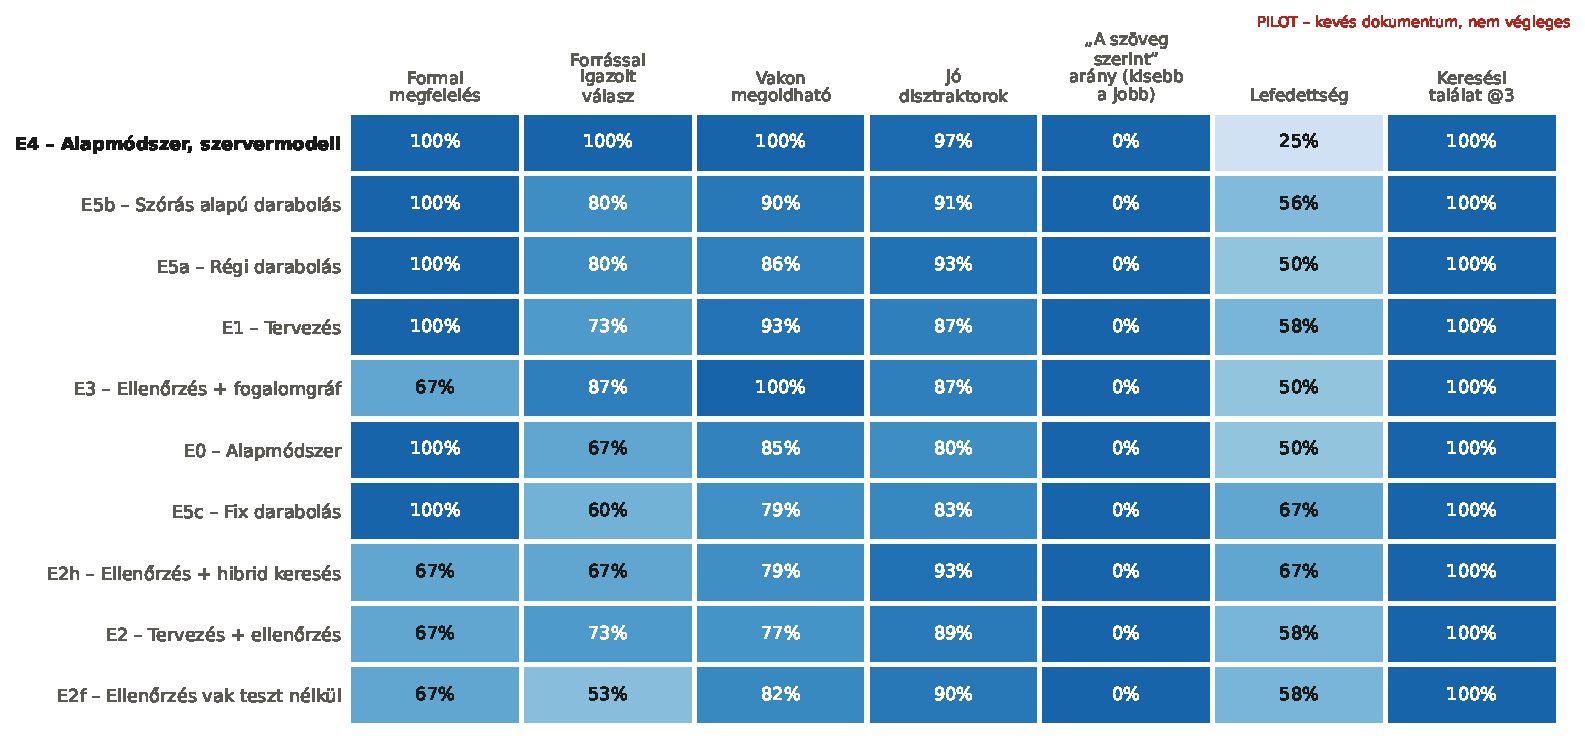
\includegraphics[width=\textwidth]{figures/abra3_mutatok.pdf}
\caption{Az egyes minőségi mutatók karonként (pilot). A „szöveg szerint” oszlop a meta-hivatkozások
aránya, a keresési találat@3 a referenciakérdések bizonyító mondatának visszakeresési aránya.}
\label{fig:mutatok}
\end{figure}

Három megfigyelés emelhető ki. \emph{Először}, a helyi karok minőségi indexe 0,73 és 0,90 között
szóródik, a szervermodell (\arm{E4}) pedig 0,99-cel kiemelkedik. \emph{Másodszor}, a tervezés
(\arm{E1}) a naiv alapvonalhoz képest minden tartalmi mutatón javított, az ellenőrző karok
(\arm{E2}, \arm{E2f}, \arm{E2h}, \arm{E3}) viszont a formai megfelelésben 67\,\%-ra estek vissza, ami a
$Q$ indexüket jelentősen lerontotta. \emph{Harmadszor}, a lefedettség a szervermodellnél a
legalacsonyabb (25\,\%): a legjobb minőségű kar a dokumentum négy darabjából egyre koncentrált. A
visszakeresési találati arány minden karon 100\,\% volt, ami egy négydarabos dokumentumon várható
(a három visszakeresett darab a négyből szinte mindig tartalmazza a bizonyítékot); a visszakeresés
mutatói csak a hosszú dokumentumokon lesznek informatívak.

\section{A tervezés hatása (RQ1, RQ2)}

A naiv alapvonal (\arm{E0}) és a tervezett, de nem ellenőrzött csővezeték (\arm{E1}) összevetése
(\ref{tab:pilot-fo}. és \ref{tab:rubrika-eredmeny}.~táblázat) szerint a tervezés azonos modell és azonos formai megfelelés mellett javította az alátámasztottságot
($+6$ százalékpont), a vak megoldhatóságot ($+8$), a disztraktor-validitást ($+7$) és a lefedettséget
($+8$), a bíró helyességi pontszámát 3,5-ről 3,7-re, disztraktorpontszámát 3,5-ről 4,0-ra, a
„felhasználnám” arányt 63-ról 67\,\%-ra emelte, az érthetőségi pontszám viszont 4,7-ről 4,0-ra csökkent. Az ára: 23-szoros hívásszám és
9-szeres futási idő (20 másodperc helyett 3 perc).


Az érthetőség csökkenése mögött a kérdések formájának megváltozása áll: az egyenkénti generálás
hosszabb törzseket és jóval hosszabb válaszlehetőségeket eredményezett (\ref{tab:hosszak}.~táblázat).
A naiv alapvonal egy vizsgán belül rövid, tényfelidéző kérdéseket írt, 60 karakteres átlagos
törzzsel és négy opcióra összesen 60 karakterrel („9. század”, „10. század”, \dots); a tervezett
csővezeték kérdései átlagosan 88 karakteres törzsűek, az opciók együttes hossza pedig 315 karakter,
vagyis tipikusan teljes mondatok. Ez a fogalmi, magyarázó kérdéseknek kedvez (a disztraktorpontszám
nőtt), de a kérdés olvasási terhét is növeli.

\begin{table}[htbp]
\centering
\caption{A kérdések hossza, változatossága és tematikus hasonlósága karonként (pilot, átlagok 30
kérdésen). Törzs: a törzs karakterszáma; Opciók: a négy opció együttes karakterszáma; Dup.: duplikátumráta;
RefSim: átlagos maximális hasonlóság a referenciakérdésekhez.}
\label{tab:hosszak}
\small
\begin{tabular}{@{}lrrcc@{}}
\toprule
Kar & Törzs & Opciók & Dup. (\%) & RefSim \\
\midrule
\arm{E0}  & 60  & 60  & 16 & 0,895 \\
\arm{E1}  & 88  & 315 & 21 & 0,912 \\
\arm{E2}  & 84  & 348 & 21 & 0,909 \\
\arm{E2f} & 95  & 405 & 17 & 0,911 \\
\arm{E2h} & 93  & 352 & 14 & 0,907 \\
\arm{E3}  & 120 & 365 & 25 & 0,895 \\
\arm{E4}  & 54  & 87  & 4  & 0,890 \\
\arm{E5a} & 65  & 88  & 16 & 0,898 \\
\arm{E5b} & 58  & 73  & 10 & 0,891 \\
\arm{E5c} & 57  & 36  & 45 & 0,885 \\
\bottomrule
\end{tabular}
\end{table}

A referenciakérdésekhez való hasonlóság (RefSim) a tervezett karokban a legmagasabb (0,907--0,912),
ami arra utal, hogy a tervező által választott fogalmak jobban egyeznek a szakértő által fontosnak
tartott tényekkel. A különbség azonban kicsi, és egyetlen dokumentumon nem értelmezhető
megbízhatóan.

\paragraph{A tervezett Bloom-szint és a megvalósult szint.} A könnyű vizsgaszinthez a terv
50--50\,\%-ban emlékezés és megértés szintű kérdéseket írt elő (\ref{tab:bloom}.~táblázat), a bíró
azonban az \arm{E1} kar 30 kérdéséből 29-et emlékezés szintűnek sorolt be (\arm{E2}: 28, \arm{E2h}: 24,
\arm{E3}: 30). A kis modell tehát a promptban megadott kognitív szintet nem valósítja meg
megbízhatóan: a „megértés” szintű slotokból is jellemzően tényfelidéző kérdés lett. A szintillesztési
pontszám ennek ellenére 5,0, mert a könnyű nehézséghez mindkét szint elfogadható. Ez a megfigyelés arra
utal, hogy a Bloom-szint mint szerkezeti garancia (\ref{all:kvota}.~állítás) csak a \emph{kért}
szintre vonatkozik; a megvalósult szint ellenőrzése egy további, eddig hiányzó ellenőrzési lépés
lenne.

\section{Az ellenőrzés hatása}
\label{sec:verifier-eredmeny}

\subsection{A formai hiba és a tartalékkérdés}
\label{sec:fallback}

Az ellenőrző karok mindegyikében (\arm{E2}, \arm{E2f}, \arm{E2h}, \arm{E3}) a három vizsgából egyben
előfordult, hogy egy slot minden kísérlete, a tartalékfogalommal végzett kísérleteket is beleértve,
elbukott, és a megtartott végső kérdésnek csak két vagy három válaszlehetősége volt. Ez a vizsga formai
megfelelését nullára, a minőségi indexét $0{,}25$-tel csökkentette -- a négy kar $Q$ indexének
csökkenése az \arm{E1}-hez képest nagyrészt ebből ered. A hiba nem a módszer elvi korlátja, hanem
implementációs hiányosság volt: a végső kérdés kiválasztása csak a hibák számát nézte, a formát nem. A
javítás \az{\eqref{eq:rank}} lexikografikus kulcs és a javító hívás (\ref{alg:slot}.~algoritmus); a fő
vizsgálat ezt már tartalmazza.

\subsection{Az ellenőrző mint osztályozó}

A formai hibától függetlenül az ellenőrzés a tartalmi mutatókon sem javított: a tervezésre épülő
ellenőrzés (\arm{E2}) alátámasztottsága az \arm{E1}-ével azonos (73\,\%), vak megoldhatósága pedig
93-ról 77\,\%-ra csökkent. Az ok megértéséhez az ellenőrzőt osztályozóként értékeltük
(\ref{tab:verifier-biro}. és \ref{tab:verifier-karok}.~táblázat).

\begin{table}[htbp]
\centering
\caption{Egyezik-e a 7B ellenőrző ítélete a bíróéval? Az \arm{E2}, \arm{E2f}, \arm{E2h} és \arm{E3}
karok pilot kérdései az ellenőrző ítélete szerint; a bírói kimenetek \%-ban.}
\label{tab:verifier-biro}
\small
\begin{tabular}{@{}lcccc@{}}
\toprule
Ellenőrző ítélete & $n$ & Alátámasztott & Vakon helyes & Felhasználnám \\
\midrule
Átengedett (ellenőrzött) & 67 & 66 & 89 & 61 \\
Megjelölt (nem ellenőrzött) & 53 & 75 & 79 & 64 \\
\bottomrule
\end{tabular}
\end{table}

\begin{table}[htbp]
\centering
\caption{Az ellenőrző pontossága, felidézése és Cohen-$\kappa$ együtthatója a bíró alátámasztottsági
ítéletéhez képest, karonként. Átengedett: az átengedett kérdések aránya (\%).}
\label{tab:verifier-karok}
\small
\begin{tabular}{@{}lccccc@{}}
\toprule
Kar & $n$ & Átengedett & Pontosság & Felidézés & $\kappa$ \\
\midrule
\arm{E2}  & 30 & 57 & 0,71 & 0,55 & $-0{,}07$ \\
\arm{E2f} & 30 & 67 & 0,50 & 0,62 & $-0{,}09$ \\
\arm{E2h} & 30 & 60 & 0,61 & 0,55 & $-0{,}14$ \\
\arm{E3}  & 30 & 40 & 0,92 & 0,42 & $0{,}07$ \\
\bottomrule
\end{tabular}
\end{table}

Az eredmény egyértelmű: az ellenőrző által \emph{átengedett} kérdéseket a bíró \emph{ritkábban}
(66\,\%) ítélte alátámasztottnak, mint a \emph{megjelölteket} (75\,\%); a vak megoldhatóságban az
átengedettek kissé jobbak (89 vs.\ 79\,\%), a „felhasználnám” arány pedig gyakorlatilag azonos. Az
ellenőrző $\kappa$ együtthatója minden karon $-0{,}14$ és $0{,}07$ között van, vagyis az ellenőrző
ítélete a véletlen egyezés szintjén áll. Az \arm{E3} kar magas pontossága (0,92) alacsony felidézéssel
párosul: az ellenőrző ott a kérdések 60\,\%-át megjelölte, és az átengedettek zöme valóban
alátámasztott volt -- ez azonban részben \az{\ref{sec:szivargas}}.~szakaszban tárgyalt szivárgásnak
köszönhető.

Az értelmezésünk szerint egy 7B modell, amely egyben a generátor is, nem tudja megbízhatóan eldönteni,
hogy egy szövegrész következményként tartalmaz-e egy állítást; az ellenőrzés így a generátorral
korrelált, nem független információforrás. Ez összhangban van azzal, hogy külső visszajelzés nélkül a
modellek önjavítása nem javít~\cite{huang2024selfcorrect}, és azzal, hogy a modellek saját kimenetüket
előnyben részesítik~\cite{panickssery2024selfpref}. Két következménye van a fő vizsgálatra: az
ellenőrző jelzését nem szabad az oktatónak megbízhatóságként bemutatni, amíg osztályozóként nem
validáltuk; és külön karban (\arm{E2x}) kell tesztelni, hogy egy másik modellcsaládba tartozó ellenőrző
független-e a generátortól.

\section{Válaszszivárgás: egy új hibamód}
\label{sec:szivargas}

A kérdések kézi átolvasása olyan hibát tárt fel, amelyet sem az automatikus mutatók, sem a bíró nem
büntetett: egyes ellenőrzött kérdések egy forrásmondatot másolnak a törzsbe, és ugyanazt a mondatot
ismétlik meg kulcsként. \Az{\ref{tab:szivargas}}.~táblázat a szivárgás gyakoriságát mutatja.

\begin{table}[htbp]
\centering
\caption{Válaszszivárgás karonként (pilot, 30 kérdés karonként, \%). Kulcs a törzsben: legalább
háromszavas kulcs, amelynek szótokenjei legalább 80\,\%-ban a törzsben is szerepelnek; nem kérdés: a
törzs sem kérdőjelre, sem kettőspontra nem végződik; bírói helyesség: a szivárgó kérdések átlagos
helyességi pontszáma (1--5).}
\label{tab:szivargas}
\small
\begin{tabular}{@{}lcccc@{}}
\toprule
Kar & $n$ & Kulcs a törzsben & Nem kérdés & Bírói helyesség (szivárgó) \\
\midrule
\arm{E0}  & 30 & 0  & 0  & -- \\
\arm{E1}  & 30 & 0  & 13 & -- \\
\arm{E2}  & 30 & 3  & 17 & 5,0 \\
\arm{E2f} & 30 & 7  & 10 & 5,0 \\
\arm{E2h} & 30 & 10 & 10 & 2,3 \\
\arm{E3}  & 30 & \textbf{20} & \textbf{47} & 5,0 \\
\arm{E4}  & 30 & 0  & 0  & -- \\
\arm{E5a} & 30 & 0  & 33 & -- \\
\arm{E5b} & 30 & 0  & 0  & -- \\
\arm{E5c} & 30 & 0  & 0  & -- \\
\bottomrule
\end{tabular}
\end{table}

A szivárgás kizárólag az ellenőrző karokban fordult elő, és ott a legerősebb, ahol a legtöbb
újrapróbálkozás történt (\arm{E3}: 20\,\% szivárgás, 47\,\% nem-kérdés törzs). A bíró a szivárgó kérdések
többségének 5-ös helyességi pontszámot adott, ami érthető: a kulcs valóban alátámasztott, hiszen
szó szerint a forrásból származik, és a kérdés „vakon” is megoldható, hiszen a válasz a kérdésben van. A
szivárgás tehát \emph{egyszerre} torzítja felfelé az alátámasztottságot, a vak megoldhatóságot és a
bírói pontszámot -- ez magyarázza, hogy az \arm{E3} kar miért érte el a legmagasabb helyi
alátámasztottságot (87\,\%) és vak megoldhatóságot (100\,\%).

Értelmezésünk szerint az ellenőrző visszacsatolási hurka a kis modellt a forrásszöveg szó szerinti
átvétele felé tolja, mert ez a legolcsóbb módja annak, hogy egy alátámasztottsági ellenőrzésen
átjusson. Ez a jelenség a Goodhart-törvény egy példája: a mérőszám célponttá válva elveszíti mérő
jellegét. A fő vizsgálatra két következménye van: a szivárgást és a nem-kérdés törzset az ellenőrző
lánc szabályként elutasítja (\ref{tab:checks}.~táblázat), és mindkettő mutatóként is szerepel minden
jelentésben.

\section{Szervermodell és helyi modell (RQ3)}

A nagy szervermodell naiv RAG-gal (\arm{E4}) minden tartalmi mutatón a legjobb volt: alátámasztottság
és vak megoldhatóság 100\,\%, disztraktor-validitás 97\,\%, a bíró minden kérdését felhasználná
(\ref{tab:rubrika-eredmeny}.~táblázat). A lefedettsége azonban a legalacsonyabb (25\,\%): mindhárom vizsgában az összes
kérdés a dokumentum négy darabja közül ugyanahhoz az egyhez állt a legközelebb. Ez a P2 probléma --
a kérdések egy szakaszra tömörülése -- kis léptékben: a nagyobb modell sem terjeszti szét magától a
kérdéseit, ha a feladat erre nem kényszeríti. A megosztott egyetemi szerveren a medián futási idő
6,6 perc volt vizsgánként, ugyanannyi, mint az ellenőrzött helyi csővezetéké (6,2 perc), miközben a helyi
naiv alapvonal 20 másodperc alatt végzett.

\begin{table}[htbp]
\centering
\caption{A bíró rubrikapontszámai (1--5, átlagok 30 kérdésen) és a „felhasználnám” arány karonként
(pilot).}
\label{tab:rubrika-eredmeny}
\small
\begin{tabular}{@{}lccccc@{}}
\toprule
Kar & Helyesség & Érthetőség & Disztraktorok & Szintillesztés & Felhasználnám \\
\midrule
\arm{E0} (naiv)            & 3,5 & 4,7 & 3,5 & 4,8 & 63\,\% \\
\arm{E1} (terv)            & 3,7 & 4,0 & 4,0 & 5,0 & 67\,\% \\
\arm{E2} (+ ellenőrzés)    & 3,4 & 4,1 & 3,6 & 5,0 & 60\,\% \\
\arm{E2f} (vak próba nélkül) & 3,1 & 4,0 & 4,0 & 4,9 & 50\,\% \\
\arm{E2h} (hibrid keresés) & 3,5 & 4,1 & 4,2 & 4,8 & 63\,\% \\
\arm{E3} (+ gráf)          & 4,4 & 4,4 & 3,9 & 5,0 & 77\,\% \\
\arm{E4} (szerver, naiv)   & \textbf{5,0} & \textbf{5,0} & \textbf{4,6} & 5,0 & \textbf{100\,\%} \\
\arm{E5a} (régi kódoló)    & 3,8 & 4,3 & 3,9 & 5,0 & 70\,\% \\
\arm{E5b} (szórásküszöb)   & 4,1 & 4,5 & 3,7 & 4,9 & 77\,\% \\
\arm{E5c} (fix darabok)    & 3,3 & 4,0 & 3,0 & 5,0 & 57\,\% \\
\bottomrule
\end{tabular}
\end{table}

A helyi modell erőforrásigényét \az{\ref{sec:vram}}.~szakasz részletezte: a modell és a futtatókörnyezet
5\,400--5\,950\,MiB-ot foglalt, a csúcs 7\,808\,MiB volt, így a helyi csővezeték egy 8\,GB-os kártyán az
asztali környezet mellett is fut. \Az{\ref{h:helyi}}.~hipotézis szerinti $<0{,}1$ különbséget a pilot
nem támasztja alá (\arm{E4}: 0,99; a legjobb tervezett helyi kar, \arm{E1}: 0,88), a legjobb egyhívásos
helyi karok (\arm{E5a}, \arm{E5b}: 0,90) azonban 0,09-re megközelítették.

\section{Költség}
\label{sec:koltseg}

\Az{\ref{tab:koltseg}}.~táblázat a hívásszámot szakaszonként, a tokenfelhasználást és a futási időt mutatja.
\Az{\ref{fig:minoseg-ido}}.~ábra a minőséget a futási idő függvényében ábrázolja.

\begin{table}[htbp]
\centering
\caption{Modellhívások szakaszonként, tokenfelhasználás és futási idő vizsgánként (pilot, átlagok 3
vizsgán; az idő medián). Terv.: tervező vagy gráfépítés; Gen.: generálás; Alát.: alátámasztottsági
ellenőrzés; Vak: vak megoldási ellenőrzés.}
\label{tab:koltseg}
\small
\begin{tabular}{@{}lrrrrrrr@{}}
\toprule
Kar & Terv. & Gen. & Alát. & Vak & Összes & Token (e) & Perc \\
\midrule
\arm{E0}  & -- & 1    & --   & --   & 1     & 2,8   & 0,3 \\
\arm{E1}  & 1  & 22,0 & --   & --   & 23,0  & 45,2  & 3,0 \\
\arm{E2}  & 1  & 31,0 & 29,0 & 14,3 & 75,3  & 96,7  & 6,2 \\
\arm{E2f} & 1  & 29,3 & 28,3 & --   & 58,7  & 84,1  & 5,3 \\
\arm{E2h} & 1  & 30,7 & 29,7 & 15,0 & 76,3  & 99,2  & 6,7 \\
\arm{E3}  & 1  & 43,7 & 37,3 & 18,7 & 100,7 & 119,6 & 8,0 \\
\bottomrule
\end{tabular}
\end{table}

\begin{figure}[htbp]
\centering
\begin{tikzpicture}
\begin{axis}[
  width=0.9\textwidth, height=7cm, xmode=log,
  xmin=0.2, xmax=12, ymin=0.68, ymax=1.03,
  xtick={0.25,0.5,1,2,4,8}, xticklabels={{0,25},{0,5},1,2,4,8},
  yticklabel style={/pgf/number format/.cd, fixed, precision=2, use comma},
  xlabel={Medián futási idő vizsgánként (perc, logaritmikus skála)}, ylabel={Minőségi index $Q$},
  xlabel style={font=\small}, ylabel style={font=\small},
  tick label style={font=\footnotesize}, grid=major, grid style={gray!20},
  nodes near coords, point meta=explicit symbolic,
  every node near coord/.style={font=\footnotesize, anchor=south west, inner sep=1.5pt},
  legend style={font=\footnotesize, at={(0.30,0.97)}, anchor=north west}]
\addplot[only marks, mark=*, mark size=2.4pt, blue!70!black] coordinates {
  (0.33,0.830) [E0] (2.98,0.881) [E1] (6.23,0.764) [E2] (5.29,0.731) [E2f]
  (6.72,0.765) [] (8.05,0.850) [E3] (0.35,0.899) [E5a] (0.29,0.806) [E5c]};
\addlegendentry{helyi 7B modell (RTX 3070 Ti)}
\addplot[only marks, mark=square*, mark size=2.4pt, orange!85!black] coordinates {(6.61,0.992) [E4]};
\addlegendentry{szervermodell (naiv RAG)}
\node[font=\footnotesize, anchor=west, blue!70!black] at (axis cs:7.0,0.748) {E2h};
\addplot[only marks, mark=*, mark size=2.4pt, blue!70!black, forget plot, every node near coord/.style={font=\footnotesize, anchor=north west, inner sep=1.5pt}] coordinates {(0.33,0.903) [E5b]};
\end{axis}
\end{tikzpicture}
\caption{Minőség és futási idő a pilotban. A tervezett karok egy nagyságrenddel lassabbak; a
minőségnövekedést csak a tervezés (\arm{E1}) hozta meg ellenőrzés nélkül.}
\label{fig:minoseg-ido}
\end{figure}

Az ellenőrző karok hívásszáma (59--101) messze meghaladja \az{\eqref{eq:callbounds}} szerinti alsó korlátot
(21--31), ami azt jelzi, hogy a kérdések jelentős része legalább egyszer elbukott. Az \arm{E2} kar
slotonként átlagosan 3,1 generálást igényelt; \az{\eqref{eq:expattempts}} képletet a tartalékfogalommal együtt
alkalmazva ez $p\approx0{,}3$ körüli kísérletenkénti átmenési valószínűségnek felel meg -- azaz a kis
modell ellenőrzője a kérdések kétharmadát első körben elutasította, miközben (az előző szakasz
szerint) ítélete a bíróéval nem egyezett. Az ellenőrzés tehát a pilotban a hívásszámot 60--100-szorosára
növelte anélkül, hogy információt adott volna. A tervezés (\arm{E1}) ezzel szemben 23 hívással mérhető
minőségjavulást hozott; a pilot alapján a fő vizsgálatban a tervezés bizonyítása, az ellenőrzés
pedig érdemének igazolása a feladat.

\section{Darabolási stratégiák}

Az egyhívásos alapvonalat három darabolási változattal is összevetettük (\ref{tab:pilot-fo}. és \ref{tab:hosszak}.~táblázat). A
rögzített, 800 karakteres ablakok (\arm{E5c}) adták a leggyengébb eredményt: a kérdéspárok 45\,\%-a
közel-duplikátum volt (a szemantikus darabolásnál 10--16\,\%), és a bíró disztraktorpontszáma 3,0-ra
esett (a szemantikus változatoknál 3,5--3,9). A szórásalapú küszöb (\arm{E5b}) és a régi kódoló
(\arm{E5a}) 0,90-es indexet ért el. Az utóbbi eredmény nem jelenti a régi kódoló előnyét: egy
512 tokennél rövidebb dokumentumon a régi és az új kódoló \emph{azonos} darabokat ad, így az \arm{E0}
és az \arm{E5a} közötti különbség kizárólag a futásról futásra jelentkező zajból ered.


\section{Futásról futásra jelentkező zaj}
\label{sec:zaj}

Az \arm{E0} és az \arm{E5a} kar a pilotban azonos darabokat, azonos visszakeresett kontextust és azonos
magokat kapott (ezt a nyers adatok, a \code{exams.jsonl} fájlok \code{retrieved} mezői igazolják),
mégis eltérő kérdéseket, és 0,83, illetve 0,90 minőségi indexet adtak. Ez a különbség tehát egy
természetes kontrollkísérlet: a teljes mérési láncot változatlanul hagyva, csak az ismétlés miatt
0,07-es eltérés adódott. Az ok az, hogy a GPU-n végzett következtetés alacsony hőmérsékleten és rögzített
maggal sem bitre reprodukálható (a párhuzamos lebegőpontos redukciók sorrendje nem determinisztikus).

Ebből két következtetés adódik. \emph{Egyrészt}, egyetlen dokumentumon a 0,07-nél kisebb különbségek
zajnak tekintendők -- a pilot szinte minden helyi karpárjának különbsége ebbe a sávba esik, a tervezés
hatása ($+0{,}05$) is. \emph{Másrészt}, a zaj csökkentésének hatékony módja nem a magok számának
növelése egyetlen dokumentumon, hanem a dokumentumok számának növelése, mert a fő vizsgálat
hipotézisei dokumentumok populációjára vonatkoznak. A fő vizsgálat ezért 39 dokumentumon,
dokumentumszintű statisztikával fut.

\section{Példák}

\Az{\ref{tab:peldak}}.~táblázat négy pilotkérdést mutat eredeti, magyar nyelvükön, a bíró ítéletével. A
példák a fenti eredmények tipikus eseteit illusztrálják: a naiv alapvonal téves kulcsát, a tervezett
kar alá nem támasztott részletét, a szivárgó kérdést és a szervermodell jó kérdését.

\begin{table}[htbp]
\centering
\caption{Pilotkérdések eredeti nyelven (* = megjelölt kulcs), a bíró ítéletével.}
\label{tab:peldak}
\footnotesize
\begin{tabularx}{\textwidth}{@{}>{\raggedright\arraybackslash}p{1.2cm}>{\raggedright\arraybackslash}X@{}}
\toprule
\arm{E0} & \emph{A kávé felfedezéséhez milyen században jutott el a velencei kereskedők révén?}
9.~század* / 10.~század / 8.~század / 11.~század. \textbf{Bíró:} nem alátámasztott -- a forrás szerint a
kávé a 17.~században jutott el Velencébe; a 9.~század az etióp legenda ideje. Egyik opció sem helyes;
helyesség 1/5. \\
\midrule
\arm{E1} & \emph{A pörkölés hőmérsékeltségének milyen hatással van az italt és a koffeintartalomra?}
Kulcs: \emph{A sötét pörkölés testesebb, füstösebb és keserűbb ízvilágot eredményez, de a
koffeintartalom csökken.}* \textbf{Bíró:} az ízhatást a forrás igazolja, a koffeintartalomról azonban nem
szól, így a kulcs nem alátámasztott; a disztraktorok jók; helyesség 1/5. (A törzs nyelvtani hibája a 7B
modell magyar nyelvi korlátját is mutatja.) \\
\midrule
\arm{E3} & \emph{„A kávéfogyasztás szokása Etiópiából hamar átterjedt a szomszédos Jemenbe, majd az arab
világba, Európába pedig a 17.~században jutott el a velencei kereskedők révén.”} Kulcs: ugyanez a
mondat*; disztraktorok: a mondat a 16., 18., illetve 15.~századdal. \textbf{Bíró:} alátámasztott, vakon
helyes, helyesség 5/5 -- noha a „törzs” nem kérdés, és a választ szó szerint tartalmazza. \\
\midrule
\arm{E4} & \emph{Mennyit tesz ki az Arabica a globális kávétermelésből?} Mintegy 70 százalékát* /
Mintegy 30 százalékát / Mintegy 50 százalékát / Mintegy 90 százalékát. \textbf{Bíró:} a forrás a 70\,\%-ot
közvetlenül kimondja; a többi arány hihető, de a szöveg cáfolja; helyesség 5/5. \\
\bottomrule
\end{tabularx}
\end{table}

\section{A hipotézisek előzetes értékelése}

\Az{\ref{tab:hipotezisek}}.~táblázat összefoglalja, hogy a pilot milyen irányú bizonyítékot szolgáltat az
egyes hipotézisekhez. Hangsúlyozzuk, hogy ezek egyetlen dokumentumon, szignifikanciavizsgálat nélkül
tett, leíró megfigyelések; a hipotézisek eldöntése a fő vizsgálat feladata.

\begin{table}[htbp]
\centering
\caption{A hipotézisek és a pilot által szolgáltatott előzetes, leíró bizonyíték.}
\label{tab:hipotezisek}
\small
\begin{tabularx}{\textwidth}{@{}>{\raggedright\arraybackslash}p{2.6cm}>{\raggedright\arraybackslash}X>{\raggedright\arraybackslash}p{2.6cm}@{}}
\toprule
Hipotézis & Pilot megfigyelés & Irány \\
\midrule
\ref{h:terv}.\ Tervezés & alátámasztottság $+6$, lefedettség $+8$ pp, forma változatlan; a különbség a zajsávon belül & támogató, nem döntő \\
\ref{h:verif}.\ Ellenőrzés & alátámasztottság változatlan, vak megoldhatóság $-16$ pp; $\kappa\in[-0{,}14;0{,}07]$ & ellentmondó (önellenőrzésre) \\
\ref{h:lefed}.\ Lefedettség & a szervermodell naiv RAG-gal 25\,\% lefedettséget ért el; a \arm{B-doc} kar még nem futott & támogató (közvetett) \\
\ref{h:helyi}.\ Helyi vs.\ szerver & különbség 0,09--0,11; memória 5,4--5,9\,GiB & részben támogató \\
\ref{h:meres}.\ Mérés & oktatói értékelés még nincs; a bíró a szivárgó kérdéseket nem büntette & nyitott; kockázat azonosítva \\
\bottomrule
\end{tabularx}
\end{table}

\section{A fő vizsgálat eredményei}
\label{sec:fo-vizsgalat}

A fő vizsgálat (\code{eval-v1}, 39 dokumentum, \az{\ref{tab:karok}}.~táblázat összes kara, oktatói
értékeléssel) futása e dolgozat lezárásakor folyamatban van. Eredményei a keretrendszer
\code{report} lépésével, a pilottal azonos formában, automatikusan kerülnek \az{\ref{tab:fo-vizsgalat}}.~táblázatba és a hozzá tartozó szignifikanciatáblába. A táblázat szerkezetét
itt rögzítjük; a piros mezők a fő futás adataira várnak.

\begin{table}[htbp]
\centering
\caption{A fő vizsgálat eredményei (39 dokumentum; átlag és 95\,\%-os bootstrap-CI; páros
Wilcoxon-próba Holm-korrekcióval a referenciakarhoz képest). \tbd{A fő futás után kitöltendő.}}
\label{tab:fo-vizsgalat}
\small
\begin{tabular}{@{}llccccc@{}}
\toprule
Kar & Ref. & $Q$ [95\,\% CI] & Alát. & Lef. & $\tilde p$ (Holm) & $r_{rb}$ \\
\midrule
\arm{B-doc-L} & -- & \tbd{--} & \tbd{--} & \tbd{--} & -- & -- \\
\arm{E0}  & -- & \tbd{--} & \tbd{--} & \tbd{--} & -- & -- \\
\arm{E1}  & \arm{E0} & \tbd{--} & \tbd{--} & \tbd{--} & \tbd{--} & \tbd{--} \\
\arm{E2}  & \arm{E1} & \tbd{--} & \tbd{--} & \tbd{--} & \tbd{--} & \tbd{--} \\
\arm{E2x} & \arm{E2} & \tbd{--} & \tbd{--} & \tbd{--} & \tbd{--} & \tbd{--} \\
\arm{E3}  & \arm{E2} & \tbd{--} & \tbd{--} & \tbd{--} & \tbd{--} & \tbd{--} \\
\arm{E4}  & \arm{E0} & \tbd{--} & \tbd{--} & \tbd{--} & \tbd{--} & \tbd{--} \\
\arm{E4b} & \arm{E2} & \tbd{--} & \tbd{--} & \tbd{--} & \tbd{--} & \tbd{--} \\
\arm{B-doc-S} & -- & \tbd{--} & \tbd{--} & \tbd{--} & -- & -- \\
\bottomrule
\end{tabular}
\end{table}

% =====================================================================
\chapter{Diszkusszió}
\label{ch:diszkusszio}
% =====================================================================

\section{Miért módszer, és nem prompt?}

A dolgozat központi állítása, hogy a vizsgagenerálás megbízhatóságát nem egy jobb prompt, hanem a
feladat explicit, ellenőrizhető lépésekre bontása biztosítja. A két vizsgálat együtt négy ponton
támasztja alá ezt az érvelést. \emph{Először}, ugyanaz a 7B modell a tervezés és az ellenőrzés hatására
a fő vizsgálat hat dokumentumán a naiv RAG $0{,}64$-es és a teljes dokumentumos prompt $0{,}83$-as
indexéről $0{,}96$-ra javult, és elérte a teljes dokumentumot kapó szervermodellt ($0{,}95$); a különbség
nem a modell tudásából, hanem a feladat szerkezetéből ered. \emph{Másodszor}, a naiv RAG minősége a
darabolás apró részleteitől függött (az angol dokumentumokon $0{,}40$-re esett), a tervezett csővezetéké
nem: a fogalmanként végzett keresés robusztusabb, mint egy feladatleírással végzett keresés.
\emph{Harmadszor}, a kérdésenkénti forráshivatkozás lehetővé tette, hogy egy olvasó -- a kiértékelésben a
bíró, a gyakorlatban az oktató -- minden kulcsot a saját forrásával szemben ellenőrizzen; éppen ez tárta
fel a naiv alapvonal hibás kulcsait, az ellenőrző karok szivárgó kérdéseit és a szervermodell forma
szerint triviális kérdéseit. \emph{Negyedszer}, ugyanaz a csővezeték a nagy szervermodellel $0{,}99$-et ért
el: a módszer nem a kis modell mankója, hanem modelltől független keret.

A vizsgálatok a módszer határait is megmutatták. Az ellenőrzés a pilotban rontott, a fő vizsgálatban mind
a hat dokumentumon javított; a fordulatot a tartalékkérdés javítása és a szivárgási szabályok hozták, vagyis
az ellenőrzés haszna az implementáció részletein múlik. Az ellenőrző ítélete a bíróéval továbbra is csak
gyengén egyezik ($\kappa\le0{,}22$): a lánc a vizsga egészét javítja, de az egyes kérdésekre adott jelzése
nem megbízható. A pilot után megfogalmazott alternatíva -- ha a más modellcsaládba tartozó ellenőrző sem
független a generátortól, a helyi telepítés helyes konfigurációja az ellenőrzés nélküli \arm{E1} -- a fő
vizsgálat alapján módosul: a javasolt helyi konfiguráció az önellenőrző \arm{E2}, a megjelölést pedig
figyelmeztetésként, nem ítéletként kell az oktatónak megmutatni. A Llama-ellenőrző (\arm{E2x}) engedékenyebb
és lassabb, a fogalomgráf (\arm{E3}) és a hibrid keresés (\arm{E2h}) nem javított, így a jelen adatokon
egyik sem éri meg a többletköltségét. Végül a teljes dokumentumot kapó szervermodell a vizsgált,
többnyire rövid dokumentumokon sem minőségben, sem lefedettségben nem maradt el: a módszer előnye vele
szemben nem a rövid dokumentumokon mért minőség, hanem az ellenőrizhetőség, az adatvédelem és a helyi
futtathatóság (P1, P3, P4), a lefedettségi előny (P2) pedig a naiv RAG-gal szemben mutatható ki.

\section{A mérés mint kutatási eredmény}

A pilot talán legfontosabb eredménye módszertani: a mérés három különböző ponton torzított volna,
ha nem validáljuk. A tartalékvizsga-hiba a generálási sikert, a csonkolt kódoló a darabolás
minőségét, a szivárgás pedig a tartalmi mutatókat és a bíró ítéletét torzította -- mindhárom
esetben \emph{felfelé}, vagyis jobb eredményt mutatva a valósnál. A három hiba közös vonása, hogy a
mérőrendszer „működött”: nem adott hibaüzenetet, és hihető számokat állított elő. Ebből az a
módszertani tanulság következik, hogy a nyelvi modellekre épülő rendszerek kiértékelésében a nyers
kimenetek kézi átolvasása és a mutatók szélsőértékeinek tudatos vizsgálata nem helyettesíthető
automatizmussal; a mi esetünkben a legjobb helyi alátámasztottsági értéket (\arm{E3}, 87\,\%) éppen
egy hibamód okozta.

A futásról futásra jelentkező zaj ($\approx0{,}07$) becslése hasonló tanulság: a kevés dokumentumon,
kevés ismétléssel mért különbségek jelentős része zaj lehet.

A fő vizsgálat a bíróval kapcsolatban két újabb vakfoltot tárt fel. A teljes dokumentumos karoknál a bíró
24\,000 karakteres ablaka a hosszú dokumentumok végéről írt helyes kérdéseket „alá nem támasztottnak”
minősíti, ami ezeket a karokat lefelé torzítja; a szervermodell visszakeresett szakaszcímre vonatkozó,
tartalmilag üres kérdéseit („hány szóból áll a cím?”) pedig a bíró hibátlannak ítélte, ami felfelé torzít.
Egy harmadik tanulság a jelentés automatizmusára vonatkozik: a jelentésgenerátor a legmagasabb indexű
kart (\arm{E4b}) „győztesnek” jelölte, holott az más dokumentumokon futott, mint a többi kar. A futásonként
eltérő dokumentumhalmazt a nézőfelület figyelmeztetésként jelzi, a rangsor azonban csak azonos
dokumentumokon futott karok között értelmes.

\section{Az érvényességet veszélyeztető tényezők}
\label{sec:validitas}

A tapasztalati szoftvertechnológiai kutatás szokásos felosztását~\cite{wohlin2012experimentation}
követve négy érvényességi dimenziót vizsgálunk.

\paragraph{Belső érvényesség.} Az egytényezős kísérleti terv a karok közötti különbséget egyetlen
tényezőhöz köti, ám a tényezők nem mindig függetlenek: az ellenőrzés például a kérdések hosszát és
formáját is megváltoztatja, ami közvetve hat a bíró érthetőségi ítéletére. A GPU-következtetés
nemdeterminisztikussága miatt azonos konfiguráció mellett is eltérő kimenetek születnek; ezt a
dokumentumszintű aggregálás és a dokumentumok számának növelése kezeli. A pilot és a fő vizsgálat
között a csővezeték változott (szivárgási szabályok, javító hívás, $r=1$), így a két vizsgálat
eredményei nem közvetlenül összevethetők; a pilot eredményei az akkori implementációra vonatkoznak. A
fő vizsgálatban az \arm{E4} és az \arm{E4b} kar más dokumentumokon futott, mint a többi, ezért ezeket csak a
közös három dokumentumon vetjük össze; a tervezett karok egyetlen maggal futottak, így a dokumentumonkénti
értékükben a futásról futásra jelentkező zaj is benne van.

\paragraph{Konstrukciós érvényesség.} A minőségi index négy egyenlő súlyú komponense közül a formai
megfelelés vizsgaszintű bináris változó, a másik három kérdésszintű ráta; ezért egyetlen formai hiba
aránytalanul nagy hatású. Ezt tudatosan vállaljuk (egy hibás formájú kérdés a gyakorlatban
használhatatlanná teszi a vizsgát), de minden komponenst külön is közlünk. A lefedettség az
embedding-térbeli legközelebbi darabra épül, ami csak közelítése annak, hogy a kérdés „miről szól”.
Az alátámasztottság és a vak megoldhatóság a bíró ítéletén alapul; a bíró a kérdés kontextusát látja,
így a dokumentum más részeiben lévő ellentmondást nem veheti észre, és -- amint a szivárgás
megmutatta -- a formailag hibás, de „igaz” kérdéseket nem bünteti; a fő vizsgálat szerint a forma
szerint triviális kérdéseket sem, a teljes dokumentumos karoknál pedig legfeljebb a dokumentum első
24\,000 karakterét látja. A bíró validálása az oktatói értékeléssel ezért elengedhetetlen; a fő vizsgálat
lezárásakor az oktatói értékelés még nem érkezett be (\tbd{kitöltendő}), így a tartalmi mutatók egyelőre
egyetlen, nem validált bíróra épülnek.

\paragraph{Külső érvényesség.} A pilot egyetlen rövid, könnyű magyar szövegen futott, amelyen a naiv
alapvonal a négy darabból hármat lát -- ez a tervezés számára a legkedvezőtlenebb helyzet. A fő vizsgálat
a 39 dokumentumból kilencen futott (karonként hat); magyar részhalmaza három rövid saját szöveg, a
Wikipédia-cikkek egyike sem szerepelt benne, így a nyelv hatása a forrás és a hossz hatásával keveredik, és
az eredmények a teljes adatkészleten módosulhatnak. A vizsgált dokumentumok többsége rövid, ezért a
hosszú dokumentumokra jellemző jelenségek (a kontextus közepének gyengébb kihasználása, a csonkolás)
csak egy-két dokumentumon jelenhettek meg. Csak
feleletválasztós kérdéseket értékelünk; az igaz--hamis és a kifejtős kérdések minősége külön vizsgálatot
igényel. Az eredmények a vizsgált modellekre (Qwen2.5-7B, Llama-3.1-8B, a szervermodell) vonatkoznak;
egy másik modellcsalád eltérően viselkedhet.

\paragraph{Következtetési érvényesség.} A dokumentumszintű nemparaméteres tesztek konzervatívak.
A fő vizsgálat karonként hat dokumentuma éppen az a legkisebb szám, amelyen $p<0{,}05$ egyáltalán
elérhető; a hat összevetés közül egy (\arm{E2}--\arm{E1}) érte el, a Holm-korrekció után egyik sem. A
fő vizsgálat következtetései ezért leíró jellegűek; a 39 dokumentum közepes hatásméretek kimutatására
elegendő lenne, kis hatások kimutatására nem. A több
összehasonlítást Holm-korrekcióval kezeljük. A bootstrap-intervallumok kis mintán alulfedhetnek, ezért a
pontbecslések mellett mindig a dokumentumszintű eloszlást is közöljük.

\section{Etikai és jogi megfontolások}

A rendszer hallgatói adatot nem kezel, a feltöltött dokumentumok a feladat végén törlődnek
(\ref{sec:zero}.~szakasz), minden generált kérdés oktatói jóváhagyást igényel, az export pedig feltünteti
az MI-közreműködést és a modellt~\cite{aiact2024}. A kiértékelő dokumentumok saját vagy nyílt licencű
(CC BY 4.0, CC BY-SA 4.0) művek; a szerverkarok és a bíró az egyetem saját GenAI-infrastruktúráján futnak.
A rendszer célja a vázlatírás gyorsítása és ellenőrizhetővé tétele, nem az oktatói döntés kiváltása.

% =====================================================================
\chapter{Összefoglalás és további munka}
\label{ch:osszefoglalas}
% =====================================================================

\section{Összefoglalás}

Dolgozatunkban a vizsgakérdés-generálás négy gyakorlati problémájából indultunk ki: a kulcsok
helyessége nincs ellenőrizve (P1), a vizsga szerkezete és lefedettsége nincs kontrollálva (P2), a
tananyag egy harmadik félhez kerül (P3), és a módszer nagy, távoli modellekre támaszkodik (P4). Ezekre a
\Mimir{} rendszerrel válaszoltunk, amely az egyetlen promptot explicit, ellenőrizhető módszerrel váltja
fel, és egyetlen fogyasztói GPU-n, adatmegőrzés nélkül fut.

A munka eredményei a következőkben foglalhatók össze.

\begin{enumerate}[label=(\arabic*)]
\item \textbf{Formális modell.} A „jó vizsga” fogalmát mérhető, forrásalapú predikátumokra bontottuk
(formai helyesség, alátámasztottság, disztraktor-validitás, vak megoldhatóság, lefedettség,
szivárgás), a generálást korlátos optimalizálási feladatként írtuk fel, és bizonyítottuk a vizsgaterv
két szerkezeti tulajdonságát: a Bloom-kiosztás kvótatulajdonságát és a mohó slotkiosztás
lefedettségi alsó korlátját.
\item \textbf{Generálási módszer.} Kidolgoztuk és implementáltuk a tervezésvezérelt, forráshivatkozásos
csővezetéket: ablakozott szemantikus darabolás, lefedettségvezérelt vizsgaterv, slotonkénti sűrű vagy
hibrid visszakeresés, egyenkénti forráshoz kötött generálás, legolcsóbbtól a legdrágábbig rendezett
ellenőrző lánc visszacsatolással, tartalékfogalmakkal és javító hívással, valamint munkamenet-hatókörű
fogalomgráf.
\item \textbf{Adatvédő architektúra.} A mikroszolgáltatás-architektúra zéró adatmegőrzéssel,
ujjlenyomatokra épülő naplózással és kapcsolható, kizárólag helyi üzemmóddal működik; a GPU-memóriaigény
analitikus modelljét mérésekkel validáltuk: a 7B generátor és futtatókörnyezete 5,4--5,9\,GiB-ot foglal,
így 8\,GB-os kártyán is fut.
\item \textbf{Kiértékelési módszertan.} Tizenöt egytényezős kísérleti kart, 39 dokumentumos kétnyelvű
adatkészletet 326 referenciakérdéssel, modellcsaládon kívüli bírót, közös bíró--oktató rubrikát és
dokumentumszintű statisztikát tartalmazó, nyílt és reprodukálható keretrendszert hoztunk létre.
\item \textbf{Pilot eredmények.} Egyetlen dokumentumon a tervezés javította a helyi modell
alátámasztottságát, vak megoldhatóságát, disztraktorait és lefedettségét; az azonos modellel végzett
önellenőrzés a bíróval csak véletlenszintű egyezést mutatott; a visszacsatolási hurok a kulcs kérdésbe
szivárgását idézte elő, amely az automatikus mutatókat és a bírót egyaránt félrevezette; a futásról
futásra jelentkező zaj ($\approx0{,}07$) pedig megmutatta, hogy egyetlen dokumentumon a legtöbb különbség
nem értelmezhető. Ezekből a megfigyelésekből közvetlenül következtek a fő vizsgálat javításai.
\item \textbf{A fő vizsgálat eredményei.} Tizennégy karral, kilenc magyar és angol dokumentumon
(karonként hat), 1\,670 kérdésen: a helyi 7B modellel futó tervezett és ellenőrzött csővezeték érte el a
legmagasabb minőségi indexet a közös dokumentumokon ($0{,}96$), szemben a naiv RAG $0{,}64$-es, a helyi teljes
dokumentumos prompt $0{,}83$-as és a teljes dokumentumot kapó szervermodell $0{,}95$-ös értékével; a tervezés
$+0{,}24$-dal, az ellenőrzés -- a pilottal ellentétben -- mind a hat dokumentumon, $+0{,}08$-dal javított; a
más modellcsaládba tartozó ellenőrző és a fogalomgráf rontott; a szivárgási szabályok a szivárgást
0--3\,\%-ra szorították le; a naiv RAG az angol dokumentumokon a rövid szerkezeti darabok miatt összeomlott;
ugyanaz a csővezeték a szervermodellel $0{,}99$-et ért el. A Holm-korrekció után egyik összevetés sem
szignifikáns.
\end{enumerate}

A kutatási kérdésekre a két vizsgálat alapján a következő válaszokat adhatjuk. \textbf{RQ1:} a strukturált
generálás a vizsgált dokumentumokon érvényesebb vizsgát adott, mint ha ugyanannak a modellnek a dokumentumot
vagy annak visszakeresett részleteit egyetlen promptban adjuk át ($0{,}96$ vs.\ $0{,}83$ és $0{,}64$), és a
lefedettsége jobb volt a naiv RAG-énál; a teljes dokumentumos promptnál azonban nem volt jobb a lefedettsége
(\ref{h:lefed}.~hipotézis nem teljesült). \textbf{RQ2:} a tervezés 17 hívásért, az ellenőrzés további
34 hívásért javított, a vak megoldási próba a lánc hasznos eleme; a más modellcsaládba tartozó ellenőrző,
a fogalomgráf és a hibrid keresés a többletköltségéért nem javított; a naiv RAG-ot a darabolás apró
részletei is jelentősen befolyásolták. \textbf{RQ3:} a helyi 7B modell a tervezett és ellenőrzött
csővezetékben a közös dokumentumokon elérte a szervermodell naiv RAG-os ($0{,}95$ vs.\ $0{,}93$) és teljes
dokumentumos ($0{,}96$ vs.\ $0{,}95$) változatát, a pilotban mért 5,4--5,9\,GiB GPU-memóriával; ugyanazzal a
csővezetékkel a szervermodell $0{,}99$-et ért el, vizsgánként 47,7 perc alatt.

\section{További munka}

A közvetlen folytatás a fő vizsgálat kiterjesztése \az{\ref{ch:kiertekeles}}.~fejezetben rögzített
protokoll szerint: a fő karok (\arm{B-doc-L}, \arm{B-doc-S}, \arm{E0}, \arm{E1}, \arm{E2}, \arm{E4},
\arm{E4b}) futtatása mind a 39 dokumentumon, köztük a 24 magyar Wikipédia-cikken, azonos dokumentumokon
a helyi és a szerverkarokkal; a bíró validálása három oktató vak értékelésével; és a bíró kontextusablakának
bővítése a teljes dokumentumos karokra. Ezen túl a következő irányokat tartjuk ígéretesnek.

\begin{itemize}
\item \textbf{Minimális darabméret.} A naiv RAG angol dokumentumokon mért összeomlását a szerkezeti
sorokból képzett, tartalom nélküli darabok okozták; a darabolóba illesztett minimális darabméret (a rövid
darab összevonása a szomszédjával) egyszerű javítás, amelynek hatása egy újabb \arm{E0}-futással mérhető.
\item \textbf{Megbízhatóbb ellenőrző.} Az ellenőrzés javítja a vizsgát, de a kérdésenkénti jelzése a bíróval
csak gyengén egyezik, és a más modellcsaládba tartozó ellenőrző (\arm{E2x}) sem jobb. Természetes nyelvi
következtetésre (NLI) tanított kisebb osztályozó vagy a FActScore-hoz hasonló atomi
tényellenőrzés~\cite{min2023factscore} lehet a következő lépés.
\item \textbf{A megvalósult Bloom-szint ellenőrzése.} A pilot szerint a kis modell a kért kognitív
szintet nem valósítja meg megbízhatóan; egy szintosztályozó ellenőrzés az ellenőrző láncba illeszthető.
\item \textbf{Adaptív ellenőrzés.} Az ellenőrzés költségét csökkentené, ha csak a bizonytalan
kérdésekre futna (pl.\ a kulcs lexikális alátámasztottsága vagy a generátor bizonyossága alapján).
\item \textbf{Nyelvi összevetés.} Az angol dokumentumok egy részének magyar fordítása lehetővé tenné a
nyelv hatásának a forrástól független mérését.
\item \textbf{További kérdéstípusok és tanórai kipróbálás.} Az igaz--hamis és a kifejtős kérdések
kiértékelése, valamint a generált vizsgák pszichometriai elemzése (nehézségi és diszkriminációs index,
nem funkcionáló disztraktorok) valós hallgatói válaszokon.
\end{itemize}

A \Mimir{} nyílt forráskódú: a kód, a konfigurációk, az adatkészlet-manifesztek, a pilot nyers
kimenetei és a fő vizsgálat jelentése a reprodukáláshoz rendelkezésre állnak.


% ----------------------------- JEGYZÉKEK -----------------------------
\cleardoublepage
\begin{singlespace}
\printbibliography[heading=bibintoc,title={Irodalomjegyzék}]
\end{singlespace}

\cleardoublepage
\phantomsection
\addcontentsline{toc}{chapter}{Ábrajegyzék}
\begin{singlespace}
\listoffigures
\end{singlespace}

\cleardoublepage
\phantomsection
\addcontentsline{toc}{chapter}{Táblázatjegyzék}
\begin{singlespace}
\listoftables
\end{singlespace}

% ----------------------------- FÜGGELÉK ------------------------------
\appendix
% =====================================================================
%  Függelékek
% =====================================================================

\chapter{Promptok}
\label{app-prompt}

Ez a függelék a csővezetékek promptjait közli (rövidítve, a JSON-sémák elhagyásával ott, ahol a
törzsszövegből egyértelműek). A belső lépések (tervező, gráf, ellenőrző) promptjai angol nyelvűek,
mert a kis helyi modellek ezeket megbízhatóbban követik; a generátor promptja magyar, és megismétli az
éles prompt szabályait, így az \arm{E0} és az \arm{E1+} karok szerkezetben, nem szabályokban
különböznek.

\section{A naiv alapvonal (\arm{E0}) és a teljes dokumentumos alapvonal promptja}
\begin{lstlisting}
Te egy kiemelkedő tudású oktatásmódszertani szakértő és professzionális vizsgakészítő vagy.

KÖTELEZŐ SZABÁLYOK, AMIKET SZIGORÚAN BE KELL TARTANOD:
1. ZÉRÓ HALLUCINÁCIÓ: KIZÁRÓLAG a megadott KONTEXTUS alapján dolgozz! Ha a kontextus nem
   tartalmazza a választ, ne találj ki semmit!
2. FELHASZNÁLÓI UTASÍTÁS KÖVETÉSE: ... Pontosan a kért mennyiséget és típust generáld le!
3. DISZTRAKTOROK: Feleletválasztós (mcq) kérdés esetén 1 helyes és 3 hihető, de helytelen válasz.
4. NO LATEX: Szigorúan TILOS LaTeX formázást vagy dollárjeleket ($) használni!
5. META-REFERENCIA TILALOM: Szigorúan TILOS a dokumentum szerkezetére kérdezni.

KONTEXTUS:
{context_text}

FELADAT (A felhasználó pontos kérése):
"{query}"

KIMENETI FORMÁTUM: kizárólag egy érvényes JSON objektum:
{"title": "Mimir AI Vizsga", "format": "pdf", "questions": [
  {"type": "mcq", "text": "...?", "answers": [{"text": "...", "is_correct": true}, ...]}]}
\end{lstlisting}

\section{A tervező promptja}
\begin{lstlisting}
[planner] You design exam blueprints. Reply with one valid JSON object only.

Below is a document split into numbered chunks (C0, C1, ...). Some chunks are shortened.
{overview}
List the {n_concepts} most important, clearly distinct concepts, facts or ideas a student should
be tested on. Cover the whole document: every major part should have at least one concept. Prefer
central ideas over trivia. Write concept names and descriptions in {language}.
JSON shape:
{"concepts": [{"concept": "short name", "description": "one sentence: what exactly should be
  tested", "chunk_ids": ["C0"], "importance": 3}]}
importance: 3 = central, 2 = important, 1 = detail.
\end{lstlisting}

\section{A generátor promptja}
\begin{lstlisting}
[generator] Te egy kiemelkedő tudású oktatásmódszertani szakértő és professzionális vizsgakészítő
vagy. Kizárólag érvényes JSON formátumban válaszolj, markdown formázás nélkül!

Készíts PONTOSAN EGY vizsgakérdést az alábbi terv szerint.
TERV:
- Fogalom: {concept}
- Mit kérdezzen: {description}
- Kérdéstípus: feleletválasztós ("mcq"): pontosan 4 válasz, ebből pontosan 1 helyes és 3 hihető,
  de a kontextus szerint egyértelműen helytelen disztraktor; a válaszok hossza és formája legyen
  hasonló.
- Bloom-szint: {pl. Megértés (magyarázat, összehasonlítás, saját szavakkal)}
- Vizsga nehézsége: {difficulty}
- Nyelv: a kérdést és a válaszokat {magyar} nyelven írd.
KÖTELEZŐ SZABÁLYOK:
1. ZÉRÓ HALLUCINÁCIÓ: KIZÁRÓLAG a KONTEXTUS alapján dolgozz. A helyes válasznak a kontextusból
   igazolhatónak kell lennie.
2. HIVATKOZÁS: a "citations" mezőbe írd azoknak a részleteknek az azonosítóját (pl. "C3"),
   amelyek igazolják a helyes választ.
3. NO LATEX.  4. META-REFERENCIA TILALOM.
5. NE ISMÉTELD a már elkészült kérdéseket: {existing}
[DISZTRAKTOR-ÖTLETEK (rokon fogalmak a dokumentumból) - csak E3]
[AZ ELŐZŐ PRÓBÁLKOZÁS HIBÁS VOLT, JAVÍTSD: {feedback}]
KONTEXTUS:
[C3] ...
[C1] ...
KIMENETI FORMÁTUM (csak ez a JSON objektum):
{"type": "mcq", "text": "A kérdés szövege?", "answers": [...], "citations": ["C0"],
 "bloom": "understand", "explanation": "egy mondat: miért ez a helyes válasz"}
\end{lstlisting}

\section{Az ellenőrző promptjai}
\begin{lstlisting}
[verifier] You check exam questions against source text. Reply with one valid JSON object only.

SOURCE: """{source}"""
QUESTION (mcq): {text}
A. ...   <-- marked correct
B. ...
Check strictly against the SOURCE only:
1. key_supported: is the marked-correct answer clearly supported by the SOURCE?
2. For every option NOT marked correct: is it clearly wrong according to the SOURCE?
   (options_wrong, in order)
3. ambiguous: could a careful reader argue that more than one option is correct?
4. problems: one short sentence describing any problem ("" if none).
JSON shape: {"key_supported": true, "options_wrong": [true, true, true], "ambiguous": false,
             "problems": ""}

--- vak megoldás ---
SOURCE: """{source}"""
Answer the question using only the SOURCE. Exactly one option is correct.
{text}
A. ...  B. ...  C. ...  D. ...        (véletlen permutáció)
JSON shape: {"answer": "A"}
\end{lstlisting}

\section{A fogalomgráf promptja (\arm{E3})}
\begin{lstlisting}
[graph] You extract knowledge graphs from teaching material. Reply with one valid JSON object only.

Extract the knowledge in these chunks as a small concept graph. Chunk ids are in brackets.
{chunks_block}
Rules:
- concepts: the key terms, entities, processes or ideas (max 8 per chunk). "parent" is the broader
  category the concept belongs to (e.g. "T-sejt" -> "limfocita"), or "" if none.
- facts: short atomic statements from the text (max 6 per chunk), with the concepts they mention.
- relations: typed links between concepts: is_a, part_of, causes, contrasts_with, used_for,
  related_to.
JSON shape: {"concepts": [...], "facts": [...], "relations": [...]}
\end{lstlisting}

\chapter{A bíró és az oktatók rubrikája}
\label{app-rubrika}

A rubrika szövege a bíró és az oktatói értékelőlap számára azonos (a bíró az angol, az oktatók a magyar
változatot kapják).

\begin{description}[style=nextline,leftmargin=0.6cm]
\item[Helyesség] A megjelölt válasz a forrás szerint helyes, és más opció nem helyes.
1 = hibás kulcs vagy két helyes opció; 3 = helyes, de pontatlan; 5 = teljesen helyes, egyértelmű.
\item[Érthetőség] A kérdés önmagában érthető, nyelvtanilag helyes, egyértelmű, nem hivatkozik „a
szövegre” vagy a dokumentum szerkezetére. 1 = zavaros; 3 = nehezen érthető; 5 = vizsgakész
megfogalmazás.
\item[Disztraktorok] A rossz válaszok a forrás szerint egyértelműen rosszak, de egy felkészületlen
diák számára hihetők (azonos téma, hasonló hossz és forma). 1 = abszurd vagy szintén helyes;
3 = részben hihető; 5 = mind hihető és rossz. Kifejtős kérdésnél üresen marad.
\item[Szintillesztés] A kognitív szint megfelel a kért nehézségnek (könnyű: felidézés/megértés;
közepes: alkalmazás/megértés; nehéz: elemzés/értékelés). 1 = egyértelműen rossz szint;
3 = határeset; 5 = illik.
\item[Felhasználnám] Beraknád ezt a kérdést egy valódi dolgozatba legfeljebb apró javítással?
(igen/nem)
\end{description}

A bíró áttekintő hívása ezen felül kéri a kulcsot igazoló mondat szó szerinti idézését
(\code{key\_evidence} mező), disztraktoronként a \code{is\_wrong} és \code{on\_topic} ítéletet, a kérdés
Bloom-szintjét és egy egy-két mondatos indoklást kér.

\chapter{Konfigurációk és reprodukálás}
\label{app-reprodukcio}

\section{Példakonfigurációk}

Minden kísérleti kar egy YAML-fájl a \code{tests/eval/configs} könyvtárban. Az alábbi két
konfiguráció az \arm{E2} és az \arm{E3} kart írja le; a két fájl egyetlen kulcsban (\code{graph})
különbözik, ami az egytényezős tervet a konfiguráció szintjén is láthatóvá teszi.

\begin{lstlisting}
# E2 - E1 + verifier chain ("Thorough" mode): schema, meta-reference, citations, grounding +
# distractor check, blind answer test; max 1 retry per slot with feedback, then 1 replacement.
name: E2
description: "Blueprint + verifier (max 1 retry, blind answer test on)"
seeds: [1]
exam: {n_questions: 10, types: [mcq]}
pipeline: {kind: blueprint, retrieval: dense, retrieval_k: 3, verifier: true, blind_test: true,
           max_retries: 1, graph: false}
chunking: {mode: service, method: percentile, threshold: 85, target_size: 1000}
generator: {provider: ollama, model: "qwen2.5:7b", temperature: 0.2, num_ctx: 8192}

# E3 - E2 + concept graph
name: E3
pipeline: {kind: blueprint, retrieval: dense, retrieval_k: 3, verifier: true, blind_test: true,
           max_retries: 1, graph: true}
\end{lstlisting}

\section{A reprodukálás lépései}

\begin{lstlisting}
# 1. Szolgáltatások és helyi modell
ollama pull qwen2.5:7b
docker-compose up -d --build

# 2. Kiértékelő környezet
cd tests/eval
pip install -r requirements.txt
python -m mimir_eval check configs/e0_naive_local.yaml      # adatkészlet és szolgáltatások

# 3. Egy kar futtatása, pontozása és a jelentés
python -m mimir_eval run   configs/e1_blueprint.yaml
python -m mimir_eval score results/E1_<időbélyeg>
python -m mimir_eval report --results results --name main

# 4. A teljes mátrix (Windows PowerShell)
./run_all.ps1
\end{lstlisting}

\section{A fő vizsgálat futtatási terve}
\label{sec:futasterv}

\begin{table}[H]
\centering
\caption{A fő vizsgálat futtatási terve.}
\label{tab:futasterv}
\small
\begin{tabularx}{\textwidth}{@{}l>{\raggedright\arraybackslash}X>{\raggedright\arraybackslash}p{3.2cm}l@{}}
\toprule
Lépés & Tartalom & Erőforrás & Becsült idő \\
\midrule
R0 & füstteszt minden karon 2 dokumentumon (egy hosszú) & helyi GPU + szerver & 2--3 óra \\
R1 & helyi karok mind a 39 dokumentumon & helyi GPU & 2--3 nap \\
R2 & szerverkarok mind a 39 dokumentumon & egyetemi szerver & kb.\ 1 nap \\
R3 & pontozás a bíróval & egyetemi szerver & kb.\ 1 nap \\
R4 & oktatói értékelés: 3 oktató $\times$ (60 + 10) kérdés & oktatók & 1--2 hét \\
R5 & \code{report}: táblázatok, ábrák, tesztek & -- & 1--2 nap \\
\bottomrule
\end{tabularx}
\end{table}

\section{A közölt számok forrásai}

\begin{table}[H]
\centering
\caption{A dolgozat táblázatainak és ábráinak adatforrásai a tárolóban.}
\label{tab:forrasok}
\footnotesize
\begin{tabularx}{\textwidth}{@{}>{\raggedright\arraybackslash}p{4.2cm}>{\raggedright\arraybackslash}X@{}}
\toprule
Dolgozatbeli elem & Forrás \\
\midrule
\ref{tab:pilot-fo}.\ táblázat, \ref{fig:mutatok}.\ ábra & \code{results\_pilot/*/exam\_metrics.csv}, \code{questions.jsonl}; \code{report\_pilot/pilot} \\
\ref{tab:verifier-biro}., \ref{tab:verifier-karok}.\ táblázat & \code{results\_pilot/\{E2,E2f,E2h,E3\}\_*/exams.jsonl} (\code{verified}) és \code{questions.jsonl} (\code{grounded}, \code{blind\_correct}, \code{judge\_would\_use}) \\
\ref{tab:szivargas}.\ táblázat & \code{questions.jsonl}; \code{schema.key\_in\_stem}, \code{schema.stem\_is\_question} \\
\ref{tab:rubrika-eredmeny}.\ táblázat & \code{questions.jsonl}, \code{judge\_*} mezők, 30 kérdés átlaga \\
\ref{tab:hosszak}.\ táblázat & \code{questions.jsonl} (\code{text}, \code{options}), \code{exam\_metrics.csv} (\code{duplicate\_rate}, \code{gold\_max\_sim\_mean}) \\
\ref{tab:koltseg}.\ táblázat & \code{exams.jsonl} (\code{llm.calls\_by\_stage}, \code{llm.tokens}), \code{exam\_metrics.csv} \\
\ref{tab:vram-meres}.\ táblázat & \code{exams.jsonl} (\code{vram\_baseline\_mib}, \code{vram\_peak\_mib}), karonként az első vizsga \\
\ref{tab:budget}.\ táblázat & publikált modellarchitektúrák és GGUF-fájlméretek; $M_0$ becslés \\
\ref{tab:adatkeszlet}.\ táblázat & \code{tests/eval/dataset/manifest*.yaml} \\
\ref{tab:peldak}.\ táblázat & \code{results\_pilot/\{E0,E1,E3,E4\}\_*/questions.jsonl}, 1.\ mag \\
Futásról futásra zaj & \code{results\_pilot/\{E0,E5a\}\_*/exams.jsonl} (\code{retrieved}) \\
\bottomrule
\end{tabularx}
\end{table}


\end{document}
